\documentclass[11pt]{article}

% basic packages
\usepackage[margin=1in]{geometry}
\usepackage[pdftex]{graphicx}
\graphicspath{{./src/}}
\usepackage{amsmath,amssymb,amsthm}
\usepackage{custom}
\usepackage{lipsum}
\usepackage{booktabs}

\renewcommand\qedsymbol{$\blacksquare$}

% page formatting
\usepackage{fancyhdr}
\pagestyle{fancy}

\renewcommand{\sectionmark}[1]{\markright{\textsf{\arabic{section}. #1}}}
\renewcommand{\subsectionmark}[1]{}
\lhead{\textbf{\thepage} \ \ \nouppercase{\rightmark}}
\chead{}
\rhead{}
\lfoot{}
\cfoot{}
\rfoot{}
\setlength{\headheight}{14pt}

\linespread{1.03} % give a little extra room
\setlength{\parindent}{0pt} % reduce paragraph indent a bit
\setcounter{secnumdepth}{2} % no numbered subsubsections
\setcounter{tocdepth}{2} % no subsubsections in ToC

\begin{document}

% make title page
\thispagestyle{empty}
\bigskip \
\vspace{0.1cm}

\begin{center}
{\fontsize{30}{30} \selectfont \bf \sffamily ISSU0137 Machine Learning }\\
\vspace{24pt}
{\fontsize{14}{14} \selectfont \rmfamily Donald Kong} \\
\vspace{6pt}
{\fontsize{12}{12} \selectfont \ttfamily donk@donk.sg} \\
\vspace{24pt}
\end{center}

{\parindent0pt \baselineskip=15.5pt 
  \subsubsection{UCL Summer School Module Overview}
  Much of modern machine learning rests upon a range of mathematical methods
  and many introductory machine learning modules seek to introduce algorithms
  before ensuring the link with these methods is made. This module aims to
  offer students an introduction to traditional Machine Learning in a rigorous
  mathematical fashion. Assuming a familiarity with key results of Linear
  Algebra, Differential Calculus, Probability and Statistics, the module will
  introduce the key areas of traditional machine learning and will seek to
  cover the key tools (and theorems) within these areas, and to illustrate
  these with practical exemplars. The module will be delivered through a
  mixture of lectures and classes, and will involve a mix of traditional
  lecture delivery, interactive notebooks and problem sets.
  \subsubsection{Suggested Textbooks and Readings}
  \begin{itemize}
    \item Deisenroth et al., Mathematics for Machine Learning
    \item Alpaydin, Introduction to Machine Learning (4th ed.)
    \item Bishop, Pattern Recognition and Machine Learning
    \item Lipschutz, Schaum's Outline of Linear Algebra
    \item Wrede \& Spiegel, Schaum's Outline of Advanced Calculus
    \item Schiller at al., Schaum's Outline of Probability and Statistics
    \item Geron, Hands-On Machine Learning with Scikit-Learn, Keras, and Tensorflow (2nd ed.)
  \end{itemize}
}

% make table of contents
% \newpage
\microtoc%
\newpage

% main content
\section{Linear Algebra}
\subsection{Linear Spaces \& Linear Mappings}
\subsubsection{Vector Spaces}
\begin{definition}[Addition and Scalar Multiplication]
  To define a vector space, we define the operation on a set:
  \begin{itemize}
    \item An \emph{addition} on a set $V$ is a function $+:(u,v)\in V^2 \mapsto u+v\in V$ 
    \item A \emph{scalar multiplication} on a set $V$ is a function $\times:
      (\lambda,v)\in \mathbb{F}\times V \mapsto \lambda v\in V$
  \end{itemize}
\end{definition}
\begin{definition}[Vector Space]
  A set $V$ equipped with addition and scalar multiplication on $V$ satisfying
  the following properties:
  \begin{itemize}
    \item Commutative. $\forall u,v\in V$,\[
      u+v=v+u\]
    \item Associative. $\forall u,v,w\in V\text{ and }\forall a,b\in \mathbb{F}$,\[
        (u+v)+w=u+(v+w)\text{ and }(ab)w=a(bw).\] 
    \item Additive Identity. $0\in V$. $\forall v\in V$,\[
        v+0=v\] 
    \item Additive Inverse. $\forall v\in V, \exists\mathpunct{!}w\in V$,
      \[v+w=0.\] 
    \item Multiplicative Identity. $1\in \mathbb{F}$. $\forall v\in V$,\[
        1v=v\] 
    \item Distributive Properties.
      $\forall u,v\in V\text{ and }\forall a,b\in\mathbb{F}$,
      \[a(u+v)=au+av\text{ and }(a+b)v=av+bv.\] 
  \end{itemize}
  Satisfying these properties, we say that $V$ is a vector space over $\mathbb{F}$.
\end{definition}

In particular, we are interested in the \emph{Euclidean Space} $R^{n}$. Vectors
are hence n-tuples of real numbers defined as \emph{column vectors}:
\[x=\begin{pmatrix} x_1\\x_2\\\vdots\\x_n \end{pmatrix}.\] 
Similarly, a \emph{row vector} is defined as:
\[y^{T}=\begin{pmatrix} y_1,y_2,\ldots,y_{n} \end{pmatrix}.\] 
The python library, numpy, can be used to encode a vector using \emph{array}
objects. We create a 3-dimensional column vector (in numpy a $3\times 1$ array)
as follows:
\begin{lstlisting}[language=Python]
  x = np.array([1, 2, 3]) # [1 2 3]
  x = x.reshape(-1, 1) # [[1]
                       #  [2]
                       #  [3]]
  print(x.shape) # (3, 1)
\end{lstlisting}
To encode a row vector, we create a 2-dimensional $1\times 3$ array as follows:
\begin{lstlisting}[language=Python]
y = np.array([[1, 2, 3]]) # [[1 2 3]
print(y.shape) # (1, 3)
\end{lstlisting}
\begin{remark}
With certain numpy functions we need to treat the vector as a 1-dimensional
array. For this we use the \verb!np.squeeze(x)! function.
\end{remark}

\subsubsection{Linear Independence, Span, Basis, Dimension}
\begin{definition}[Linearly Independent]
  A set of vectors $v_1,\ldots,v_n\in \mathbb{V}$ is linearly independent $\iff$
  \[a_1v_1+\cdots+a_{n}v_{n} = 0 \implies a_1=\cdots=a_{n}=0.\]
\end{definition}
\begin{definition}[Span]
  The span of $v_1,\ldots,v_{n}\in \mathbb{V}$ is the set of all linear
  combinations vectors in $\mathbb{N}$ 
  \[span(v_1,\ldots,v_{n})=\left\{ \beta v_1+\cdots+\beta v_{n} | \forall\beta_1,\ldots,\beta_{n}\in \mathbb{R} \right\}.\]
\end{definition}
\begin{definition}[Basis]
  A basis for a vector space $\mathbb{V}$ is a set of linearly independent
  vectors which spans $\mathbb{V}$. The dimension of $\mathbb{V}$,
  $\dim(\mathbb{V})$ is the number of vectors in its bases.
\end{definition}
Note that any vector $x\in \mathbb{V}$ can be expressed as a linear combination
of a basis of $\mathbb{V}$.
\begin{example}[Standard Basis]
  In particular, for any $R^{n}$, the standard basis is defined as:
  \[e_1=\begin{pmatrix} 1\\0\\\vdots\\0 \end{pmatrix},e_2=\begin{pmatrix} 0\\1\\\vdots\\0 \end{pmatrix} ,\ldots,e_{n}=\begin{pmatrix} 0\\0\\\vdots\\1 \end{pmatrix}.\]
\end{example}

\subsubsection{Subspaces}
\begin{definition}[Subspace]
  A subset $U$ of $V$ that is also a vector space with the same additive identity, addition,
  and scalar multiplication as on $V$. We call $U$ a \emph{subspace} of $V$.
\end{definition}
\begin{prop}[Conditions for Subspace]
  A subset $U$ of $V$ is a subspace of $V \iff U$ satisfies the following conditions:
  \begin{itemize}
    \item Additive Identity: $0\in U$.
    \item Closure under Addition: $u,w\in U \implies u+w\in U$.
    \item Closure under Scalar Multiplication: $a\in \mathbb{F}\wedge u\in U \implies au\in U$.
  \end{itemize}
\end{prop}
\begin{proof}
  If $U$ is a subspace of $V$, $U$ satifies the three conditions, by definition.\\
  The first condition ensures the additive identity of $V$ is in $U$. The
  second condition ensures that $+:U\times U \mapsto U^{2}$ is defined. The
  third condition ensures that $\times: \mathbb{F}\times U \mapsto U$ is
  defined, and that the additive inverse of each element is in $U$.
  Associativity, commutativity and distributivity is inherited from $V$.
  Since $U$ is a subset of $V$ and is a vector space, it is a subspace of $V$,
  by definition.
\end{proof}

\begin{definition}[Affine Subspaces]
  For a vector space $\mathbb{V}$, a vector $x_0\in \mathbb{V}$, a subspace
  $\mathbb{U}\subseteq \mathbb{V}$, $\mathbb{L}$ is an affine subspace or a
  linear manifold of $\mathbb{V}$ if:
  \[\mathbb{L}=x_0+\mathbb{U}=\left\{ x_0+u | u\in \mathbb{U} \right\}.\]
where
\begin{itemize}
  \item $\mathbb{U}$ is the direction space
  \item $x_0$ is the support point
\end{itemize}
\end{definition}
\begin{example}[Affine Subspaces]
  For instance, any point, line or plane is an affine subspace of $R^{3}$.
\end{example}
Affine subspaces can be described by parameters: For a $k$-dimensional affine
space $\mathbb{L}$ and a basis of $\mathbb{U}$, $\left\{ x_1,x_2,\ldots,x_k
\right\}$, every element $x\in \mathbb{L}$ can be described by parameters
$\lambda_i\in \mathbb{R}$:
\[x=x_0+\lambda_1x_1+\cdots+\lambda_k x_k.\]
\begin{example}[Hyperplanes]
  In particular, hyperplanes are $(n-1)$-dimensional affine subspaces of $R^{n}$ with elements
  $y\in \mathbb{R}^{n}$:
  \[y=x_0+\sum_{i=1}^{n-1} \lambda_{i}x_i.\]
  where $\left\{ \lambda_i \right\} _{i=1}^{n-1}\in \mathbb{R},
  \mathbb{U}=span(x_1,x_2,\ldots,x_{n-1})\subseteq \mathbb{R}^{n}$.
\end{example}

\subsubsection{Matrices}
\begin{definition}[Matrices]
  A matrix $A\in \mathbb{R}^{n\times m}$ is an $n\times m$ array of numbers with elements
  $\left\{ A_{ij} \right\} _{i,j=1}^{n,m}$:
  \[A=
    \begin{bmatrix} A_{11}&A_{12}&\cdots&A_{1m} \\
      A_{21}&A_{22}&\cdots&A_{2m}\\
      \vdots&\vdots&\ddots&\vdots\\
    A_{n1}&A_{n2}&\cdots&A_{nm}\end{bmatrix}.\] 
\end{definition}
\begin{lstlisting}
  A=np.array([[1, 2],
              [4, 8],
              [3, 3]])
  print(A.shape) # (3, 2)
\end{lstlisting}

Suppose finite-dimensional vector spaces $\mathbb{V}$ and $\mathbb{W}$ with
bases $\left\{ v_i \right\} _{i=1}^m$ and $\left\{ w_i \right\} _{i=1}^n$
respectively. Then matrix $A\in \mathbb{R}^{n\times m}$ induces a linear map
$f:\mathbb{R}^{m}\mapsto \mathbb{R}^{n}$ defined by:
\[f(x)=Ax\]
where $x\in \mathbb{V}, f(x)\in \mathbb{W}$\\
Some useful matrix operations and functions in numpy:
\begin{multicols}{2}
\begin{lstlisting}
# Matrix Addition
A = np.array([[1, 2],
              [4, 8],
              [3, 3]])
B = np.array([[4, 3],
              [6, 8],
              [8, 10]])
C = A + B

# Matrix Multiplication
A = np.array([[1, 2],
              [4, 8],
              [3, 3]])
B = np.array([[4, 3],
              [8, 10]])
C = np.matmul(A, B)

# Scalar Multiplication
A = np.array([[1, 2],
              [4, 8],
              [3, 3]])
a = 3
C = a*A
\end{lstlisting}
\begin{lstlisting}
# Transpose
A = np.array([[1, 2],
              [4, 8],
              [3, 3]])
A_t = np.transpose(A)

# Identity Matrix
A = np.array([[1, 2],
              [4, 8],
              [3, 3]])
I_n = np.eye(3)
I_m = np.identity(2)

# Inverse
def matrix_inverter(X):
    try:
        output = LA.inv(X)
    except LA.LinAlgError:
        output = None
    return output
A = np.array([[1, 2],
              [3, 3]])
A_inv = matrix_inverter(A)
\end{lstlisting}
\end{multicols}

\subsubsection{Nullspace, Range, Columnspace, Rowspace, Rank, Nullity}
\begin{definition}[Nullspace]
  The nullspace, or kernel, or a linear map $A: \mathbb{V}\mapsto \mathbb{W}$ is:
  \[null(A)=\left\{ v\in V | Av=0 \right\}.\] 
\end{definition}
\begin{figure}[b!]
  \centering
  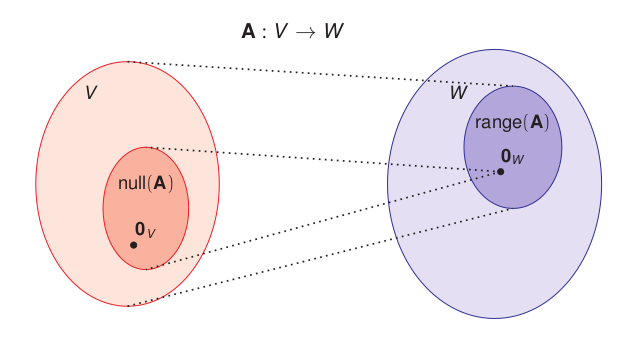
\includegraphics[width=0.5\textwidth]{null-range}
\end{figure}
\begin{definition}[Range]
  The range, or image, or $A$ is:
  \[range(A)=\left\{ w\in \mathbb{W} | \exists v\in \mathbb{V}(Av=w) \right\}.\] 
\end{definition}
We can find possible bases for the range and nullspace of a matrix using SymPy:
\begin{lstlisting}
A = np.array([[1, 2, 3],
              [4, 8, 12],
              [2, 8, 10],
              [3, 3, 6]])
mat_A = sy.Matrix(A)
print(str(sy.Matrix(A).columnspace()))
print(str(sy.Matrix(A).nullspace()))
\end{lstlisting}
\begin{definition}[Columnspace]
  The columnspace of a matrix $A\in \mathbb{R}^{n\times m}$ is the span of the $m$ columns.
  \[C(A)=range(A).\] 
\end{definition}
\begin{definition}[Rowspace]
  The rowspace of a matrix $A\in \mathbb{R}^{n\times m}$ is the span of the $n$ rows.
  \[R(A)=range(A^{T}).\] 
\end{definition}
\begin{lstlisting}
A = np.array([[1, 2, 3],
              [4, 8, -1],
              [2, 8, 2],
              [3, 3, 0]])
mat_A = sy.Matrix(A)
\end{lstlisting}
\begin{definition}[Rank]
 $rank(A)=\dim(C(A))=\dim(R(A))=\dim(range(A))$
\end{definition}
\begin{definition}[Nullity]
  $nullity(A)=\dim(null(A))$
\end{definition}
Some results for the rank of a matrix:
\begin{itemize}
  \item $rank(A)\le \min(n,m)$
  \item $rank(AB)\le rank(A)$
  \item $rank(AB)\le \min(rank(A), rank(B))$
\end{itemize}
\begin{theorem}[Rank-Nullity Theorem]
  $rank(A) + nullity(A)=m$
\end{theorem}
\begin{lstlisting}
A = np.array([[1, 2, 3],
              [4, 8, -1],
              [2, 8, 2],
              [3, 3, 0]])
print('rank A = ' + str(LA.matrix_rank(A)))
print('rank A = ' + str(LA.matrix_rank(A)))
print('nullity A = ' + str(A.shape[1] - LA.matrix_rank(A)))
\end{lstlisting}

\subsection{Geometrical Structure}
\subsubsection{Length, Similarity, Angle}
To equip a vector space with a notion of length, we equip the vector space with
a \emph{norm}.
\begin{definition}[Norm]
  A function on a real vector space $\mathbb{V}$, $\left \lVert \cdot
  \right\rVert : \mathbb{V}\mapsto \mathbb{R}$ for $\forall x,y\in
  \mathbb{V}, \forall\alpha\in \mathbb{R}$:
  \begin{itemize}
    \item $\left \lVert x \right \rVert \ge 0 $, with equality $\iff x=0$
    \item $\left \lVert \alpha x \right \rVert =\left| \alpha \right| \left \lVert x \right \rVert$
    \item $\left \lVert x+y \right \rVert\le \left \lVert x \right \rVert+\left \lVert y \right \rVert$
  \end{itemize}
\end{definition}
\begin{example}[Norms]
  We commonly define the $l_p$ norm as follows:
  \[\left \lVert x \right \rVert_p = {(\sum_{i=1}^{n} \left| x_i \right| ^{p})}^{\frac{1}{p}}.\] 
  In particular, we use the $l_1,l_2$ norms:
  \[\left \lVert x \right \rVert_1 = \sum_{i=1}^{n} \left| x_i \right|.\] 
  \[\left \lVert x\right \rVert_2 = \sqrt{\sum_{i=1}^{n} {(x_i)}^{2}}.\] 
\end{example}
\begin{lstlisting}
x_vec = np.array([x_1, x_2]).reshape(-1,1)
l1_norm = LA.norm(x_vec, 1)
l2_norm = LA.norm(x_vec, 2)
\end{lstlisting}
To equip a vector space with a notion of similarity, we equip the vector space with
a \emph{inner product}.
\begin{definition}[Norm]
  A function on a real vector space $\mathbb{V}$, $\left<\cdot,\cdot \right> :
  \mathbb{V}\times \mathbb{V}\mapsto \mathbb{R}$ for $\forall x,y,z\in
  \mathbb{V},\forall\alpha\in \mathbb{R}$:
  \begin{itemize}
    \item $\left<x,x \right> \ge 0$ with equality $\iff x=0$ 
    \item $\left<x+y,z \right> =\left<x,z \right> +\left<y,z \right>$
    \item $\left<\alpha x,y \right> =\alpha\left< x,y\right> $
    \item $\left<x,y \right> =\left<y,x \right> $
  \end{itemize}
  An inner product on $\mathbb{V}$ induces a norm on $\mathbb{V}$.
\end{definition}
\begin{example}[Dot Product]
  For Euclidean space the standard inner product is the \emph{dot product}:
  \[\left<x,y \right> =x\cdot y=\sum_{i=1}^{n} x_{i}y_{i}=x^{T}y.\]
  which induces the $l_2$ norm.
\end{example}
In addition, we define the notion of angle $\theta$ between two vectors $x,y\in
\mathbb{V}$ via the dot product:
\[x\cdot y=\left \lVert x \right \rVert_2 \left \lVert y \right \rVert_2 \cos{\theta}.\] 
\begin{lstlisting}
x_vec = np.array([x_1, x_2]).reshape(-1,1)
y_vec = np.array([y_1, y_2]).reshape(-1,1)
l2_norm_x = LA.norm(x_vec, 2)
l2_norm_y = LA.norm(y_vec, 2)
dot_product = np.dot(np.squeeze(x_vec), np.squeeze(y_vec))
cos = dot_product/(l2_norm_x * l2_norm_y)
theta_deg = 360*np.arccos(cos)/(2 * mt.pi)
\end{lstlisting}
\subsubsection{Orthonormality}
\begin{definition}[Orthonormal]
  Two vectors $x, y \in \mathbb{V}$ are said to be orthonormal if $\left \lVert
  x \right \rVert_1 =1,\left \lVert y \right \rVert_1 =1$ and they are
  orthogonal vectors (ie. $\left<x,y \right> =0$).
\end{definition}
\begin{definition}[Orthogonal Matrix]
  A square matrix $Q\in \mathbb{R}^{n\times n}$ is orthogonal if its columns
  are orthonormal:
  \[Q^{T}=Q^{-1}.\] 
\end{definition}
Multiplication by an orthogonal matrix can be considered to be a mapping that
preserves vector length while rotating or reflecting the vector about the
origin.\\
\[(Qx)\cdot(Qy)=x\cdot y.\] 
A rectangular matrix $\tilde{Q}\in \mathbb{R}^{n\times m}$ with orthonormal
columns has a transpose that is the left inverse of itself:
\[{\tilde{Q}}^{T}\tilde{Q}=I_m\text{  but  } \tilde{Q}{\tilde{Q}}^{T}\neq I_{n}.\] 
\subsubsection{Projections}
\begin{definition}[Projection]
  A projection $P_\mathbb{U}: \mathbb{V}\mapsto \mathbb{U}$ is a linear mapping
  from a vector space $\mathbb{V}$ to a subspace of $\mathbb{V}$,
  $\mathbb{U}\subseteq \mathbb{V}$ such that
  \[P_\mathbb{U}P_\mathbb{U}=P_\mathbb{U}\implies P_\mathbb{U}P_\mathbb{U}v=P_\mathbb{U}\]
\end{definition}
\begin{example}[Orthogonal Projections]
  In Euclidean space, we consider orthogonal projections which map a vector
  $x\in \mathbb{R}^{n}$ to a vector $P_\mathbb{U}x\in \mathbb{U}\subseteq
  \mathbb{R}^{n}$ such that $\left \lVert x-P_\mathbb{U}x \right \rVert_2 $ is
  minimised (it is closest to $x$). In other words, for a line $\bar{a}+t
  \bar{b}$, we seek a $P_\mathbb{U}\in \mathbb{R}^{n\times n}$ such that
  \begin{itemize}
    \item $P_\mathbb{U}x=\lambda b$ for some $\lambda\in \mathbb{R}$
    \item ${\left \lVert x-P_\mathbb{U}x \right \rVert_2} ^{2}$ is minimal
  \end{itemize}
  Hence:
  \[P_\mathbb{U}=\frac{b{b}^{T}}{{\left \lVert b \right \rVert_2} ^2}.\]
\end{example}
\begin{proof}
  We seek $\lambda$ that satisfies:
  \[\argmin_\lambda{{\left \lVert x-\lambda b \right \rVert_2}^{2} }.\] 
  Differentiating with respect to $\lambda$ for stationary points yields:
  \[2(x-\lambda b)\cdot b=0 \implies \lambda=\frac{x\cdot b}{{\left \lVert b \right \rVert_2}^{2} }.\] 
  and that $(x-P_\mathbb{U}x)$ is orthogonal to $b$.
  Furthermore, we have:
  \[P_\mathbb{U}x=\lambda b=b\lambda=b\frac{x\cdot b}{{\left \lVert b
  \right\rVert_2}^2 }=b\frac{b^{T}x}{{\left \lVert b
\right\rVert_2}^{2}}=\frac{b{b}^{T}}{{\left \lVert b \right \rVert_2 }^{2}}x.\] 
\end{proof}
\begin{example}[Generalised Orthogonal Projections]
  In general, for an $m$-dimensional subspace $\mathbb{U}\subseteq
  \mathbb{R}^{n}$ passing through the origin of basis vectors $\left\{ b_i
  \right\} _{i=1}^m$:
  \begin{itemize}
    \item $P_\mathbb{U}x=\sum_{i=1}^{m} \lambda_i b^i=B\lambda$, where $B=\left[
      b_1,\ldots,b_m \right]\in \mathbb{R}^{n\times m}$
    \item ${\left \lVert x-P_\mathbb{U}x \right \rVert_2 }^{2}$ is minimal
  \end{itemize}
  We seek $\lambda$ satisfying:
  \[\argmin_\lambda{{\left \lVert x-B\lambda \right \rVert_2 }^{2}}.\]
  Differentiating with respect to $\lambda$, $2B^{T}(x-B\lambda)=0$ implies
  $(x-P_\mathbb{U}x)$ is orthogonal to $b_i$ for all $i $, and
  \[\lambda={(B^{T}B)}^{-1}B^{T}x.\] 
  We have:
  \[P_\mathbb{U}=B{(B^{T}B)}^{-1}B^{T}.\] 
\end{example}

\subsection{Linear Equations}
One of the key uses of linear algebra is in the solution of systems of linear
equations. For known $A\in \mathbb{R}^{n\times m},b\in \mathbb{R}^{n}$ we would
like to solve for an unknown $x\in R^{m}$ where
\[Ax=b.\]
This is equivalent to a set of $n$ equations:
\begin{align*}
    A_{11} x_1 + A_{12} x_2 +\cdots  + A_{1m} x_m &= b_1 \\
    A_{21} x_1 + A_{22} x_2 +\cdots + A_{2m} x_m &= b_2 \\
    \vdots\\
    A_{n1} x_1 + A_{n2} x_2 +\cdots + A_{nm} x_m &= b_n
\end{align*}
This system of equations can have a \emph{unique solution}, \emph{no
solutions}, or \emph{infinitely many solutions}, but it cannot have more than 1
and less than an infinite number of solutions. 

\subsection{Matrix Decomposition}
\begin{definition}[Determinants]
  Determinants are defined for square matrices only. For square matrix $A$, the
  determinant is denoted $\det(A)$ or $\left| A \right|$.
\end{definition}
\begin{example}[For $A\in\mathbb{R}^{2\times2}$]
  \[\det(A)=\begin{vmatrix} A_{11}&A_{12}\\A_{21}&A_{22} \end{vmatrix}=A_{11}A_{22}-A_{21}A_{12}.\]
\end{example}
\begin{example}[For $A\in\mathbb{R}^{3\times3}$]
  \[\det(A)=\begin{vmatrix}
    A_{11}&A_{12}&A_{13}\\A_{21}&A_{22}&A_{23}\\A_{31}&A_{32}&A_{33}\end{vmatrix}
    =A_{11} \begin{vmatrix} A_{22}&A_{23}\\A_{32}&A_{33}\end{vmatrix} -A_{12}
    \begin{vmatrix} A_{21}&A_{23}\\A_{31}&A_{33} \end{vmatrix}
    +A_{13}\begin{vmatrix} A_{21}&A_{22}\\A_{31}&A_{32} \end{vmatrix}.\] 
\end{example}
\begin{example}[For $A\in\mathbb{R}^{n\times n}$]
  \[\det(A)=\sum_{j=1}^{n} {(-1)}^{i+j}A_{ij}\begin{vmatrix} M_{ij} \end{vmatrix}.\]
\end{example}
Geometrically, the determinant is the signed volume of the $n$-dimensional
paralleltope that results from the linear transform of $A$ on the unit
hypercube.
\begin{remark}
  Some properties of the determinant:
  \begin{itemize}
    \item $\det(I)=1$
    \item $\det(A^{T})=\det(A)$
    \item $\det(AB)=\det(A)\det(B)$ 
    \item $\det(A^{-1})={(\det(A))}^{-1}$ 
    \item $\det(\alpha A)=\alpha^{n}\det(A)$
  \end{itemize}
\end{remark}
\begin{definition}[Traces]
  Traces are defined for square matrices only. For square matrix $A\in
  \mathbb{R}^{n\times n}$, the trace is denoted $\tr(A):\mathbb{R}^{n\times
  n}\mapsto \mathbb{R}$ and is defined as the sum of the diagonal elements of
  $A$:
  \[\tr(A)=\sum_{i=1}^{n} A_{ii}.\] 
\end{definition}
\begin{remark}
  Some properties of the trace:
  \begin{itemize}
    \item $\tr(A+B)=\tr(A)+\tr(B)$ 
    \item $\tr(\alpha A)=\alpha\tr(A)$
    \item $\tr(I_{n})=n$ 
    \item $\tr(CD)=\tr(DC)$ for $C\in \mathbb{R}^{n\times k},D\in \mathbb{R}^{k\times n}$
  \end{itemize}
\end{remark}
\subsubsection{Matrix Decomposition}
\begin{definition}[Singular Value Decomposition]
  For any matrix $A\in \mathbb{R}^{n\times m}$,
  \[\mathbf{A}=\mathbf{U\Sigma V^{T}}\]
  where
  \begin{itemize}
    \item $\mathbf{U} = [\mathbf{u}_1, \mathbf{u}_2,\ldots,\mathbf{u}_n]$ is an $n \times n$ orthogonal matrix, and $\mathbf{u}_i \in \mathbb{R}^n$ are known as left-singular vectors;
    \item $\mathbf{V} = [\mathbf{v}_1, \mathbf{v}_2,\ldots,\mathbf{v}_m]$ is an $m \times m$ orthogonal matrix, and $\mathbf{v}_i \in \mathbb{R}^m$ are known as right-singular vectors;
    \item $\boldsymbol{\Sigma}$ is an $n \times m$ matrix with $\boldsymbol{\Sigma}_{ii} = \sigma_{i} \geq 0$, known as the singular values, and $\boldsymbol{\Sigma}_{ij} = 0, i \neq j$
  \end{itemize}
\end{definition}
To develop an intuition for the representation of SVD we consider the linear
transform of the matrix $A$:
 \[\mathbf{A} \mathbf{x} = \mathbf{U} \boldsymbol{\Sigma} \mathbf{V}^{T} \mathbf{x}.\] 

There are three elements to this mapping:
\begin{itemize}
  \item $\mathbf{x} \rightarrow \mathbf{Q}^T \mathbf{x}$
     This represents a rotation of $\mathbf{x}$ in $\mathbb{R}^{n}$
   \item $(\mathbf{V}^T \mathbf{x}) \rightarrow \boldsymbol{\Sigma} (\mathbf{V}^T \mathbf{x})$    
     This represents a shear of $(\mathbf{V}^T \mathbf{x})$ in the axis-aligned
     directions and also adds rows of zeroes (if $m>n$) or deletes rows from
     it (if $n>m$)
   \item $(\boldsymbol{\Sigma} \mathbf{V}^T \mathbf{x}) \rightarrow \mathbf{U} (\boldsymbol{\Sigma} \mathbf{Q}^T \mathbf{x})$    
     This represents a rotation of $(\boldsymbol{\Lambda} \mathbf{Q}^T \mathbf{x})$ inverse to the original rotation
\end{itemize}

\begin{definition}[Eigenvectors, Eigenvalues]
  For a square matrix, $\mathbf{A} \in \mathbb{R}^{n \times n}$, we say that $x$ is an
  eigenvector of $A$ corresponding to an eigenvalue, $\lambda$, if:
  \[Ax=\lambda x.\] 
  \begin{itemize}
    \item This implies that: $(\mathbf{A} - \lambda \mathbf{I})\mathbf{x} = \mathbf{0}$
    \item Therefore if ${(\mathbf{A} - \lambda \mathbf{I})}^{-1}$ exists, then the unique solution is $\mathbf{x} = \mathbf{0}$
    \item Therefore for non-trivial solutions we must demand that $\nexists \; {(\mathbf{A} - \lambda \mathbf{I})}^{-1}$
    \item Therefore for non-trivial solutions $\mbox{det}(\mathbf{A} - \lambda \mathbf{I})=0$ [by the Invertible Matrix Theorem]
    \item $\mbox{det}(\mathbf{A} - \lambda \mathbf{I})=0$ is known as the characteristic polynomial of $\mathbf{A}$ and
    its (possibly non-unique) roots determine the possible eigenvalues of our problem
  \end{itemize}
\end{definition}
\begin{definition}[Eigendecomposition]
  The eigendecomposition of a square matrix, $\mathbf{A} \in \mathbb{R}^{n \times
  n}$, with $n$ linearly independent eigenvectors, ${\left\{ \mathbf{p}_i \right\}}_{i=1}^n$ states that:
  \[\mathbf{A} = \mathbf{P} \boldsymbol{\Lambda} \mathbf{P}^{-1}\]
  where:
  \begin{itemize}
    \item $\mathbf{P} = [\mathbf{p}_1, \mathbf{p}_2,\ldots,\mathbf{p}_n]$;
    \item $\boldsymbol{\Lambda} = \mbox{diag}(\lambda_1, \lambda_2,\ldots,\lambda_n)$ 
    \item $\lambda_{i}$ is the eigenvalue associated with the eigenvector $\mathbf{q}_i$	
  \end{itemize}
  It follows that:
  \[\mbox{det}(\mathbf{A}) = \prod_{i=1}^n \lambda_i\]
  Note that such a decomposition does not exist for all matrices.
\end{definition}
\subsubsection{Symmetrical Matrix Decomposition}
\begin{definition}[Spectral Decomposition]
For $\mathbf{A} \in \mathbb{R}^{n \times n}$ is (real and) symmetric, then
there exists an orthonormal basis for $\mathbb{R}^n$ consisting of
eigenvectors of $\mathbf{A}$, ${\left\{ \mathbf{q}_i \vert \mathbf{q}_i \cdot
\mathbf{q}_j = \delta_{ij}, \quad \forall \; j \right\}}_{i=1}^n$, and the
associated eigenvalues are real. We call this particular eigendecomposition the
spectral decomposition.

From this it follows that the eigendecomposition of a real symmetric matrix, $\mathbf{A}$, is given by:
\[\mathbf{A} = \mathbf{Q} \boldsymbol{\Lambda} \mathbf{Q}^{T}\]

where:
\begin{itemize}
  \item $\mathbf{Q} = [\mathbf{q}_1, \mathbf{q}_2,\ldots,\mathbf{q}_n]$; $\qquad{\left\{ \mathbf{q}_i \vert \mathbf{q}_i \cdot \mathbf{q}_j = \delta_{ij},\quad \forall \; j \right\}}_{i=1}^n$
  \item $\boldsymbol{\Lambda} = \mbox{diag}(\lambda_1, \lambda_2,\ldots,\lambda_n)$
  \item $\lambda_{i}$ is the eigenvalue associated with the eigenvector $\mathbf{q}_i$
\end{itemize}
\end{definition}
To develop an intuition for the representation of the eigendecomposition we consider the
linear transform of the matrix $A$:
 \[\mathbf{A} \mathbf{x} = \mathbf{Q} \boldsymbol{\Lambda} \mathbf{Q}^{T} \mathbf{x}.\] 

There are three elements to this mapping:
\begin{itemize}
  \item $\mathbf{x} \rightarrow \mathbf{Q}^T \mathbf{x}$
     This represents a rotation of $\mathbf{x}$
   \item $(\mathbf{Q}^T \mathbf{x}) \rightarrow \boldsymbol{\Lambda} (\mathbf{Q}^T \mathbf{x})$    
     This represents a shear of $(\mathbf{Q}^T \mathbf{x})$ in axis-aligned directions
   \item $(\boldsymbol{\Lambda} \mathbf{Q}^T \mathbf{x}) \rightarrow \mathbf{Q} (\boldsymbol{\Lambda} \mathbf{Q}^T \mathbf{x})$    
     This represents a rotation of $(\boldsymbol{\Lambda} \mathbf{Q}^T \mathbf{x})$ inverse to the original rotation
\end{itemize}

\subsection{Quadratic Forms}
The quadratic form of a square matrix $\mathbf{M}\in \mathbb{R}^{n\times n}$ is defined:
\[\mathbf{x^{T}Mx}.\] 
\begin{remark}
  It is always possile to express the quadratic form of a square matrix $\mathbf{M}$ as the
  quadratic form of an associated symmetric matrix $\mathbf{A}=\frac{1}{2}(\mathbf{M+M^{T}})$:
  \[\mathbf{x^{T}Mx=x^{T}Ax}.\]
  And since quadratic forms are scalars, $\mathbf{x^{T}Mx=x^{T}M^{T}x}$
\end{remark}
\subsubsection{Definiteness}

A real symmetric matrix, $\mathbf{A}$, is said to be:
\begin{itemize}
  \item Positive Semidefinite (psd), denoted $\mathbf{A} \succeq 0 \iff
    \mathbf{x}^{T} \mathbf{A} \mathbf{x} \geq 0, \forall \mathbf{x} \; \neq
    \mathbf{0}$
  \item Positive Definite (pd), denoted $\mathbf{A} \succ 0 \iff \mathbf{x}^{T}
    \mathbf{A} \mathbf{x} > 0, \forall \mathbf{x} \; \neq \mathbf{0}$
  \item Negative Semidefinite (nsd), denoted $\mathbf{A} \preceq 0 \iff
    \mathbf{x}^{T} \mathbf{A} \mathbf{x} \leq 0, \forall \mathbf{x} \; \neq
    \mathbf{0}$
  \item Negative Definite (nd), denoted $\mathbf{A} \prec 0 \iff \mathbf{x}^{T}
    \mathbf{A} \mathbf{x} < 0, \forall \mathbf{x} \; \neq \mathbf{0}$
  \item Indefinite otherwise
\end{itemize}
\subsubsection{Geometric Intepretation of PD Quadratic Forms}
A function which occurs frequently in machine learning is:
\[f(\mathbf{x}) = \mathbf{x}^T \mathbf{A} \mathbf{x}\]
for some real, symmetric, positive definite $\mathbf{A}$. We are interested in
the form of solutions to the following equation:
\[c = \mathbf{x}^T \mathbf{A} \mathbf{x}\]
for some constant $c$. We have the solution:
\[\mathbf{x} = \sqrt{c} \mathbf{Q} \boldsymbol{\Lambda}^{-\frac{1}{2}}\mathbf{z} \qquad \mbox{s.t. } \Vert\mathbf{z}\Vert_2 =1\]
where:
\begin{itemize}
  \item $\mathbf{A} = \mathbf{Q} \boldsymbol{\Lambda} \mathbf{Q}^T$
  \item $\mathbf{Q}$ is the matrix comprised of ordered orthonormal eigenvectors of $\mathbf{A}$
  \item $\boldsymbol{\Lambda}$ is the diagonal matrix of the ordered eigenvalues of $\mathbf{A}$
  \item $\boldsymbol{\Lambda}^{-\frac{1}{2}}$ is the diagonal matrix of the ordered inverse of the square root of the eigenvalues of $\mathbf{A}$
\end{itemize}
[N.B. The eigenvalues of $\mathbf{A}$ are all positive thus
$\boldsymbol{\Lambda}^{-\frac{1}{2}}$ exists.]

The solution represents a mapping of three steps:
\begin{itemize}
  \item Plot a circle of radius $\sqrt{c}$
  \item Apply a scaling mapping, $\boldsymbol{\Lambda}^{-\frac{1}{2}}$ to the
    circle, stretching by a factor equal to the inverse square root of the
    eigenvalues of $\mathbf{A}$ in each of the axis directions to form an
    axis-aligned ellipse
  \item Apply a rotation mapping, $\mathbf{Q}$ to the axis aligned ellipse, so
    that it is rotated such that the axes now line up with the eigenvectors of
    $\mathbf{A}$ to form an eigenvector-aligned ellipse
\end{itemize}
Our solution is hence an ellipsoid for which:
\begin{itemize}
  \item The axes point in the direction of the eigenvectors of $\mathbf{A}$
  \item The radii are proportional to the inverse square root of the corresponding eigenvalues of $\mathbf{A}$
\end{itemize}
\subsection{Important Results}
\begin{theorem}[Invertible Matrix Theorem]
  For $A\in \mathbb{R}^{n\times n}$, the following statements are equivalent:
  \begin{multicols}{2}
    \begin{itemize}
      \item $A$ is invertible
      \item $rank(A)=n$ 
      \item $\det(A)\neq 0$
      \item The columns of $A$ are linearly dependent
      \item The rows of $A$ are linearly independent
      \item $\nexists x (Ax=0)$
    \end{itemize}
  \end{multicols}
\end{theorem}
Other useful results:
\begin{itemize}
  \item $\mathbf{X^{T}X}$ is symmetric
  \item $\mathbf{X^{T}X}\succeq0$
  \item $rank(\mathbf{X^{T}X})=rank(\mathbf{X})\le \min(n,m)$ 
  \item $\exists{(\mathbf{X^{T}X})}^{-1}\iff(rank(\mathbf{X^{T}X})=m)\iff\mathbf{X^{T}X}\succ 0$
  \item $rank(\mathbf{X^{T}X})=rank(\mathbf{X^{T}X}|\mathbf{X^{T}y}), \forall \mathbf{y}$
\end{itemize}

\section{Calculus}
\subsection{Derivatives}
\begin{definition}[Derivatives]
  A derivative defines a notion of continuous as follows:
  \[\frac{df}{dx} = \lim_{\delta \rightarrow 0} \frac{f(x+\delta) - f(x)}{\delta}.\] 
  It is the infinitessimal gradient at each particular point in the domain of a
  function.
\end{definition}
\begin{definition}[Curvature]
  The curvature of a function is the second-order derivative, a measure of how
  the gradient itself changes:
  \[\frac{d^2f}{dx^2} = f''(x) = \lim_{\delta \rightarrow 0} \frac{f'(x+\delta) - f'(x)}{\delta}.\] 
\end{definition}
\begin{definition}[Smoothness]
  We say that a function is $k$-smooth $\iff$ the $k$-th-order derivative of
  the function is defined. If all higher order derivatives exist, the function
  is referred to as ``smooth''.
\end{definition}

\subsubsection{Taylor Series}
For small changes $\delta$ about a point $x=\tilde{x}$, any smooth function $f$ can be approximated
as an infinite polynomial expansion as follows:
\[f(\tilde{x} + \delta) = f(\tilde{x}) + \delta f'(\tilde{x}) + \frac{\delta^2}{2} f''(\tilde{x})  + \frac{\delta^3}{3!} f^{(3)} (\tilde{x}) + \dots\]
As the order of the taylor expansion increases, we approach the underlying function.
\subsubsection{Taylor Expansion Results}
\[\frac{1}{1-x}=1+x+x^{2}+x^{3}+\cdots=\sum_{n=0}^{\infty} x^{n}, \left| x \right| <1.\] 
\[e^{x}=1+x+\frac{1}{2}x^{2}+\frac{1}{6}x^{3}+\frac{1}{24}x^{4}+\cdots=\sum_{n=0}^{\infty} \frac{1}{n\mathpunct{!}}x^{n}.\] 
\[\ln(1+x)=x-\frac{1}{2}x^{2}+\frac{1}{3}x^{3}-\frac{1}{4}x^{4}+\cdots=\sum_{n=0}^{\infty} \frac{{(-1)}^{n+1}}{n}x^{n}, \left| x \right| <1.\] 
\[\cos(x)=1-\frac{1}{2}x^{2}+\frac{1}{24}x^{24}-\frac{1}{720}x^{6}+\cdots=\sum_{n=0}^{\infty} \frac{{{(-1)}^{n}}}{(2n)\mathpunct{!}}x^{2n}.\] 
\[\sin(x)=x-\frac{1}{6}x^{3}+\frac{1}{120}x^{5}-\frac{1}{5040}x^{7}+\cdots=\sum_{n=0}^{\infty} \frac{{(-1)}^{n}}{(2n+1)\mathpunct{!}}x^{2n+1}.\] 

\subsection{Multivariate Calculus}
\subsubsection{Partial Derivatives, Gradients}
\begin{definition}[Partial Derivatives]
  For a multivariate function $f:(x_1,x_2,\ldots,x_{n})\mapsto
  f(x_1,\ldots,x_{n})$ that depends on $n$ variables, the partial derivative
  with respect to $x_i$ is defined as:
  \[\frac{\partial f}{\partial x_i} \lim_{\delta \to 0}=
  \frac{f(x_1,x_2,\ldots,x_i+\delta,\ldots,x_{n})-f(x_1,x_2,\ldots,x_i,\ldots,x_{n})}{\delta}.\] 
\end{definition}
\begin{definition}[Gradient Vectors]
  We also use a vector for the set of partial derivatives for the function, the
  gradient vector defined as: 
  \[\nabla_x f =\begin{bmatrix} \frac{\partial f}{\partial x_i}\\\vdots
  \\\frac{\partial f}{\partial x_{n}}  \end{bmatrix} \]
\end{definition}
\begin{remark}
  The gradient vector is always perpendicular to the contour, and points in the
  direction of steepest ascent.
  \begin{figure}[h!]
    \centering
    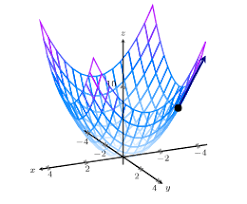
\includegraphics[width=0.3\textwidth]{gradient}
  \end{figure}\\
  In addition, we can find the slope of $f(x)$ in a particular direction $\hat{u}$ for some 
  $\left\lVert \hat{u} \right\rVert_2 =1$. This is known as the directional derivative in the direction
  of $\hat{u}$:
  \[\nabla_x f \cdot \hat{u}=\left\lVert \nabla_x f  \right\rVert_2 \left\lVert
  \hat{u} \right\rVert_2 \cos\theta.\]
  This directional derivative is maximal when $\theta=0$, when $\hat{u}$ points
  in the direction of the gradient vector (used in gradient descent).
\end{remark}

\subsubsection{Stationary Points}
\begin{definition}[Extrema]
  For a function $f:\mathbb{R}^{n}\mapsto \mathbb{R}$ and a feasible set $X\subseteq \mathbb{R}^{n}$ 
  over which we are optimising:
  \begin{itemize}
    \item A point $x$ is a local minimum of $f$ if $f(x)\le f(y) \forall y\in
      N$ where $N\subseteq X$ is some neighbourhood about $x$.
    \item A point $x$ is a global minimum of $f$ in $X$ if $f(x)\le f(y)\forall
      y\in X$
  \end{itemize}
\end{definition}
It is a necessary condition that an extrema is stationary.
\begin{definition}[Saddle Points]
  Any points for which $\nabla_x f =\mathbf{0}$ but where there is no local
  maximum or minimum are known as saddle points.
  \begin{figure}[h!]
    \centering
    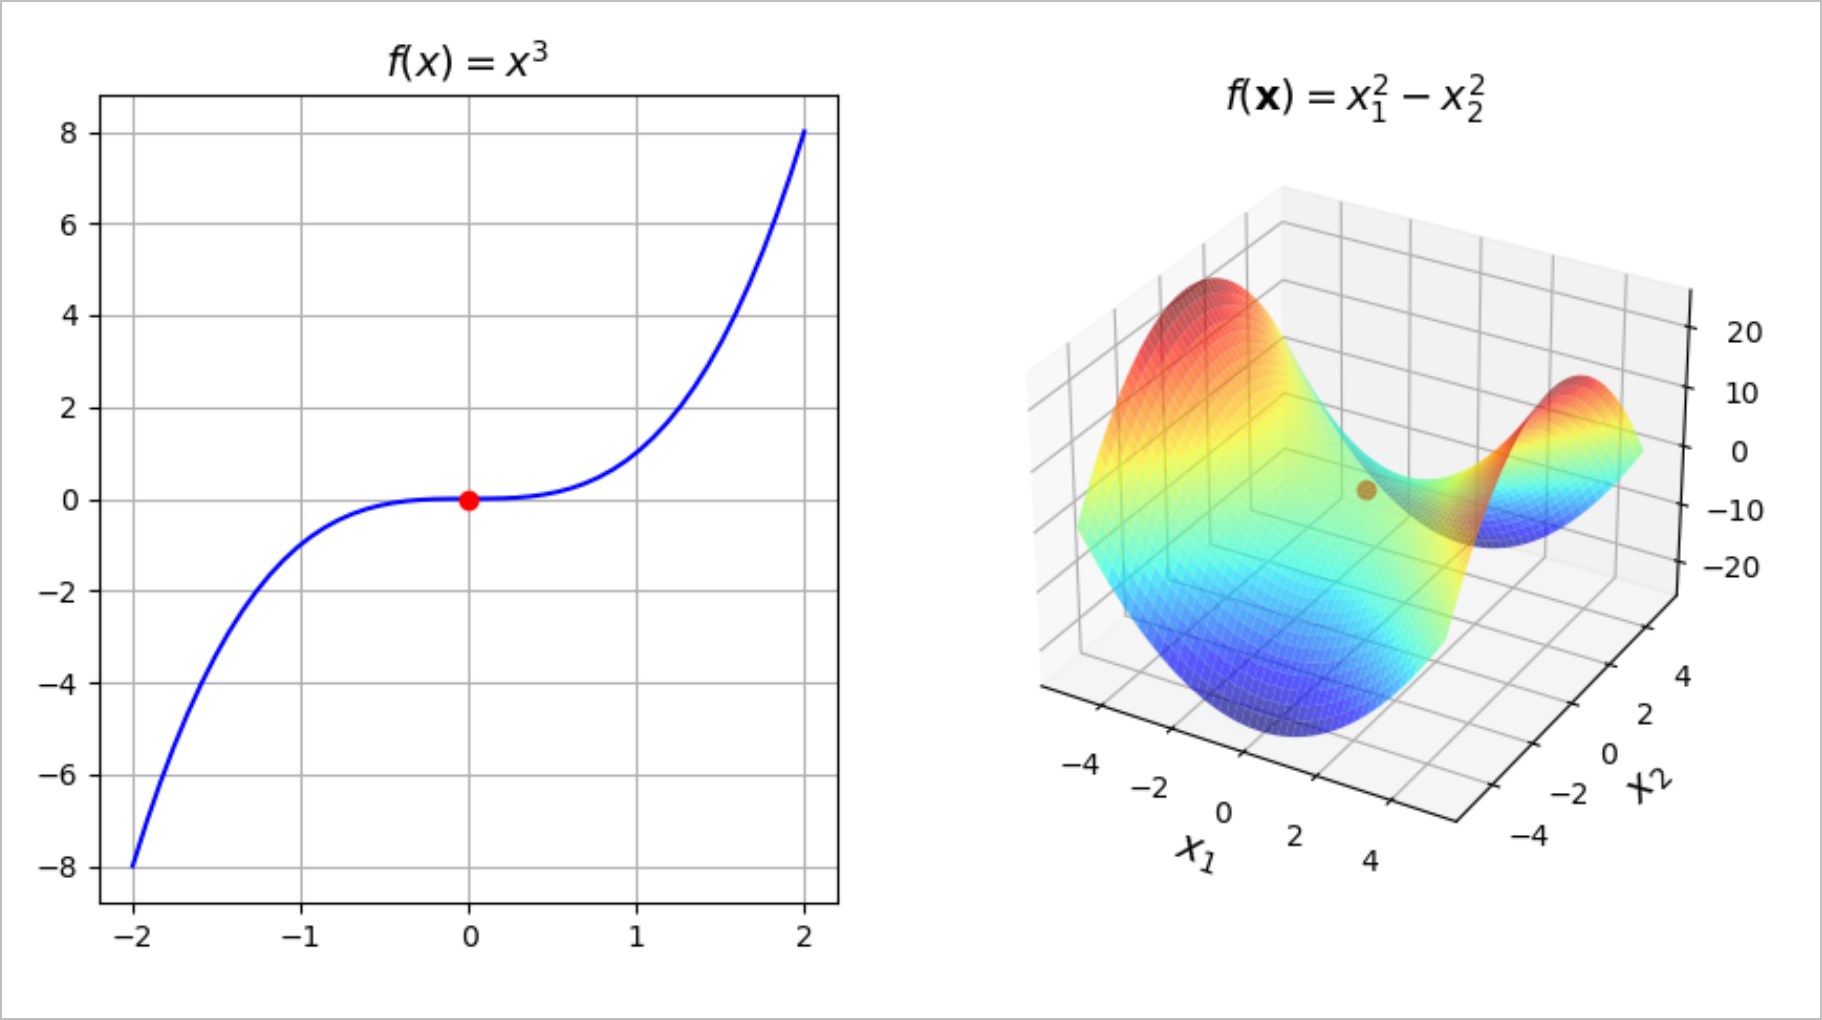
\includegraphics[width=0.8\textwidth]{saddle}
  \end{figure}
\end{definition}

\subsubsection{Hessian Matrix}
To check whether particular critical points are maxima, minima or saddle
points, we require information encoded in the second order derivatives.
\begin{definition}[Hessian Matrix]
  We define the Hessian Matrix $\nabla_x^2 f$ or $H(x)$ as:
  \[\nabla_x^2 f = \begin{bmatrix}
		\dfrac{\partial^2 f}{\partial {x_1}^2} & \cdots & \dfrac{\partial^2 f}{\partial {x_1} \partial {x_n}} \\
		\vdots & \ddots & \vdots \\
		\dfrac{\partial^2 f}{\partial {x_n} \partial {x_1}} & \cdots & \dfrac{\partial^2 f}{\partial {x_n}^2}
  \end{bmatrix}\]
\end{definition}
\subsubsection{Multivariate Taylor Series}
We can equivalently express a multivariate function using an $n$-dimensional generalisation
of the Taylor Series.
For small $\boldsymbol{\delta}$ about a point $\mathbf{x=\tilde{x}}$ in a
$2$-smooth function $f: \mathbb{F}^{n}\mapsto \mathbb{F}$:
\[f(\mathbf{\tilde{x}+\delta})\approx f(\mathbf{\tilde{x}})
\boldsymbol{\delta}^{T}\nabla_x f(\mathbf{\tilde{x}})
+\frac{1}{2}\boldsymbol{\delta}^{T}\nabla_x^2 f(\mathbf{\tilde{x}})\boldsymbol{\delta}.\] 

Thus, at a critical point, we have (for sufficiently small $\boldsymbol{\delta}$):
\[f(\mathbf{x^{*}+\delta})\approx f(\mathbf{x^{*}})
+\frac{1}{2}\boldsymbol{\delta}^{T}\nabla_x^2
f(\mathbf{{x}^{*}})\boldsymbol{\delta}.\] 
We have:
\begin{itemize}
  \item $\mathcal{H}(\mathbf{x}^*) \succ 0$ then $f(\mathbf{x}^* +
    \boldsymbol{\delta}) > f(\mathbf{x}^*)$ for all
    $\boldsymbol{\delta}\implies\mathbf{x}^*$ is a local minimum.
  \item $\mathcal{H}(\mathbf{x}^*) \prec 0$ then $f(\mathbf{x}^* +
    \boldsymbol{\delta}) < f(\mathbf{x}^*)$ for all
    $\boldsymbol{\delta}\implies\mathbf{x}^*$ is a local maximum.
  \item $\mathcal{H}(\mathbf{x}^*)$ is indefinite $\implies f(\mathbf{x}^* +
    \boldsymbol{\delta}) > f(\mathbf{x}^*)$ in certain directions, while
    $f(\mathbf{x}^* + \boldsymbol{\delta}) < f(\mathbf{x}^*)$ in other
    directions $\implies\mathbf{x}^*$ is a saddle point. 
\end{itemize}

\subsection{Convexity}
In performing optimisation, we are interested in discerning global extrema.
This is hard in general, but for twice differentiable convex functions, it is
more straightforward to do so.
\begin{definition}[Convex Set]
  A set $\boldsymbol{\Omega}$ is convex if $\forall \mathbf{x,y\in
  \Omega,\forall\theta\in} [0,1],(\mathbf{\theta
  x}+(1-\mathbf{\theta})\mathbf{y\in \Omega})$
\end{definition}
Intuitively, if we take any two elements in $\boldsymbol{\Omega}$ and draw a
line segment between the two elements, every point on that line segment belongs
to $\mathbf{\Omega}$.

\begin{definition}[Convex Function]
  A function $f: \mathbb{R}^n \to \mathbb{R}$ is convex if its domain is a
  convex set and if, $\forall\mathbf{x}_A, \mathbf{x}_B$ in its domain, and
  $\forall\lambda \in [0, 1]$, we have:
  \[f(\lambda \mathbf{x}_A + (1 - \lambda)\mathbf{x}_B) \leq \lambda
  f(\mathbf{x}_A) + (1 - \lambda)f(\mathbf{x}_B)\]
\end{definition}
\begin{definition}[Strictly Convex Function]
  A function $f: \mathbb{R}^n \to \mathbb{R}$ is strictly convex if its domain
  is a convex set and if, $\forall\mathbf{x}_A, \mathbf{x}_B$ in its domain,
  and $\forall\lambda \in (0, 1)$, we have:
  \[f(\lambda \mathbf{x}_A + (1 - \lambda)\mathbf{x}_B) < \lambda
  f(\mathbf{x}_A) + (1 - \lambda)f(\mathbf{x}_B)\]
\end{definition}
\begin{theorem}[Sum of Convex Functions]
   If $f(\cdot)$ is a convex function, $g(\cdot)$ is a convex function,
   $h(\cdot)$ is a strictly convex function and $\alpha,\beta>0$, then:
   \begin{itemize}
     \item $\alpha f(\cdot) + \beta g(\cdot)$ is a convex function.
     \item $\alpha f(\cdot) + \beta h(\cdot)$ is a strictly convex function.
   \end{itemize}
\end{theorem}
\begin{theorem}[Second Order Differential and Convexity]
  For 2-smooth $f$ over an open domain:
  \[\nabla_{\mathbf{x}}^2 f(\mathbf{x}) \succeq 0 \quad \forall \mathbf{x} \in
  \mbox{dom}(f)  \quad \iff \quad \mbox{Convexity of }f\]
  \[\nabla_{\mathbf{x}}^2 f(\mathbf{x}) \succ 0 \quad \forall \mathbf{x} \in \mbox{dom}(f)  \quad \implies \quad \mbox{Strict Convexity of }f\]
\end{theorem}
\subsubsection{Global Optimality}
Convexity is important in machine learning as it allows for the possibility to
discern global extrema for such functions. For convex and differentiable $f$,
any critical point is a globally optimal solution. Furthermore, for strictly
convex $f$ on a convex set $\boldsymbol{\Omega}$, the optimal solution is
unique.

\subsection{Quadratic Functions}
Consider the following general quadratic function:
\[f(\mathbf{x})=\mathbf{x^{T}Ax+b\cdot x}+c\]
for some $\mathbf{A}\in \mathbb{R}^{n\times n},\mathbf{b}\in
\mathbb{R}^{n},c\in \mathbb{R}$, and variable $x\in \mathbb{R}^{n}$
WLOG we can re-write this as:
\[f(\mathbf{x})=\frac{1}{2}\mathbf{x^{T}Bx+b\cdot x}+c\]
for some symmetric $\mathbf{B}=(\mathbf{A+A^{T}})$.
\begin{theorem}[Convexity of Quadratic Functions]
  The convexity of a quadratic function is entirely determined by the
  definiteness of $\mathbf{B}$.
  \begin{align*}
      \mathbf{B} \succeq 0 \quad &\iff \quad \mbox{Convexity of }f \\
      \mathbf{B} \succ 0 \quad &\iff \quad \mbox{Strict Convexity of }f
  \end{align*}
\end{theorem}
\subsubsection{Optimisation of Quadratic Functions}
Consider the unconstrained optimisation problem for some real symmetric $\mathbf{B}$:
\[f(\mathbf{x})=\frac{1}{2}\mathbf{x^{T}Bx+b\cdot x}+c, \quad \min_{\mathbf{x}}f(\mathbf{x})\]

\begin{tabular}{c c c c}
  \toprule
  Parameters of $f$& Convexity of $f$ & \# &  \\
  \midrule
  $\mathbf{B}\succ 0$ & Strictly Convex & 1 & $\mathbf{(Bx=-b)}$ consistent, exactly determined \\
  $\mathbf{B}\succeq 0,\mathbf{B}\nsucc 0,\mathbf{b}\in range(\mathbf{B})$ & Convex \& Bounded Below & $\infty$ & $(\mathbf{Bx=-b})$ consistent, underdetermined \\
  $\mathbf{B}\succeq 0,\mathbf{B}\nsucc 0, \mathbf{b}\notin range(\mathbf{B})$ & Convex \& Unbounded Below & 0 & $(\mathbf{Bx=-b})$ inconsistent \\
  $\mathbf{B}\nsucceq 0$ & Non-Convex & 0 & $f$ unbounded below \\
  \bottomrule
\end{tabular}


\section{Probability and Statistics}
\subsection{Probability Results and Concentration Inequalities}
Some probability results:
\begin{itemize}
  \item Principle of Inclusion Exclusion (PIE)
    \begin{equation*}
      \begin{split}
        P(\bigcup\limits_{i=1}^n E_i)	 =P(E_1\cup E_2\cup\ldots\cup E_n)
           & =\sum\limits_{i=1}^{n}P(E_i)-\sum\limits_{i_1<i_2}P(E_{i_1}E_{i_2})+\ldots\\
                                      & +{(-1)}^{r+1}\sum\limits_{i_1<i_2<\cdots<i_r}P(E_{i_1}E_{i_2}\ldots E{i_r})
           +\cdots+{(-1)}^{n+1}P(E_1E_2\ldots E_n)
      \end{split}
    \end{equation*}
  \item $\begin{aligned}[t]
      P(\bigcup\limits_{i=1}^n E_i)\le&\sum\limits_{i=1}^{n}P(E_i)\\
      \ge&\sum\limits_{i=1}^{n}P(E_i)-\sum\limits_{j<i}P(E_{i}E_j)\\
      \le&\sum\limits_{i=1}^{n}P(E_i)-\sum\limits_{j<i}P(E_{i}E_j)+\sum\limits_{k<j<i}P(E_{i}E_{j}E_{k})
    \end{aligned}$
  \item \( P(E_{1}E_{2}…E_{n}) = P(E_{1}) P(E_{2}|E_{1})…P(E_n|E_{1}…E_{n-1})\)
  \item For $F_1,F_2,…,F_n$ partitioning $S$,
    \[ P(E) = \sum_{i=1}^{n} P(EF_i) = \sum_{i=1}^{n} P(F_i) P(E|F_i) \] 
  \item Baye's Theorem: $E$ occurred. Which $F_j$ most likely led to $E$:
    \begin{equation*}
      \begin{split}
        P(F_j|E) & = \frac{P(EF_j)}{P(E)} = \frac{P(F_j)P(E|F_j)}{P(E)}\\
                 & = \frac{P(F_j)P(E|F_j)}{\sum_{i=1}^{n} P(F_i)P(E|F_i)}
      \end{split}
    \end{equation*}
    $P(A)$ is known as the prior.\\
    $P(A|B)$ is known as the posterior.\\
    $P(B|A)$ is known as the likelihood.\\
    $P(B)$ is known as the evidence.
  \item Odds of $E=\frac{P(F)}{P(F^C)}$
\end{itemize}
Some concentration inequalities:
\begin{itemize}
  \item Markov's Inequality [For non-negative $\mathcal{X}$ with expectation $E(X)$], $\forall a>0$
    \[P(X\ge0)=1\Rightarrow P(X\ge a)\le \frac{E(X)}{a}\]
  \item Chebyshev's Inequality [For finite $\mu,Var(X)$], $\forall k>0$
  \[P(|X-\mu|>k)\le \frac{\sigma^{2}}{k^{2}}\]
  \item Hoeffding's Inequality [For i.i.d random variables $X_1,X_2,\ldots$,
    such that each is bounded $[a_i,b_i]$, and let
    $\bar{\mathcal{X}}_{n}=\frac{1}{n}\sum_{i=1}^{n} \mathcal{X}_i$],
    $\forall\epsilon>0$,
    \[P(|\bar{\mathcal{X}}-E(\bar{\mathcal{X}})|\ge\epsilon)\le2
\exp(-\frac{2n^{2}\epsilon^{2}}{\sum_{i=1}^{n} {(b_i-a_i)}^{2}})\]
  \[ P(\bar{\mathcal{X}}-E(\bar{\mathcal{X}})\ge\epsilon)\le
  \exp(-\frac{2n^{2}\epsilon^{2}}{\sum_{i=1}^{n} {(b_i-a_i)}^{2}})\]
  \item For i.i.d random variables $X_1,X_2,\ldots$, $\forall\epsilon>0$,
    \[P(|\frac{X_1+\cdots+X_n}{n}-\mu|\ge\epsilon)\to0\text{ as }n\to\infty\]
  \item For i.i.d $X_1,X_2,\ldots$ where $E(X_i)=\mu, Var(X_i)=\sigma^{2}$,
    \[\frac{X_1+\cdots+X_n-n\mu}{\sigma\sqrt{n}}\sim N(0,1)\text{ as }n\to\infty\]
\end{itemize}

\subsection{Univariate Probability Distributions}
\subsubsection{Bernoulli Distribution}
${\mathcal{X}}$ is a discrete random variable, with outcomes, $x$, which can take one of two values: 0 or 1, with a probability that $x=1$ being equal to $\theta$
\[x \sim \text{Bern}(\theta)\]
\[p_{\mathcal{X}}(x ; \theta) = \theta^x {(1-\theta)}^{1-x}\]
\[\mathbb{E}_{\mathcal{D}}[\mathcal{X}] = \theta\]
\[\text{Var}_{\mathcal{D}}[\mathcal{X}] = \theta (1-\theta)\]
\subsubsection{Binomial Distribution}
${\mathcal{X}}$ is a discrete random variable, with outcomes, $x$, that denotes
the number of successes, $k$, that we will achieve in $n$ independent Bernoulli
trials. ${\mathcal{X}}$ can be written as the sum of $n$ independent Bernoulli trials
${\left\{\mathcal{X}_i\right\}}_{i=1}^n$, with outcomes ${\{x_i \sim \mbox{Bern}(\theta)\}}_{i=1}^n$:
\[\mathcal{X} = \mathcal{X}_1 + \mathcal{X}_2 +\cdots + \mathcal{X}_n\]
This characterises the associated $\mathcal{D}$ as a Binomial Distribution:
\[x \sim \text{Bin}(n, \theta)\]
\[p_{\mathcal{X}}(k ; n, \theta) = \binom{n}{k} \theta^k {(1-\theta)}^{n-k}\]
\[\mathbb{E}_{\mathcal{D}}[\mathcal{X}] = n \theta\]
\[\text{Var}_{\mathcal{D}}[\mathcal{X}] = n \theta (1-\theta)\]
\subsubsection{Beta Distribution}
$\mathcal{X}$ be a continuous random variable, taking values $x \in [0,1]$,
such that $\mathcal{D}$ follows a Beta distribution:
\[x \sim \mbox{Beta}(a,b) \qquad \mbox{where:} \qquad a,b >0\]
This has a characteristic pdf $f_{\mathcal{X}}$:
\[f_{\mathcal{X}}(x; a, b) = \frac{\Gamma(a+b)}{\Gamma(a) \Gamma(b)} x^{a-1} {(1-x)}^{b-1} \quad \mbox{where:} \quad \Gamma(a) = \int_{0}^{\infty} u^{a-1} e^{-u} du\]
\[\mathbb{E}_{\mathcal{D}}[\mathcal{X}] = \frac{a}{a+b}\]
\[\mbox{Var}_{\mathcal{D}}[\mathcal{X}] = \frac{ab}{{(a+b)}^2(a+b+1)}\]
\subsubsection{Gaussian Distribution}
$\mathcal{X}$ is a continuous random variable, taking values $x \in
\mathbb{R}$, such that $\mathcal{D}$ follows a Gaussian distribution:
\[x \sim \mathcal{N}(\mu,\sigma^2) \qquad \text{where:} \qquad \mu \in \mathbb{R}, \sigma \in (0, \infty)\]
This has a characteristic pdf $f_{\mathcal{X}}$:
\[f_{\mathcal{X}}(x ; \mu, \sigma) = \frac{1}{\sqrt{2 \pi \sigma^2}} \exp \left( -\frac{{(x-\mu)}^2}{2 {\sigma}^2} \right)\]
\[\mathbb{E}_{\mathcal{D}}[\mathcal{X}] = \mu\]
\[\text{Var}_{\mathcal{D}}[\mathcal{X}] = \sigma^2\]


\subsection{Multivariate Probability Distribution}
\subsubsection{Covariance}
\begin{definition}[Covariance]
The covariance is a measure of the linear relationship between two random
variables, defined as:
\[\mbox{Cov}[\mathcal{X}_1, \mathcal{X}_2] = \mathbb{E}_{\mathcal{D}}\left[
(\mathcal{X}_1 - \mathbb{E}_{\mathcal{D}_1}[\mathcal{X}_1]) (\mathcal{X}_2 -
\mathbb{E}_{\mathcal{D}_2}[\mathcal{X}_2]) \right]\]
\[\mbox{Cov}[\mathcal{X}_1, \mathcal{X}_2] =
\mathbb{E}_{\mathcal{D}}\left[\mathcal{X}_1 \mathcal{X}_2 \right] -
\mathbb{E}_{\mathcal{D}_1}\left[\mathcal{X}_1 \right]
\mathbb{E}_{\mathcal{D}_2}\left[\mathcal{X}_2 \right]\]
\end{definition}
The covariance of some random vector, $\boldsymbol{\mathcal{X}} =
{[\mathcal{X}_1, \mathcal{X}_2,\ldots,\mathcal{X}_m]}^T$, with outcomes,
$\mathbf{x} \sim \mathcal{D}$, where $\mathbf{x} = {[x_1, x_2,\ldots, x_m]}^T$ and
${\{ x_i \sim \mathcal{D}_i \}}_{i=1}^m$ is characterised by the covariance
matrix:
\begin{align*}
\boldsymbol{\Sigma} &= \mathbb{E}_{\mathcal{D}} \left[ (\boldsymbol{\mathcal{X}} - \mathbb{E}_{\mathcal{D}}[\boldsymbol{\mathcal{X}}]){(\boldsymbol{\mathcal{X}} - \mathbb{E}_{\mathcal{D}}[\boldsymbol{\mathcal{X}}])}^T \right] \\
    &=\begin{bmatrix}
    \mbox{Var}[\mathcal{X}_{1}] & \mbox{Cov}[\mathcal{X}_{1},\mathcal{X}_{2}] & \cdots & \mbox{Cov}[\mathcal{X}_{1},\mathcal{X}_{m}]\\
    \mbox{Cov}[\mathcal{X}_{2},\mathcal{X}_{1}] & \mbox{Var}[\mathcal{X}_{2}] & \cdots & \mbox{Cov}[\mathcal{X}_{2},\mathcal{X}_{m}]\\
    \vdots & \vdots & \ddots & \vdots \\
    \mbox{Cov}[\mathcal{X}_{m},\mathcal{X}_{1}] & \mbox{Cov}[\mathcal{X}_{m},\mathcal{X}_{2}] & \cdots & \mbox{Var}[\mathcal{X}_{m}]\\
    \end{bmatrix}
\end{align*}
\begin{remark}
 $\boldsymbol{\Sigma}$ is symmetric and positive semidefinite.
\end{remark}
\begin{definition}[Correlation]
The correlation is the normalised covariance and always lies between -1 and 1:
\[\rho(\mathcal{X}_1, \mathcal{X}_2) = \frac{\mbox{Cov}[\mathcal{X}_1, \mathcal{X}_2]}{\sqrt{\mbox{Var}_{\mathcal{D}_1}[\mathcal{X}_1] \mbox{Var}_{\mathcal{D}_2}[\mathcal{X}_2]}}\]
We define a correlation matrix, a normalised version of the covariance matrix,
to encode a set of correlations between $m$ different random variables:
\begin{equation*}
    \boldsymbol{\rho} =\begin{bmatrix}
    1 & \frac{\mbox{Cov}[\mathcal{X}_1, \mathcal{X}_2]}{\sqrt{\mbox{Var}_{\mathcal{D}_1}[\mathcal{X}_1] \mbox{Var}_{\mathcal{D}_2}[\mathcal{X}_2]}} & \cdots & \frac{\mbox{Cov}[\mathcal{X}_1, \mathcal{X}_m]}{\sqrt{\mbox{Var}_{\mathcal{D}_1}[\mathcal{X}_1] \mbox{Var}_{\mathcal{D}_m}[\mathcal{X}_m]}}\\
    \frac{\mbox{Cov}[\mathcal{X}_2, \mathcal{X}_1]}{\sqrt{\mbox{Var}_{\mathcal{D}_2}[\mathcal{X}_2] \mbox{Var}_{\mathcal{D}_1}[\mathcal{X}_1]}} & 1 & \cdots & \frac{\mbox{Cov}[\mathcal{X}_2, \mathcal{X}_m]}{\sqrt{\mbox{Var}_{\mathcal{D}_2}[\mathcal{X}_2] \mbox{Var}_{\mathcal{D}_m}[\mathcal{X}_m]}}\\
    \vdots & \vdots & \ddots & \vdots \\
    \frac{\mbox{Cov}[\mathcal{X}_m, \mathcal{X}_1]}{\sqrt{\mbox{Var}_{\mathcal{D}_m}[\mathcal{X}_m] \mbox{Var}_{\mathcal{D}_1}[\mathcal{X}_1]}} & \frac{\mbox{Cov}[\mathcal{X}_m, \mathcal{X}_2]}{\sqrt{\mbox{Var}_{\mathcal{D}_m}[\mathcal{X}_m] \mbox{Var}_{\mathcal{D}_2}[\mathcal{X}_2]}} & \cdots & 1\\
    \end{bmatrix}
\end{equation*}
\end{definition}
\subsubsection{Multivariate Gaussian Distribution}
A random vector $\boldsymbol{\mathcal{X}} =
{[\mathcal{X}_1,\ldots,\mathcal{X}_n]}^T$, with outcomes $\mathbf{x}$, has a
multivariate Gaussian distribution if it has the following characterisation:
\[\mathbf{x} \sim \mathcal{N}(\boldsymbol{\mu},\boldsymbol{\Sigma}) \qquad \text{where:} \qquad \boldsymbol{\mu} \in \mathbb{R}^n\]
The multivariate Gaussian has the characteristic pdf
$f_{\boldsymbol{\mathcal{X}}}$:
\[f_{\boldsymbol{\mathcal{X}}}(\mathbf{x} ; \boldsymbol{\mu},\boldsymbol{\Sigma}) = \frac{1}{{(2 \pi)}^{n/2}} \frac{1}{\vert \boldsymbol{\Sigma} \vert^{1/2}} \exp \left( -\frac{1}{2}{(\mathbf{x}-\boldsymbol{\mu})}^T \boldsymbol{\Sigma}^{-1} (\mathbf{x}-\boldsymbol{\mu}) \right)\]
\[\mathbb{E}_{\mathcal{D}}[\boldsymbol{\mathcal{X}}] = \boldsymbol{\mu}\]
\[\text{Cov}_{\mathcal{D}}[\boldsymbol{\mathcal{X}}] = \boldsymbol{\Sigma}\]
The isocontours of a multivariate Gaussian are characterised by the exponent of the pdf:
\[{(\mathbf{x}-\boldsymbol{\mu})}^T {\boldsymbol{\Sigma}}^{-1} (\mathbf{x}-\boldsymbol{\mu})\]
which are ellipsoids:
\begin{itemize}
  \item centred at $\boldsymbol{\mu}$
  \item with axes pointing in the direction of the eignevectors of $\boldsymbol{\Sigma}^{-1}$
  \item having radii proportional to the square root of the corresponding eigenvalues of $\boldsymbol{\Sigma}$
\end{itemize}

\subsection{Maximum Likelihood Estimation}
\subsubsection{Likelihood}
Suppose some random variable $\mathcal{X}$ the distribution of which
$\mathcal{D}$ is parameterised by unknown variables  $\mathbf{\theta}\in
\mathbb{R}^{k}$. Suppose we make a sequence of observations of outcomes
$\mathcal{S}$ (itself an outcome of a random variable), and each $i$-th member
$x_i$, is the outcome of the random variable $\mathcal{X}$.
\begin{definition}[Likelihood Function]
  We define the likelihood function to be the joint probability function of a
  set of outcomes:
\[\mathbf{L}(\boldsymbol{\theta})=p_{\mathcal{x}_1,\ldots,\mathcal{x}_{n}}(x_1,\ldots,x_{n};\boldsymbol{\theta}).\] 
  This joint density is considered to be a function of $\boldsymbol{\theta}$.
\end{definition}
\begin{remark}
  The characterisation of the parameters $\mathbf{\theta}$ being fixed but
  unknown is definitive of the \textbf{frequentist paradigm}.
\end{remark}
\subsubsection{Likelihood of i.i.d Random Variables}
If the sequence of $\boldsymbol{\mathcal{X}}$ is i.i.d, we denote
$\mathcal{S}\sim\mathcal{D}^{n}$, and the likelihood is expressed as:
\[\mathbf{L}(\boldsymbol{\theta})=\prod_{i=1}^{n} p_{\mathcal{x}_i}(x_i;\boldsymbol{\theta}).\] 
It is easier to optimise the logarithm of the likelihood function, and we
define the log-likelihood:
\[\boldsymbol{\mathcal{L}}(\boldsymbol{\theta})=\sum_{i=1}^{n} \log\left(p_{\mathcal{X}_i}\left(x_i;\boldsymbol{\theta}\right)\right).\] 
\begin{definition}[Maximum Likelihood Estimate]
  The MLE $\boldsymbol{\theta_{MLE}}$ is the value of $\boldsymbol{\theta}$
  that maximises the likelihood function, i.e., the observed data is most
  probable with this parameterisation.
\end{definition}
\begin{notation}[$\boldsymbol{\theta}^{*}$]
  We define $\boldsymbol{\theta}^{*}$ to be the true unknown value of
  $\boldsymbol{\theta}$.
\end{notation}

\subsection{Maximum A Posteriori Estimation}
The Maximum A Posteriori estimator is defined:
\[\theta_{MAP}=\argmax_\theta \left\{ p_\Theta\left( \theta|S \right)  \right\}.\] 
As $n$ becomes large (as we gather more data), the prior distribution becomes less influential and
the posterior becomes dominated by the likelihood function.\ i.e.\ as $n \to\infty$:
\[\theta_{MAP}\to\theta_{MLE}\quad\text{and}\quad\mu_{MAP}\to\mu_{MLE}.\] 

\section{Regression}
\subsection{Linear Regression}
In Linear Regression we learn a mapping $\mathbf{f_w}:\mathbb{R}^{m}\mapsto
\mathbb{R}$ between input attributes $x$ and a single output $y$,
drawn from a function class $\mathcal{F}$:
\[\mathcal{F}=\left\{ \mathbf{f_w(X)=w\cdot x|w}={\left[ w_0,w_1,\ldots,w_m \right]}^{T}\in \mathbb{R}^{m+1} \right\}.\] 
$\mathbf{f_w}$ is characterised by a weight vector $\mathbf{w}$ of which we define:
\[\mathbf{f_w(x)=w\cdot x,\quad x}={[1,x_1,\ldots,x_m]}^{T}\]
\subsubsection{Training Data}
Suppose we draw $n$ observations, each consisting $m$ features (each $i$-th
observation encoded $x^{(i)}\in \mathbb{R}^{m}$), as well as the output labels
$y_i\in \mathbb{R}$. We represent our output training data as $y$:
\[\mathbf{y}=\begin{bmatrix} y^{(1)}\\y^{(2)}\\\vdots\\y^{(n)} \end{bmatrix}.\] 
\begin{definition}[Design Matrix]
  To represent the input attribute data more compactly, we define the design matrix $X$:
  \[\mathbf{X}=\begin{bmatrix}
    \mathbf{x}^{(1)T}\\\mathbf{x}^{(2)T}\\\vdots\\\mathbf{x}^{(n)T}
    \end{bmatrix} =\begin{bmatrix}
  1&x_1^{(1)}&\cdots&x_m^{(1)}\\
  1&x_2^{(2)}&\cdots&x_m^{(2)}\\
  \vdots&\vdots&\ddots&\vdots\\
  1&x_1^{(n)}&\cdots&x_m^{(n)}
\end{bmatrix}.\] 
\end{definition}
We therefore seek $\mathbf{w}$ such that $\mathbf{y=Xw}$. We have a solution
only if $rank(\mathbf{X})=rank(\mathbf{X|y})=(m+1)\le n$. In general this is
not true.

\subsubsection{Evaluation}
To make the problem well-defined, we choose an evaluation function
to help us select the optimal weight vector. We consider the empirical squared
error evaluation function:
\[L(\mathcal{E},\mathcal{S},\mathbf{f_w})=\frac{1}{2n}\sum_{i=1}^{n} {(y^{(i)}-\mathbf{w\cdot x^{(i)}})}^{2}.\] 
We seek the $\mathbf{w}$ at which this evaluation function is minimised.
\[\mathbf{w}_{OLS}=\argmin_\mathbf{w}\left(\frac{1}{2}\sum_{i=1}^{n} {(y^{(i)}-\mathbf{w\cdot x^{(i)}})}^{2}\right).\] 
The optimal ${\mathbf{w}}_{OLS}$ is known as the Ordinary Least Squares
estimator and this approach is known as OLS regression.
Assuming the features and the output are related by an additive noise model:
\[y^{(i)}=\mathbf{w\cdot x}^{(i)}+\epsilon^{(i)}.\]
The Gauss Markov Theorem demonstrates that $\mathbf{w}_{OLS}$ is the Best
Linear Unbiased Estimator (BLUE).
Further assuming the noise is normally distributed:
\[\epsilon\sim\mathcal{N}(0,\sigma^{2})\quad \implies\quad
\mathbf{y|x}\sim\mathcal{N}(\mathbf{w\cdot x}, \sigma^{2})\] 
The Maximum Likelihood Estimator $\mathbf{w}_{MLE}$ is:
\begin{align*}
  \mathbf{w}_{MLE}=&\argmax_\mathbf{w}{\left\{\ln\left( \prod_{i=1}^{n} \frac{1}{\sqrt{2\pi\sigma^{2}}}\exp\left(-\frac{{(y^{(i)}-w\cdot x^{(i)})}^{2}}{2\sigma^{2}}\right)  \right)\right\} }\\
  =&\argmax_\mathbf{w}{\sum_{i=1}^{n} \ln\left( \frac{1}{\sqrt{2\pi\sigma^{2}}}\exp\left(-\frac{{(y^{(i)}-w\cdot x^{(i)})}^{2}}{2\sigma^{2}}\right)  \right) }\\
  =&\argmax_\mathbf{w}{\left(-n \ln \sqrt{2\pi\sigma^{2}} - \sum_{i=1}^{n} \left(\frac{{(y^{(i)}-w\cdot x^{(i)})}^{2}}{2\sigma^{2}}\right)  \right) }\\
  =&\argmin_\mathbf{w}{\left( \frac{1}{2}\sum_{i=1}^{n} {\left(y^{(i)}-\mathbf{w\cdot x}^{(i)}\right)}^{2} \right) }\\
  =&\mathbf{w}_{OLS}
\end{align*}

\subsection{Linear Regression --- Analytic Solution}
\subsubsection{Critical Points}
We first find the gradient of the loss function:
\begin{align*}
  L(\mathcal{E},\mathcal{S},f_w)=&\frac{1}{2n}{\left\lVert \mathbf{y-Xw} \right\rVert_2}^2\\
  =&\frac{1}{2n}\mathbf{{(y-Xw)}^{T}(y-Xw)}\\
  \nabla_w L =& \frac{1}{2n}\nabla_w \left(\mathbf{{(y-Xw)}^{T}(y-Xw)}\right)\\
  =& \frac{1}{2n}\nabla_w\left( \mathbf{y^{T}y-y^{T}Xw-w^{T}X^{T}y+w^{T}X^{T}Xw}\right)\\
  =&\frac{1}{2n}\nabla_w\left(\mathbf{w^{T}X^{T}Xw-2y^{T}Xw}\right) \\
  =&\frac{1}{n} \left( \mathbf{X^{T}Xw-X^{T}y} \right)
\end{align*}
and solve for the criticial points of the function:
\begin{align*}
  \nabla_w L =& 0\\
  0=&\frac{1}{n} \left( \mathbf{X^{T}Xw}_{OLS}-\mathbf{X^{T}y} \right)\\
  \mathbf{X^{T}Xw}_{OLS}=&\mathbf{X^{T}y}
\end{align*}
Since $rank(\mathbf{X^{T}X})=rank(\mathbf{X^{T}X|X^{T}y})$, the system is
consistent and we have one or infinitely many solutions.\\
If ${(\mathbf{X^{T}X})}^{-1}$ exists we have the unique solution:
\[\mathbf{w}_{OLS}=\mathbf{(X^{T}X)}^{-1}\mathbf{X^{T}y}.\]
known as the \textbf{Normal Equations} with an analytic solution to the OLS approach.\\
\begin{itemize}
  \item \textbf{Representation} \[\mathcal{F}=\left\{ \mathbf{w\cdot x}|\mathbf{w}\in \mathbb{R}^{m+1} \right\}\]
  \item \textbf{Evaluation} \[\frac{1}{2}\sum_{i=1}^{n} {(y^{(i)}-\mathbf{w\cdot x^{(i)}})}^{2}\]
  \item \textbf{Optimisation} \[\mathbf{w}_{OLS}=\argmin_\mathbf{w}\left\{
      \frac{1}{2}\sum_{i=1}^{n} {(y^{(i)}-\mathbf{w\cdot x^{(i)}})}^{2} \right\}\]
\end{itemize}
If ${(\mathbf{X^{T}X})}$ is non-invertible then $rank(\mathbf{X^{T}X})<(m+1)$,
the problem is undetermined and we have an infinite number of solutions. This
is known as overfitting.
\begin{figure}[h!]
  \centering
  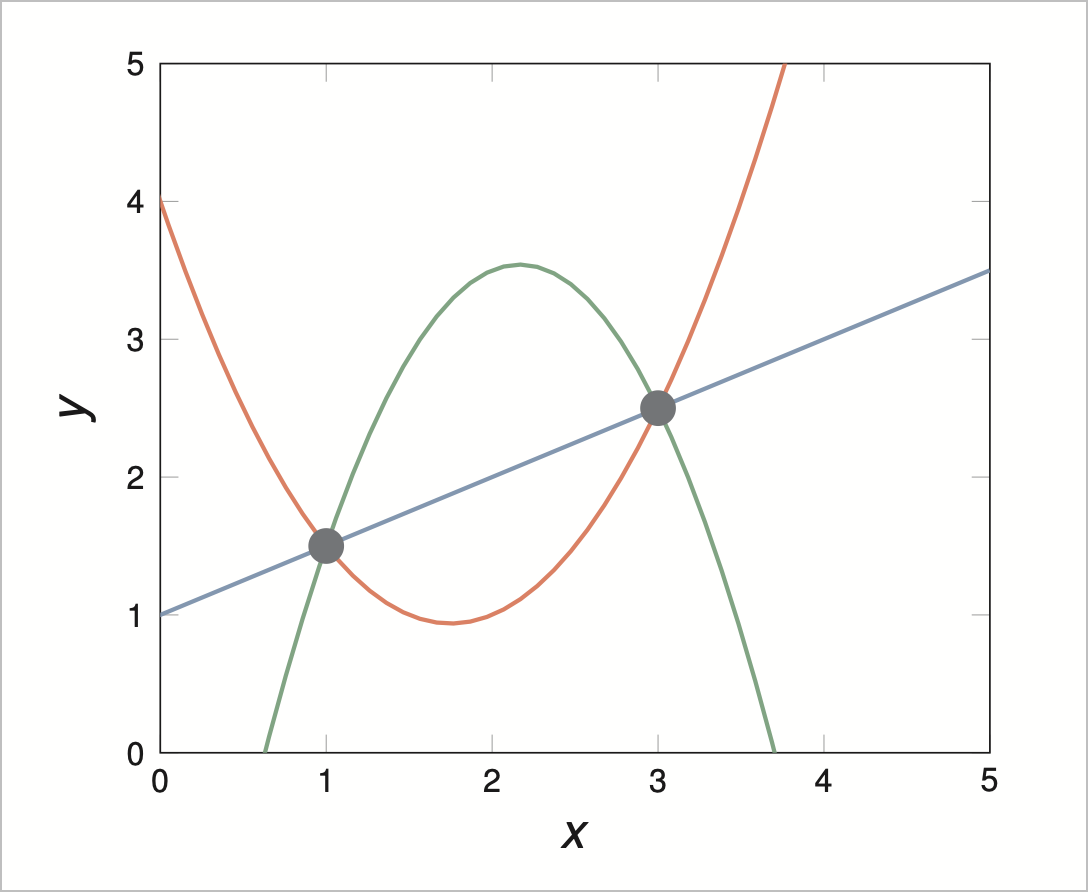
\includegraphics[width=0.4\textwidth]{overfitting}
\end{figure}
\subsubsection{Optimality}
To check for the optimality of the solution, we first obtain the Hessian:
\[\nabla_w^{2}L=\mathbf{X^{T}X}\]
Since the Hessian matrix is positive semidefinite
($\mathbf{a^{T}X^{T}Xa={\left\lVert Xa \right\rVert_2}^{2}}\ge 0\quad \forall
\mathbf{a}\in \mathbb{R}^{m+1}$), L is convex and a critical point is globally
optimal
\subsubsection{Uniqueness}
Uniqueness of the solution requires that Hessian is positive definite
$\iff\mathbf{(X^{T}X)}^{-1}$, such that the function is strictly convex.
Otherwise, the function is not strictly convex (but still bounded since
$\mathbf{X^{T}y}\in range(\mathbf{X^{T}X})$).
\begin{remark}
  Matrix Derivation Results w.r.t. $w$:
  \begin{itemize}
    \item Linear form: \(a^T w\implies\nabla_w (a^T w) = a\) for some constant vector \(a\)
    \item Quadratic form: \(w^T A w \implies\nabla_w (w^T A w) = (A + A^T) w\)for some constant matrix \(A\)
  \end{itemize}
\end{remark}
\subsubsection{Limitations}
The problem does not scale well with the dimensionality of the input attributes
$m$. Matrix inversion requires $O(m^{3})$ operations --- which is expensive for
large $\mathbf{X^{T}X}$. There are also space constraints for very high $m$ to
store $\mathbf{X^{T}X}$.

\subsection{Linear Regression --- Numerical Optimisation}
To overcome these limitations, we consider a first order iterative numerical
optimisation algorithm, \textbf{Gradient Descent}. Intuitively, we take steps proportional
to the negative of the gradient (which is in the direction of steepest descent)
at each step.
\subsubsection{Batch Gradient Descent}
\begin{lstlisting}
def LinearRegression_OLS_GD(X, y, w_init, alpha, max_epoch=10):
    n = len(y)
    w_t = w_init
    L_hist = (1/(2*n)) * (y + np.matmul(X, w_t)).T.dot(y - np.matmul(X, w_t))
    w_hist = w_t.T
    epoch = 0
    while epoch < max_epoch:
        grad = (1/n) * X.T.dot(X.dot(w_t) - y).reshape(np.shape(X)[1], 1)
        w_t = (w_t - alpha * grad)
        loss = (1/(2*n)) * (y - X.dot(w_t)).T.dot(y - X.dot(w_t))[0][0]
        L_hist = np.vstack((L_hist, loss))
        w_hist = np.vstack((w_hist, w_t.T))
        epoch += 1
    return w_hist, L_hist
\end{lstlisting}
$\alpha>0$ is the learning rate which determines the step size (factor of
proportionality to the gradient).For $\alpha$ too small, convergence is slow,
and for $\alpha$ too large, we get divergence.\\
Since the loss function is a convex objective, gradient descent guarantees the
local optimum found is a global optimum. However, Batch Gradient Descent may be
costly, as we need to scan through the entire training set for each step.
\begin{figure}[h!]
  \centering
  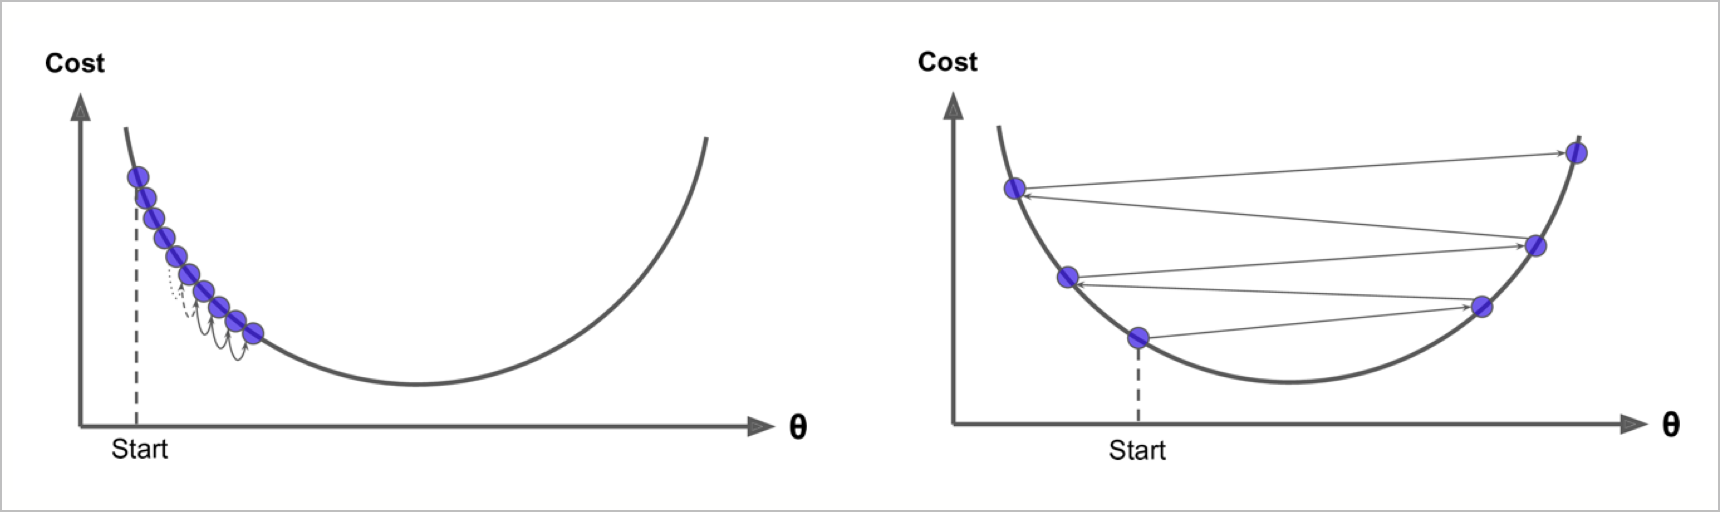
\includegraphics[width=0.7\textwidth]{learning-rate}
\end{figure}
\subsubsection{Stochastic Gradient Descent}
\begin{figure}[h!]
  \centering
  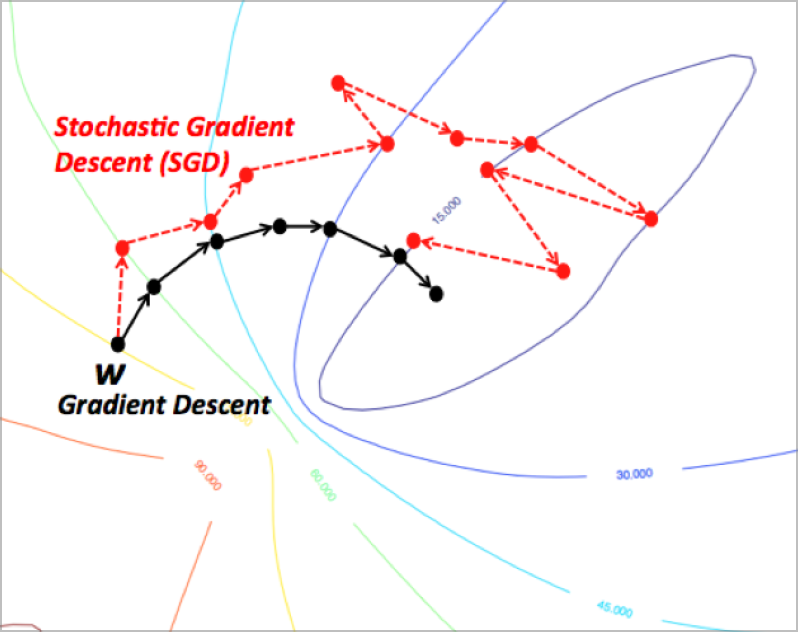
\includegraphics[width=0.4\textwidth]{sgd}
\end{figure}
In Stochastic Gradient Descent, we randomly shuffle the dataset for each step,
and estimate the gradient using one observation. Hence, each SGD update is less
optimal than a BGD update, and it will not converge monotonically, but overall
convergence is generally faster.
\subsubsection{Data Scaling}
For multi-dimensional data, even if we make an optimal setting of the learning
rate, \textbf{ill-conditioning} of the loss surface may result in a slow
convergence. This is caused by the gradient of the largest attribute dominating
the overall gradient. We may alleviate the effect through data scaling to scale our attributes. This
ensures that all parameters are updated in similar proportions, leading to
faster convergence.

\subsection{Polynomial Regression}
In Polynomial Regression we learn a mapping $\mathbf{f_W}:\mathbb{R}^{m}\mapsto
\mathbb{R}$ between input attributes $x$ and an output $y$ drawn from a function
class $\mathcal{F}$.$\mathbf{f_w}$ is characterised by a weight vector $\mathbf{w}$:
\[\mathbf{f_w}=w\cdot \hat{z}\]
for some vector $\hat{z}$ to encode the attributes (with higher degree
polynomials and cross-terms).\\
The design matrix $X$ grows with the dimensionality of the input data and the
degree of the polynomial.
\begin{example}[Polynomial of second degree with $2$ attributes]
\[X=\begin{bmatrix} 1&x_1&x_2&x_1^2&x_2^{2}&x_1 x_2 \\
\vdots&\vdots&\vdots&\vdots&\vdots&\vdots\end{bmatrix} \] 
\end{example}
In general, the total number of terms (or multinomial coefficients) is
$\binom{k+p-1}{p-1}$ for $p$ attributes in the $k$-th degree polynomial.

\subsection{Polynomial Regression --- OLS}
We can generate a solution via the normal equations with an analogue to the
normal equations.
\begin{itemize}
  \item \textbf{Representation} \[\mathcal{F}=\left\{ \mathbf{w\cdot x} \right\}\]
  \item \textbf{Evaluation} \[\frac{1}{2}\sum_{i=1}^{n} {(y^{(i)}-\mathbf{w\cdot x^{(i)}})}^{2}\]
  \item \textbf{Optimisation} \[\mathbf{w}_{OLS}=\argmin_\mathbf{w}\left\{
      \frac{1}{2}\sum_{i=1}^{n} {(y^{(i)}-\mathbf{w\cdot x^{(i)}})}^{2} \right\}\]
\end{itemize}

\subsubsection{Overfitting vs. Underfitting}
Underfitting occurs when we restrict ourselves to a representation that is not
rich enough to encompass the relationships. This is characterised by high bias,
and can be remedied by extending our representation to accommodate greater
functional complexity.\\
While increasing functional complexity, we have the scope to overfit the data.
This occurs when the model fits the residual variation (the noise) and contains
more parameters that can be justified by the data. This results in poor
generalisation. It can be characterised by high variance (between empirical and
generalisation loss).
\subsubsection{Learning Curves}
To prevent underfitting and overfitting, we may compare how well the function
performs on test data and training data:
\begin{figure}[h!]
  \centering
  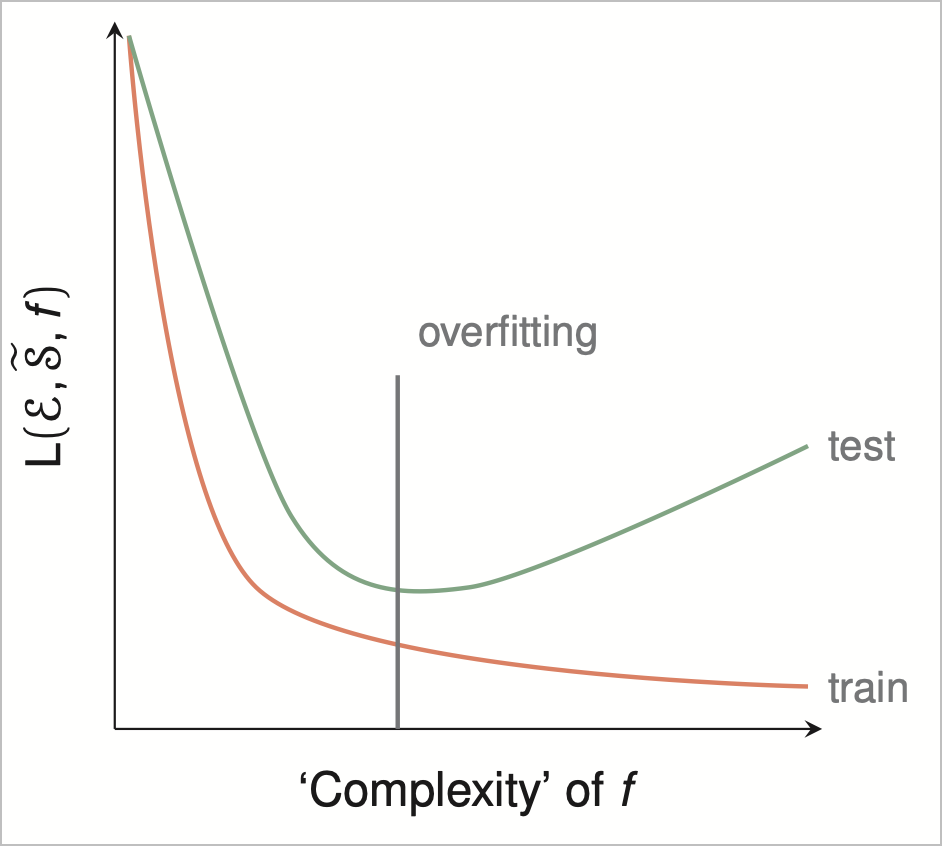
\includegraphics[width=0.4\textwidth]{learning-curve}
\end{figure}
\subsubsection{Bias-Variance Tradeoff}
We will never be able to completely reduce both effects in the absence of
complete population data. As we increase the complexity of the function class
the bias decreases but the variance increases as the hypothesis space grows.

The OLS analytical solution is given by the normal equations
$\mathbf{w}=\mathbf{X^{T}X}^{-1}\mathbf{X^{T}y}$. For $X\in \mathbb{R}^{n\times
k+1}$, $\mathbf{X^{T}X}$ is non-invertible if $k+1>n$ and we do not have a
unique solution.
\begin{remark}
  With a high enough degree polynomial we can always reduce our training error
  to zero.
\end{remark}
This can be remedied through regularisation, to manage model complexity.
Intuitively, this reduces potential for larger magnitude weights related to
higher complexity, and shrinks some of the weights towards zero.

\subsubsection{Regularisation}
In adoption of a Bayesian perspective, we model $\mathbf{w}$ as a random
variable, and the MAP solution to weight optimisation results in a regularised
objective. Depending on the distribution we select for $\mathbf{w}$, we may
derive ridge regression or LASSO.\\
With the PAC approach, we model a worst case probabilistic bound on the
generalised evaluation function $E_\mathcal{D}[L]$ given some function class.
We may also derive ridge regression or LASSO depending on which function class
is selected.

\subsection{Polynomial Regression --- Ridge Regression}
In Ridge Regression we optimise the empirical squared error loss function subject
to a constraint on $\left\lVert \mathbf{w} \right\rVert_2 \le t$.
\begin{itemize}
  \item \textbf{Representation} \[\mathcal{F}=\left\{ \mathbf{w\cdot x}|{\left\lVert \mathbf{w} \right\rVert}_2^2\le t \right\}\]
  \item \textbf{Evaluation} \[\frac{1}{2}\sum_{i=1}^{n} {(y^{(i)}-\mathbf{w\cdot x^{(i)}})}^{2}\]
  \item \textbf{Optimisation} \[\mathbf{w}_{OLS}=\argmin_\mathbf{w}\left\{
  \frac{1}{2}\sum_{i=1}^{n} {(y^{(i)}-\mathbf{w\cdot x^{(i)}})}^{2} +\frac{\lambda}{2}\sum_{i=1}^{m+1} {\left(w^{(i)}\right)}^2\right\}\]
\end{itemize}
Using Lagrange Multipliers, our optimisation problem is now as follows:
\[\nabla_\mathbf{w}\mathcal{L}(\mathbf{w},\lambda)=\mathbf{0}\]
\begin{align*}
  \text{subject to:}\quad&\left\lVert \mathbf{w} \right\rVert_2^2-t\le 0\\
                         &\lambda\ge 0\\
                         &\lambda\left( \left\lVert \mathbf{w} \right\rVert_2^2 -t \right) =0
\end{align*}
where $\mathcal{L}(\mathbf{w},\lambda)=\frac{1}{2}\sum_{i=1}^{n} \left( y^{(i)}-{\mathbf{w\cdot x}^{(i)}}^{2} \right) +\frac{\lambda}{2}\left( \left\lVert \mathbf{w} \right\rVert_2^2-t \right) $\\
If $\lambda=0$, the constraint is redundant, and the solution is the
non-regularised one. If $\lambda>0$, $\left\lVert \mathbf{w} \right\rVert_2
^2=t$ and we have an equality constraint.\\
For any given $t$, we can find the optimal $\lambda^{*}$ by solving for
$\nabla_\lambda \mathcal{L}(\mathbf{w},\lambda^{*})=\mathbf{0}$. Additionally,
$\mathcal{L}$ is convex w.r.t. $\mathbf{w}$ and we achieve optimum at
$\nabla_\mathbf{w} \mathcal{L}\left( \mathbf{w},\lambda \right) =\mathbf{0}$.
The new evaluation function then corresponds to this new objective:
\[\tilde{L}\left( \mathcal{E},\mathcal{S},\mathbf{f_w} \right)=\frac{1}{2}\left\lVert \mathbf{y-Xw} \right\rVert_2 ^{2}+\frac{\lambda}{2}\left\lVert \mathbf{w} \right\rVert_2 ^{2}\]
We can then solve for optimal $\mathbf{w}_{RR}$:
\begin{align*}
  \nabla_\mathbf{w}\tilde{L}=&\mathbf{X^{T}Xw-X^{T}y+\lambda w}\\
  \mathbf{w}_{RR}=&{\left( \mathbf{X^{T}X+\lambda I} \right) }^{-1}\mathbf{X^{T}y}.
\end{align*}
Since the Hessian $\mathcal{H}=\left( \mathbf{X^{T}X+\lambda I} \right) \succeq
0$ and is always invertible, $\tilde{L}$ is strictly convex and we obtain an
unique solution (with gradient descent).
\subsubsection{Complexity Tuning}
The regularisation parameter $\lambda$ and polynomial degree $k$ together are
complexity tuning hyperparameters:
\begin{itemize}
  \item High $\lambda$, low $k\implies$ low functional complexity $\implies$ underfitting
  \item Low $\lambda$, high $k \implies$ high functional complexity $\implies$ overfitting
\end{itemize}
However, in ridge regression, with a large number of weights, most of the
regularised weights can shrink to almost zero but will rarely reach zero. This
makes model interpretation difficult, especially with large number of
parameters.

\subsection{Polynomial Regression --- LASSO}
In LASSO, we optimise for the empirical squared error loss function, now
subject to a contraint on $\left\lVert \mathbf{w} \right\rVert_1 \le t$. This
has the effect of shrinking some weights more aggressively to zero.
\begin{itemize}
  \item \textbf{Representation} \[\mathcal{F}=\left\{ \mathbf{w\cdot x}|\left\lVert \mathbf{w} \right\rVert_1 \le t\right\}\]
  \item \textbf{Evaluation} \[\frac{1}{2}\sum_{i=1}^{n} {(y^{(i)}-\mathbf{w\cdot x^{(i)}})}^{2}\]
  \item \textbf{Optimisation} \[\mathbf{w}_{OLS}=\argmin_\mathbf{w}\left\{
    \frac{1}{2}\sum_{i=1}^{n} {(y^{(i)}-\mathbf{w\cdot x^{(i)}})}^{2}
+\frac{\lambda}{2}\sum_{i=1}^{m+1} {\left(w^{(i)}\right)}\right\}\]
\end{itemize}
However the evaluation function
\[\tilde{L}\left( \mathcal{E},\mathcal{S},\mathbf{f_w} \right)=\frac{1}{2}\sum_{i=1}^{n} {\left( \mathbf{y-Xw} \right)}^{T}\left( \mathbf{y-Xw} \right) +\frac{\lambda}{2}\left\lVert \mathbf{w} \right\rVert_1\] 
is non-differentiable and we cannot look for stationary points in order to
solve. We consider the subgradients:
\[\begin{cases}
  \frac{\partial L}{\partial w_j} +\frac{\lambda}{2} & \text{for } w_j>0\\
  \frac{\partial L}{\partial w_j} -\frac{\lambda}{2}& \text{for }w_j<0
\end{cases}\]
At $w_j=0$ we are at an optimal point if
\begin{align*}
  \frac{\partial L}{\partial w_j} +\frac{\lambda}{2}>0\quad & \text{and;}\quad \frac{\partial L}{\partial w_j} -\frac{\lambda}{2}<0\\
  \implies \frac{\lambda}{2}< &\frac{\partial L}{\partial w_j} <\frac{\lambda}{2}
\end{align*}
\subsubsection{Limitations}
\begin{itemize}
  \item When dealing with high dimensional data with few examples ($n<k+1$), LASSO
  selects at most $n$ variables before it saturates.
  \item With a highly correlated set of variables, LASSO tends to select one from the group and 
  ignore the others.
  \item LASSO optimisation is not necessarily strictly convex, and in general will not
  yield an unique solution.
\end{itemize}

\subsection{Polynomial Regression --- Elastic Net}
In Elastic Net Regularisation, Ridge Regression and LASSO is combined to remedy
various shortcomings.
\begin{itemize}
  \item \textbf{Representation} \[\mathcal{F}=\left\{ \mathbf{w\cdot x}|{\left\lVert \mathbf{w} \right\rVert}_2^2\le t_1 \wedge\left\lVert \mathbf{w} \right\rVert_1 \le t_2\right\}\]
  \item \textbf{Evaluation} \[\frac{1}{2}\sum_{i=1}^{n} {(y^{(i)}-\mathbf{w\cdot x^{(i)}})}^{2}\]
  \item \textbf{Optimisation} \[\mathbf{w}_{OLS}=\argmin_\mathbf{w}\left\{
  \frac{1}{2}\sum_{i=1}^{n} {(y^{(i)}-\mathbf{w\cdot x^{(i)}})}^{2} +\frac{\lambda}{2}\left( \alpha \sum_{i=1}^{m+1} {\left(w^{(i)}\right)}^2+(1-\alpha)\sum_{i=1}^{m+1} w^{(i)} \right) \right\}\]
  for some $0\le \alpha\le 1,\lambda\ge 0$
\end{itemize}
\subsubsection{Beneficial Properties}
\begin{itemize}
  \item Objective is strictly convex, and optimal Elastic Net weights are unique.
  \item The 1-norm term promotes sparsity.
  \item The 2-norm term promotes a grouping effect and removes the limitation
    on the number of selected variables.
\end{itemize}

\section{Classification}
In Classification we learn a mapping $f:\mathbb{R}^{m+1}\mapsto \left\{ 0,1,\ldots,k \right\}$,
drawn from a function class $\mathcal{f}$.

\begin{itemize}
  \item \textbf{Representation}
    \[f \in \mathcal{F}\] 
  \item \textbf{Evaluation}
    \[\text{Loss Measure: }\mathcal{E}\left(f\left(\mathbf{x}\right),y\right)=\mathbb{I}\left[ y\neq f(\mathbf{x}) \right]\] 
    \[\text{Generalisation Loss: }L(\mathcal{E},\mathcal{D}, f)=\mathbb{E}_\mathcal{D}\left[ \mathbb{I}\left[ \mathcal{Y}\neq f(\mathcal{X}) \right] \right]\] 
  \item \textbf{Optimisation}
    \[f^{*}=\argmin_{f \in \mathcal{F}}\left\{ \mathbb{E}_\mathcal{D}\left[ \mathbb{I}\left[ \mathcal{Y}\neq f(\mathcal{X}) \right] \right] \right\}\] 
\end{itemize}
\subsubsection{Classification Approaches}
\begin{figure}[h!]
  \centering
  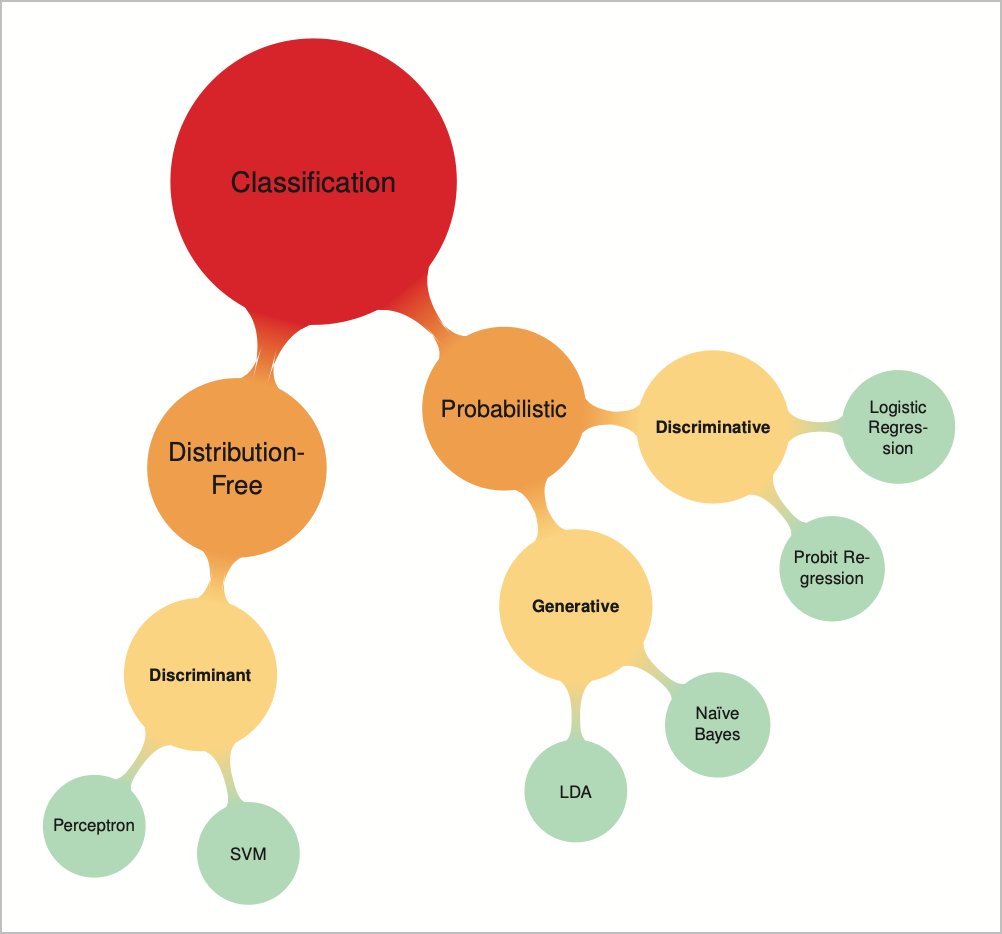
\includegraphics[width=0.5\textwidth]{classifications}
\end{figure}
\textbf{Distribution-free Classification} paradigm: We seek to learn the
classification boundary directly without probabilistic inference.\ e.g. PAC
approach where we seek to approximate $\mathbb{E}_\mathcal{D}\left[
  \mathbb{I}\left[ \mathcal{Y}\neq f(\mathcal{X}) \right] \right]$.
\textbf{Probabilitistic Classification} paradigm: The classification problem
reduces to an inference problem in which we learn the posterior output class
probability, each $p_\mathcal{Y}\left( y=1|\mathbf{x} \right) $characterising
an inhomogeneous Bernoulli distribution, for which we must parameterise a
distribution for each $\mathbf{x}\in dom(\mathcal{X})$\\
\textbf{Generative Classification}: To learn $p_\mathcal{Y}(y|\mathbf{x})$
indirectly by inferring the likelihood $p_\mathcal{X}(\mathbf{x}|y)$ and the
prior $p_\mathcal{Y}(y)$ for each class separately. Requires the most number of
parameters to learn, but allows us to learn $p_\mathcal{X}(\mathbf{x})$.\\
\textbf{Discriminative Classification}: To learn $p_\mathcal{Y}(y|\mathbf{x})$
directly. Less demanding in terms of number of parameters to learn, but is
inflexible, requiring re-running the lagorithm for changes of the loss
function and does not deal well with class imbalances.
\subsection{Baye's Optimal Classifier}
For the binary classification problem, we have Baye's Optimal Classifier
minimising misclassification loss: 
\[f*(\mathbf{x})=
\begin{cases}
  1&\text{if}\quad p_\mathcal{Y}(y=1|\mathbf{x})\ge 0.5\\
  0&\text{if}\quad p_\mathcal{Y}(y=1|\mathbf{x})< 0.5
\end{cases}\] 
\begin{proof}
  \begin{align*}
    f^{*}=&\argmin_{f \in \mathcal{F}}\left\{ \mathbb{E}_\mathcal{D}\left[ \mathbb{I}\left[ \mathcal{Y}\neq f(\mathcal{X}) \right] \right] \right\}\\
         =&\argmin_{f \in \mathcal{F}}\left\{ \sum_{y\in \left\{ 0,1 \right\}} \int p_\mathcal{Y}(y|x)p_\mathcal{X}(\mathbf{x})\mathbb{I}\left[ y\neq f(\mathbf{x}) \right] \,d\mathbf{x} \right\}\\
         =&\argmin_{f \in \mathcal{F}}\left\{ \sum_{y\in \left\{ 0,1 \right\}} \int p_\mathcal{Y}(y|x)p_\mathcal{X}(\mathbf{x})\left( f\left(\mathbf{x}\right) \left(1-y\right) +\left(1-f\left(\mathbf{x}\right)\right)y\right)  \,d\mathbf{x} \right\}\\
         =&\argmin_{f \in \mathcal{F}}\left\{ \int \left( p_\mathcal{Y}\left( y=1|\mathbf{x} \right) \left(1-f\left(\mathbf{x}\right)\right) +p_\mathcal{Y}\left( y=0|\mathbf{x} \right) f\left( \mathbf{x} \right)  \right) p_\mathcal{X}(\mathbf{x})\,d\mathbf{x}  \right\}\\
         =&\argmin_{f \in \mathcal{F}}\left\{ \int \left( p_\mathcal{Y}\left( y=1|\mathbf{x} \right) \left(1-f\left(\mathbf{x}\right)\right) +\left( 1-p_\mathcal{Y}\left( y=1|\mathbf{x} \right) \right)  f\left( \mathbf{x} \right)  \right) p_\mathcal{X}(\mathbf{x}) \,d\mathbf{x}  \right\}\\
         =&\argmin_{f \in \mathcal{F}}\left\{ \int \left( p_\mathcal{Y}\left( y=1|\mathbf{x} \right) +f\left( \mathbf{x} \right) \left( 1-2p_\mathcal{Y}\left( y=1|\mathbf{x} \right) \right) \right) p_\mathcal{X}(\mathbf{x}) \,d\mathbf{x}  \right\}
  \end{align*}
  Let $M(\mathbf{x})=p_\mathcal{Y}\left( y=1|\mathbf{x} \right) +f\left( \mathbf{x} \right) \left( 1-2p_\mathcal{Y}\left( y=1|\mathbf{x} \right) \right)$.\\
  We need to find function $f^{*}$ that is optimal for all $\mathbf{x}\in dom(\mathcal{X})$, 
  \[f^{*}(\mathbf{x})=\argmin_{f(\mathbf{x})}\left\{ M(\mathbf{x}) \right\}\]
  If $f^{*}(\mathbf{x})=1$ optimality implies:
  \begin{align*}
    1-p_\mathcal{Y}\left( y=1|\mathbf{x} \right) \le p_\mathcal{Y}\left( y=1|x \right) 
    p_\mathcal{Y}\left( y=1|\mathbf{x} \right) \ge 0.5
  \end{align*}\qed%
\end{proof}
\begin{remark}
  WLOG, we may consider the Bayes Optimal Classifier for Generative Classification as follows:
  \begin{align*}
    f^{*}(\mathbf{x})=&\argmax_{y\in \left\{ 0,1 \right\}}\left\{ p_\mathcal{Y}(y|\mathbf{x}) \right\}\\
    =&\argmax_{y\in \left\{ 0,1 \right\}}\left\{ \frac{p_\mathcal{X}\left( \mathbf{x}|y \right)P_\mathcal{Y}(y) }{\sum_{y\in \left\{ 0,1 \right\}} p_\mathcal{X}(\mathbf{X}|y)p_\mathcal{Y}(y)} \right\}\\
    =&\argmax_{y\in \left\{ 0,1 \right\}}\left\{ p_\mathcal{X}(\mathbf{x}|y)p_\mathcal{Y}(y) \right\}
  \end{align*}
\end{remark}
\subsection{Logistic Regression}
We seek to model $p_\mathcal{Y}(y=1|\mathbf{x})$ with a function
$f:\mathbb{R}^{m}\mapsto [0,1]$. In Logistic Regression, we assume that the probability can be
modelled by the logistic sigmoid:
\[S(x)=\frac{1}{1+e^{-\mathbf{w\cdot x}}}.\]
\begin{figure}[h!]
  \centering
  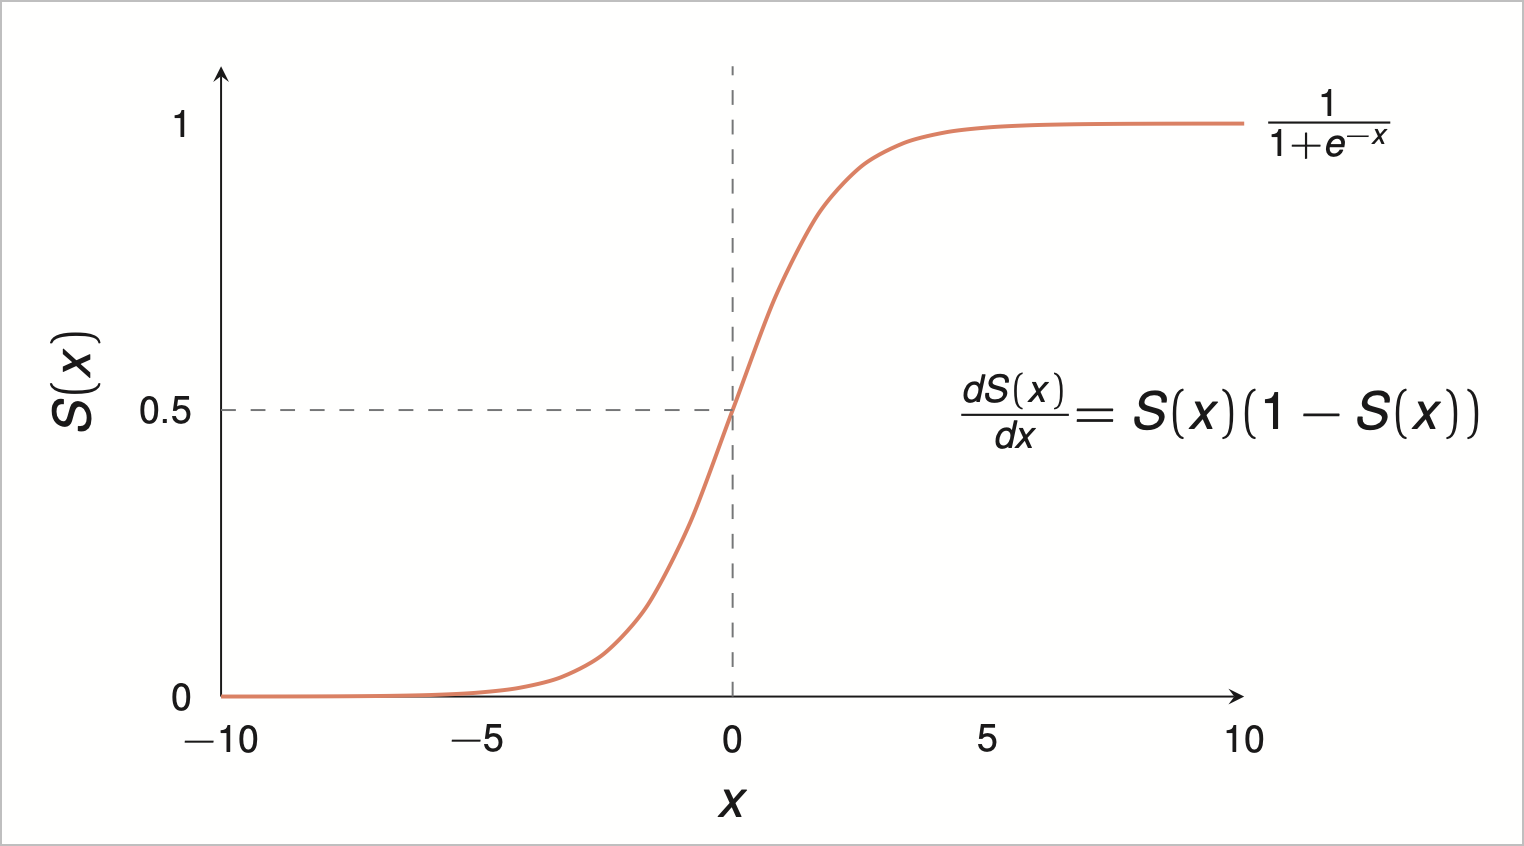
\includegraphics[width=0.6\textwidth]{logistic-sigmoid}
\end{figure}
\begin{itemize}
  \item \textbf{Representation}
    \[\mathcal{F}=\left\{ f_\mathbf{w}\left( \mathbf{x} \right) =\mathbb{I}\left[ p_\mathcal{Y}\left( y=1|\mathbf{x} \right) \ge 0.5 \right] | p_\mathcal{Y}\left( y=1|\mathbf{x} \right) =\frac{1}{1+e^{-\mathbf{w\cdot x}}},\mathbf{w}\in \mathbb{R}^{m+1} \right\}\] 
  \item \textbf{Evaluation}
      \[\mathcal{L}(\mathbf{w})= \sum_{i=1}^{n} y^{(i)}\mathbf{w\cdot
      x^{(i)}}-\ln\left( 1+e^{\mathbf{w\cdot x^{(i)}}} \right) \]
  \item \textbf{Optimisation}
    \[\mathbf{w}_{MLE}=\argmin_{\mathbf{w}}\left\{ \sum_{i=1}^{n} \ln\left( 1+e^{\mathbf{w\cdot x}^{(i)}} \right) - y^{(i)}\mathbf{w\cdot x}^{(i)}\right\}\] 
\end{itemize}
Rearranging, we have
\begin{align*}
  p_\mathcal{Y}\left( y=1|\mathbf{x} \right) =&\frac{1}{1+e^{-\mathbf{w\cdot x}}}\\
  e^{-\mathbf{w\cdot x}}=&\frac{1}{p_\mathcal{Y}(y=1|\mathbf{x})}-1\\
  \mathbf{w\cdot x}=&\ln\left( \frac{p_\mathcal{Y}(y=1|\mathbf{x})}{1-p_\mathcal{Y}(y=1|\mathbf{x})} \right)\\
  =&logit(p_\mathcal{Y}(y=1|\mathbf{x}))
\end{align*}
\begin{remark}
$\mathbf{w\cdot x}=0$ defines a linear discriminant separating hyperplane.
\end{remark}
\subsubsection{Evaluation}
\begin{multicols}{2}
  [With the logistic regression model, we have the following:]
   \begin{align*}
    \mathcal{Y}\left( y=1|\mathbf{x} \right)=\frac{1}{1+e^{-\mathbf{w\cdot x}}}\\\\
   \end{align*}
   \begin{align*}
     p_\mathcal{Y}\left( y=0|\mathbf{x} \right)=&\frac{e^{-\mathbf{w\cdot x}}}{1+e^{-\mathbf{w\cdot x}}}\\
     =&\frac{1}{1+e^{\mathbf{w\cdot x}}}
   \end{align*}
\end{multicols}
We can then derive the Cross-Entropy loss function for logistic regression:
\begin{align*}
\mathcal{L}(\mathbf{w})=&\ln\left( \prod_{i=1}^{n} p_\mathcal{Y}\left( y^{(i)}|\mathbf{x}^{(i)} \right)   \right) \\
=&\sum_{i=1}^{n} \ln\left( p_\mathcal{Y}\left( y^{(i)}|\mathbf{x}^{(i)} \right)  \right) \\
=&\sum_{i=1}^{n} y^{(i)}\ln\left( p_\mathcal{Y}\left( y^{(i)}=1|\mathbf{x}^{(i)} \right)  \right) + \left( 1-y^{(i)}\right) \ln\left( p_\mathcal{Y}\left( y^{(i)}=0|\mathbf{x}^{(i)} \right)  \right)  \\
=&\sum_{i=1}^{n} \ln\left( p_\mathcal{Y}\left( y^{(i)}=0|\mathbf{x}^{(i)} \right)  \right) + y^{(i)} \ln\left( \frac{p_\mathcal{Y}\left( y^{(i)}=1|\mathbf{x}^{(i)} \right)}{p_\mathcal{Y}\left( y^{(i)}=0|\mathbf{x}^{(i)} \right)} \right)  \\
=&\sum_{i=1}^{n} y^{(i)}\mathbf{w\cdot x^{(i)}}-\ln\left( 1+e^{\mathbf{w\cdot x^{(i)}}} \right) 
\end{align*}
Hence we seek $\mathbf{w}_{MLE}$:
\[\mathbf{w}_{MLE}=\argmin_{\mathbf{w}}\left\{ \sum_{i=1}^{n} \ln\left( 1+e^{\mathbf{w\cdot x}^{(i)}} \right) - y^{(i)}\mathbf{w\cdot x}^{(i)}\right\}\] 
\subsubsection{Motivation}
We assume some latent random variable $\mathcal{Y}^{*}$ such that
$y^{*}=\mathbf{w\cdot x}+\epsilon$ where $\epsilon\sim Logistic(0,1)$. Then
\[\varepsilon\sim Logistic(\mu,s)\quad\text{where:}\quad\mu\in \mathbb{R},s>0.\]
\begin{definition}[Logistic Distribution]
  The Logistic Distribution has the characteristic pdf:
\[f_\epsilon\left( \varepsilon;\mu,s \right) =\frac{e^{-\frac{\varepsilon-\mu}{s}}}{s{\left( 1+e^{-\frac{\varepsilon-\mu}{s}} \right) }^{2}}.\] 
\[E_\mathcal{D}[\epsilon]=\mu.\] 
\[P(\epsilon<z)=\frac{1}{1+e^{-\frac{z-\mu}{s}}}.\] 
\end{definition}
We link a latent variable outcome to an output assuming the classification
model:
\[y^{(i)}=\begin{cases}
  1&\text{if }\quad y^{*(i)}\ge 0\\
  0&\text{if }\quad y^{*(i)}< 0\\
\end{cases}.\]
\begin{align*}
  p_\mathcal{Y}\left( y^{(i)}=1|\mathbf{x}^{(i)} \right)=&P\left(\mathcal{Y}^{*(i)}\ge 0|\mathbf{x}^{(i)}\right)\\
  =&P\left( \mathbf{w\cdot x}^{(i)}+\varepsilon^{(i)} \ge 0\right)\\
  =&1-\frac{1}{1+e^{\mathbf{w\cdot x}^{(i)}}}\\
  =&\frac{e^{\mathbf{w\cdot x}^{(i)}}}{1+e^{\mathbf{w\cdot x}^{(i)}}}\\
  =&\frac{1}{1+e^{-\mathbf{w\cdot x}^{(i)}}}\\
\end{align*}
\subsubsection{Optimisation}
However, the $\mathbf{w}_{MLE}$ we seek has no analytic solution. We may apply
a numerical technique to optimise. This optimisation is a convex problem, hence the
local optimum found would also be a global optimum.
\[\nabla_\mathbf{w}^{2} \mathcal{L}\ge 0.\] 
\begin{proof}
  \begin{align*}
    \nabla_\mathbf{w} (-y\mathbf{w\cdot x})=&-y\mathbf{x}\\
    \nabla_\mathbf{w}^{2} (-y\mathbf{w\cdot x})=&\mathbf{0}\\
    \implies \mathcal{H}=&\mathbf{0}
  \end{align*}
  $-y\mathbf{w\cdot x}$ is convex.\\
  \begin{align*}
  \nabla_\mathbf{w}\left(  \ln(1+e^{\mathbf{w\cdot x}}) \right)=&\frac{e^{\mathbf{w\cdot x}}}{1+e^{\mathbf{w\cdot x}}} \mathbf{x}\\
  \frac{\partial \ln(1+e^{\mathbf{w\cdot x}})}{\partial w_i} =&\frac{e^{\mathbf{w\cdot x}}}{1+e^{\mathbf{w\cdot x}}} x_i\\
  \frac{\partial^{2} \ln(1+e^{\mathbf{w\cdot x}})}{\partial w_i\partial w_j} =&\frac{e^{\mathbf{w\cdot x}}}{{(1+e^{\mathbf{w\cdot x}})}^{2}} x_i x_j\\
  \mathcal{H}=&\frac{e^{\mathbf{w\cdot x}}}{{(1+e^{\mathbf{w\cdot x}})}^{2}}\mathbf{xx}^{T}\\
  \implies\mathcal{H}\succeq&0
  \end{align*}
  The objective is convex.\qed%
\end{proof}
\subsubsection{Linearly Separable Data}
Consider that the training data is linearly separable. Consider the objective
function for some $w=c\tilde{w}, c>0$:
\[\sum_{i=1}^{n} \ln\left( 1+e^{c\mathbf{\tilde{w}\cdot x}^{(i)}} \right)-y^{(i)}c\mathbf{\tilde{w}\cdot x}^{(i)}\] 
Taking the derivative with respect to $c$, we have:
 \[\sum_{i=1}^{n} \mathbf{\tilde{w}\cdot x}^{(i)}\left( \frac{e^{c\mathbf{\tilde{w}\cdot x}^{(i)}}}{1+e^{c\mathbf{\tilde{w}\cdot x}^{(i)}}}-y^{(i)} \right).\]
Since the data is well classified, there always exists a $\tilde{w}$ such that
the objective has a negative derivative with respect to $c$, and gradient
descent will cause $c$ to grow without bound. The sigmoid function approaches
a Heaviside function. This is a case of overfitting and can be circumvented
through regularisation:
\[\sum_{i=1}^{n} \ln\left( 1+e^{c\mathbf{\tilde{w}\cdot x}^{(i)}} \right)-y^{(i)}c\mathbf{\tilde{w}\cdot x}^{(i)}+\lambda c^{2}\left\lVert \mathbf{\tilde{w}} \right\rVert_2^{2} \]
We may discern a unique stationary point with respect to $c$ with the
derivative, using the addition of a Ridge Regulariser. Apart from the linearly
separable non-regularised case, Logistic Regression in general leads to unique
solutions.
\subsubsection{Multinomial Logistic Regression}
Supposing we have $k$ classes such that $y\in \left\{ 1,\ldots,k \right\}$, the Bayes
Optimal Classifier becomes:
\[f^{*}(\mathbf{x})=\argmax_{y\in \left\{ 1,\ldots,k \right\}}\left\{ p_\mathcal{Y}(y|\mathbf{x}) \right\}.\] 
The model is now defined using the softmax function, and we seek to learn an
inhomogeneous multinomial distribution:
\[p_\mathcal{Y}(y=k|\mathbf{x})=\frac{e^{\mathbf{w}_j\cdot \mathbf{x}}}{\sum_{j=1}^{k} e^{\mathbf{w}_j\cdot\mathbf{x}}}.\] 
The maximum likelihood solution will now make use of the multinomial cross
entropy which results in a convex optimisation problem.

\subsection{Naïve Bayes}
In Naïve Bayes, we simplify the likelihood by assuming the conditional
independence assumption of the input attributes given $\mathcal{Y}$:
\[p_\mathcal{X}(\mathbf{x}|y)=\prod_{i=1}^{m} p_\mathcal{X_i} (x_i|y)\] 
Supposing $\mathcal{Y}$ is a Bernoulli random variable,
$y\sim Bern(\theta_y)$. We find the log-likelihood function:
\begin{align*}
\mathcal{L}\left( \theta \right) =& \ln\left( \prod_{i=1}^{n} p_\mathcal{Y}\left( y^{(i)};\theta_y \right) \right)\\
=&\sum_{i=1}^{n} \ln\left( p_\mathcal{Y}\left( y^{(i)};\theta_y \right)  \right)\\
=&\sum_{i=1}^{n} y^{(i)}\ln\theta_y+\left(1-y^{(i)}\right)\ln\left( 1-\theta_y \right) 
\end{align*}
Hence we seek $\theta_{yMLE}$ such that:
\[\theta_{yMLE}=\argmax_{\theta_y}\left\{ \sum_{i=1}^{n} y^{(i)}\ln\theta_y+\left(1-y^{(i)}\right)\ln\left( 1-\theta_y \right) \right\}\] 
Taking the derivative and setting to 0, we have:
\begin{align*}
\nabla_{\theta_y}L=&\sum_{i=1}^{n} \frac{y^{(i)}}{\theta_y}-\frac{(1-y^{(i)})}{1-\theta_y}\\
\implies\theta_{yMLE}=&\frac{n_1}{n}
\end{align*}
\subsubsection{Categorical Naïve Bayes}
Suppose that the features $x_i$ are discrete-valued and take $m_i$ different
values, such that each outcome $x_i$ is taken from the set ${\left\{ x_{ij}
\right\}}_{j=1}^{m_i}$
\begin{itemize}
  \item \textbf{Representation}
      \[\mathcal{F}=\left\{ f_{\theta_y,\left\{ \theta_{ijk} \right\}} (\mathbf{x})=\argmax_{y\in \left\{ 0,1 \right\}} \left\{ p_\mathcal{Y}(y)\prod_{i=1}^{m} p_\mathcal{X_i} (x_i|y) \right\} \mid p_\mathcal{Y}(y=1)=\theta_y,{\left\{ p_\mathcal{X_i}(x_{ij}|k)=\theta_{ijk} \right\}}^{m,m_i,1}_{i=1,j=1,k=0} \right\}.\] 
  \item \textbf{Evaluation}
    \[\ln\left( L(\theta_y) \right)\quad\text{and}\quad {\left\{ \ln\left( L\left( \theta_{ik} \right)  \right) \right\}}^{m,1}_{i=1,k=0}\] 
  \item \textbf{Optimisation}
    \[\theta_{yMLE}=\frac{n_1}{n}\quad\text{and}\quad {\left\{\theta_{ijkMLE}=\frac{n_{ijk}}{n_k}\right\}}^{m,m_i,1}_{i=1,j=1,k=0}\] 
\end{itemize}
Each $(x_i|y=k)$ is a categorical random variable, of which we seek to
parameterise its categorical distribution.
\begin{definition}[Categorical Distribution]
  The Categorical Distribution is a generalisation of the Bernoulli
  Distribution with more than 2 discrete outcomes ($m_i$ discrete outcomes):
  \[(\mathbf{x}_i|y=k)\sim Categorical(\Theta_{ik})\]
  \[\Theta_{ik}\text{ has elements }{\left\{ \theta_{ijk} \right\}}_{j=1}^{m_i}\]
  \[p_\mathcal{X_i}\left( \mathcal{X}_i=x_{ij}|y=k;\Theta_{ik} \right)=\theta_{ijk} \] 
  \[\sum_{j=1}^{m_i} \theta_{ijk}=1\]
\end{definition}
By forming the log-likelihood, and performing a constrained optimisation of the
resulting function, we can obtain:
\[\theta_{ijkMLE}=\frac{n_{ijk}}{n_k}.\]
where $n_{ijk}$ is the number of training points for which the $i$-th attribute
belongs to the $j$-th category and $\mathcal{Y}=k$, and $n_k$ is the number of
training points of which $\mathcal{Y}=k$.
\subsubsection{Additive Smoothing}
To remedy the problem such that any category does not contain any instances,
and prevent a case of overfitting where we estimate the probability of the
event to be zero, we may utilise additive smoothing, adjusting the MLE
estimates such that:
\[\theta_{ijk}=\frac{n_{ijk}+\alpha}{n_k+\alpha J}.\] 
\[\theta_y=\frac{n_1+\alpha}{n+\alpha K}.\]
where:
\begin{itemize}
  \item $J=$ \# of distinct values outcomes of $\mathcal{X}_i$ can take ($m_i$ in this case)
  \item $K=$ \# of distinct values outcomes of $\mathcal{Y}$ can take
  \item $\alpha=$ the strength of smoothing
\end{itemize}
\subsubsection{Gaussian Naïve Bayes}
Suppose that the features $x_i\in \mathbb{R}$ are continuous valued, such that
each $(\mathcal{X}_i|y=k)$ is a Gaussian random variable, $(x_i|y=k)\sim
\mathcal{N}\left( \mu_{ik},\sigma_{ik} \right) $. We then find the
log-likelihood:
\begin{align*}
  \mathcal{L}(\theta)=&\ln\left( \prod_{j=1}^{n_k} \frac{1}{\sqrt{2\pi\sigma_{ik}^{2}}}\exp\left(-\frac{{(x_i^{(j)}-\mu_{ik})}^{2}}{2\sigma_{ik}^{2}}\right)  \right) \\
  =&-n_k \ln\sigma_{ik}-\sum_{j=1}^{n_k} \left(-\frac{{(x_i^{(j)}-\mu_{ik})}^{2}}{2\sigma_{ik}^{2}}\right)+const.
\end{align*}
We can optimise the log-likelihood with:
\[\mu_{ikMLE}=\sum_{j=1}^{n_k} \frac{x_i^{(j)}}{n_k}.\] 
\[\sigma_{ikMLE}^{2}=\frac{1}{n_k}\sum_{j=1}^{n_k} {(x_i^{(j)}-\mu_{ik})}^{2}.\] 
\begin{itemize}
  \item \textbf{Representation}
    \[\mathcal{F}=\left\{ f_{\theta_y,\left\{ \theta_{ijk} \right\}} (\mathbf{x})=\argmax_{y\in \left\{ 0,1 \right\}} \left\{ p_\mathcal{Y}(y)\prod_{i=1}^{m} \mathcal{N}\left(X_i;\mu_{ik},\sigma_{ik}\right) \right\} \mid p_\mathcal{Y}(y=1)=\theta_y,{\left\{ \mu_{ik}\in \mathbb{R},\sigma_{ik}>0 \right\}}^{m,1}_{i=1,k=0} \right\}.\] 
  \item \textbf{Evaluation}
    \[\ln\left( L(\theta_y) \right)\quad\text{and}\quad {\left\{ \ln\left( L\left( \mu_{ik},\sigma_{ik}\right)  \right) \right\}}^{m,1}_{i=1,k=0}\] 
  \item \textbf{Optimisation}
    \[\theta_{yMLE}=\frac{n_1}{n}\quad\text{and}\quad {\left\{\mu_{ikMLE}=\sum_{j=1}^{n_k} \frac{x_i^{(j)}}{n_k},\sigma_{ikMLE}=\frac{1}{n_k}\sum_{j=1}^{n_k} {(x_i^{(j)}-\mu_{ik})}^{2} \right\}}^{m,1}_{i=1,k=0}\] 
\end{itemize}
\begin{remark}
  GNB results in a similar form of linear discriminant as LR\@. However, they do
  not result in the same classifier, as GNB makes certain model assumptions
  that defines a dependence between $w_0$ and $w_i$.
\end{remark}

\subsection{Comparisons}
Using a generative classifier requires learning more parameters than
discriminative classifiers, but the generative approach is often intractable
and require certain model assumptions (e.g. Conditional Independence). Since LR
makes fewer model assumptions than a generative one such as NB, LR is
considered more robust and less sensitive to modelling choices than NB, but NB
requires less data for similar levels of convergence.

\section{Model Selection}
In Model Selection, we seek to choose the best hyperparameter / learning
algorithm / model for a particular problem. We are primarily concerned with
ranking a set of models, rather than estimating the performance of a particular
model.
\subsubsection{Measures for Performance}
The measure of performance we are ultimately interested in is \textbf{Generalisation Loss}:
\[\mathbb{E}_\mathcal{D}\left[ \mathcal{E}\left( f(\mathbf{\mathcal{X}}) ,\mathcal{Y}\right) \right].\] 
This cannot be directly measured, and empirical test set loss,
$\mathbb{E}_\mathcal{S_{Test}}\left[ \mathcal{E}\left( f(\mathbf{\mathcal{X}})
,\mathcal{Y}\right) \right]$ can act as a reasonable estimator (but not for
model selection). Empirical Training Set Loss cannot be used as well, as it
will lead to overfitting.\\
Hence, Empirical Risk Minimisation alone is not adequate to perform model
selection.

\subsection{Validation Techniques}
We seek to estimate the generalisation loss through a \textbf{Validation Set
Loss}. We split the training data into three sets:
\begin{itemize}
  \item Training: To train each possible model
  \item Validation: To select the `best' model
  \item Test: To assess the performance of that model
\end{itemize}
\begin{figure}[h!]
  \centering
  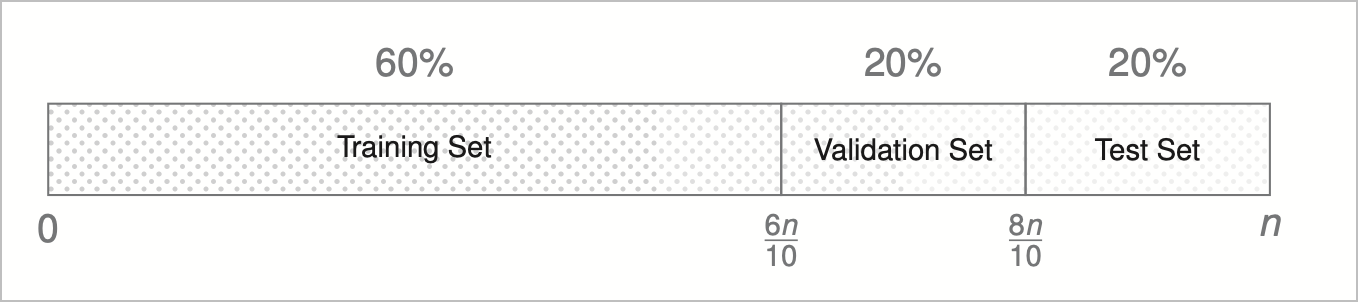
\includegraphics[width=0.8\textwidth]{validation}
\end{figure}
\subsubsection{Validation Loss Bound}
Applying the Hoeffding's Inequality to i.i.d. $\mathcal{Z}_i=\mathbb{I}\left[ \mathcal{Y}^{(i)}\neq f\left( \mathcal{\mathbf{X}}^{(i)} \right) \right]$:
\[P\left( E_\mathcal{D}\left[ \mathbb{I}\left[ \mathcal{Y}\neq f\left( \mathcal{\mathbf{X}} \right)  \right] \right] \ge \frac{1}{n_v}\sum_{i=1}^{n_v} \mathbb{I}\left[ y^{(i)}\neq f(\mathbf{x}^{(i)}) \right] + \epsilon\right)\le e^{-2n_v\epsilon^{2}}.\] 
\[P\left( E_\mathcal{D}\left[ \mathbb{I}\left[ \mathcal{Y}\neq f\left( \mathcal{\mathbf{X}} \right)  \right] \right] \ge E_{S_v} \left[ \mathbb{I}\left[ y^{(i)}\neq f(\mathbf{x}^{(i)}) \right] \right] + \epsilon\right)\le e^{-2n_v\epsilon^{2}}.\] 
Let $\delta=e^{-2n_v\epsilon^{2}}\implies\epsilon=\sqrt{\frac{\ln\left( \frac{1}{\delta} \right) }{2n_v}}$.
\[P\left( E_\mathcal{D}\left[ \mathbb{I}\left[ \mathcal{Y}\neq f\left( \mathcal{\mathbf{X}} \right)  \right] \right] < E_{S_v} \left[ \mathbb{I}\left[ \mathcal{Y}\neq f(\mathcal{\mathbf{X}}) \right] \right] + \sqrt{\frac{\ln\left( \frac{1}{\delta} \right) }{2n_v}}\right)> (1-\delta).\] 
That is, with probability greater than $(1-\delta)$, we state that:
\[L(\mathcal{E}, \mathcal{D}, f)\le L(\mathcal{E}, \mathcal{S}_v, f)+\sqrt{\frac{\ln\left( \frac{1}{\delta} \right) }{2n_v}}.\] 
Using the Union Bound, we can show that a bound holds for all members in a finite hypothesis class
$\mathcal{F}$:
Let $A,B$ be the events:
\[A=\left\{ L(\mathcal{E}, \mathcal{D}, f^{A})\le L(\mathcal{E}, \mathcal{S}_v, f^{A})+\sqrt{\frac{\ln\left( \frac{1}{\delta'} \right) }{2n_v}} \right\}.\] 
\[B=\left\{ L(\mathcal{E}, \mathcal{D}, f^{B})\le L(\mathcal{E}, \mathcal{S}_v, f^{B})+\sqrt{\frac{\ln\left( \frac{1}{\delta'} \right) }{2n_v}} \right\}.\] 
We have $P(A)=P(B)<\delta'$.
\begin{remark}
  \[P(\neg A\wedge\neg B)\ge 1-(P(A) + P(B)).\]
\end{remark}
Combining these, $\forall f \in \left\{ f^{A},f^{B} \right\}$:
\[P\left( L(\mathcal{E}, \mathcal{D}, f)\le L(\mathcal{E}, \mathcal{S}_v, f)+\sqrt{\frac{\ln\left( \frac{1}{\delta'} \right) }{2n_v}} \right)\ge 1-2\delta'.\] 
Let $\delta=2\delta'$, and we have:
\[P\left( L(\mathcal{E}, \mathcal{D}, f)\le L(\mathcal{E}, \mathcal{S}_v, f)+\sqrt{\frac{\ln\left( \frac{2}{\delta} \right) }{2n_v}} \right)\ge 1-\delta.\] 
In general, $\forall f\in\mathcal{F}$:
\[P\left( L(\mathcal{E}, \mathcal{D}, f)\le L(\mathcal{E}, \mathcal{S}_v, f)+\sqrt{\frac{\ln\left( \frac{\left| {\mathcal{F}} \right|}{\delta} \right) }{2n_v}} \right)\ge 1-\delta.\] 
The validation is a good estimate provided $\mathcal{F}$ is not too large, and
$n_v$ is not too small. Otherwise, the validation and generalisation losses
will vary further as we begin to overfit.

\subsection{Cross Validation}
To retain most of our data for training, we perform validation while still
maintaining the training data set, by spliting the training data into $k$
folds. The learning algorithm is run $k$ times for each model, each time using
all the folds but one as the training set, and the remaining fold as the
validation set.
\begin{figure}[h!]
  \centering
  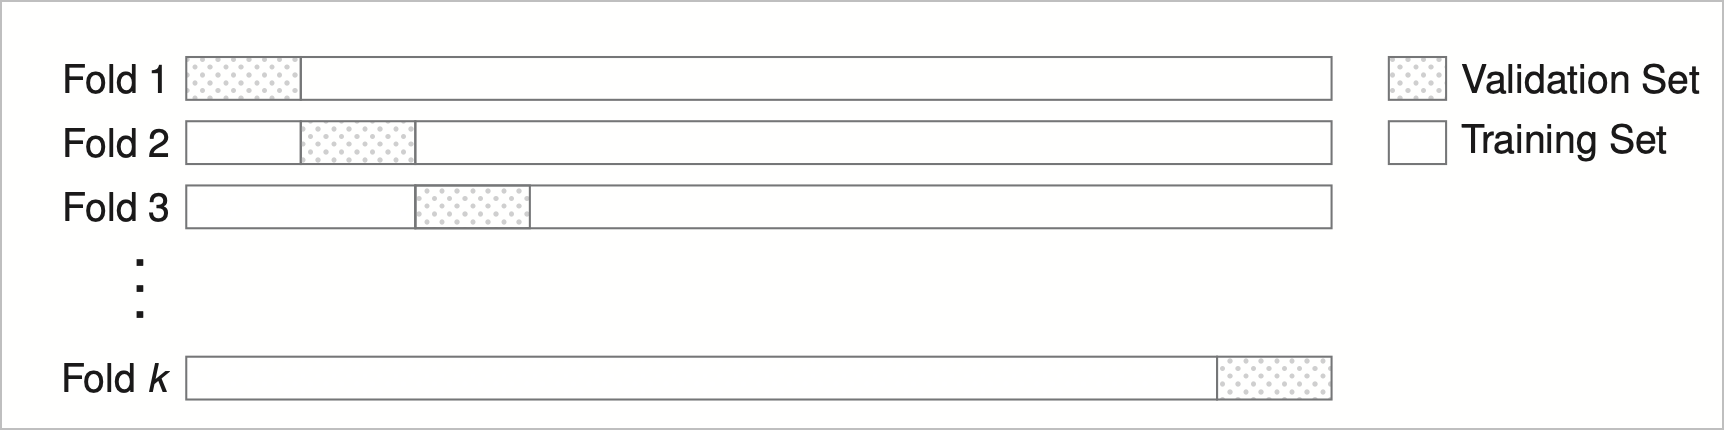
\includegraphics[width=0.8\textwidth]{cross-validation}
\end{figure}
The cross validation loss is the performance averaged across all $k$ folds:
\[L_{{CV}_k}\left( \mathcal{E}, \mathcal{S}, f \right) =\frac{1}{k}\sum_{i=1}^{k} L_{\mathcal{S}\backslash\mathcal{S}_k}\left( \mathcal{E},\mathcal{S}\backslash\mathcal{S}_i ,f \right).\] 
\subsubsection{$k$ selection}
$k=n$ is known as the Leave One Out cross validation, maximising the training
set for each fold, is computation expensive, and fails to give a good estimate
of the generalisation loss.\\
Empirical analysis suggests $k=5$ or $10$.
\subsubsection{Limitations}
There is not yet a rigorous understanding of why cross validation works well,
and in certain circumstances should be treated with care.
\begin{example}[Time Series Data]
  Requires sequential cross validation, due to similar neighbouring points.
\end{example}

\subsection{PAC Approach}
In the PAC (Probably Approximately Correct) approach, we formulate a
probabilistic `worst-case' bound using the empirical training loss and some
complexity penalty (taking into account $\left| \mathcal{F} \right| $). We then
perform based on the model that provides the tightest bound.\\\\
We obtain these bounds using the Uniform Convergence approach, by first seeking
a finite sample concentration inequality independent of $\mathcal{D}$ to one
function $f$, then applying it uniformly across all $f \in \mathcal{F}$ via
Union Bound or other measure of functional complexity.\\\\
We consider a probability of success $(1-\delta)$, an approximation loss target
$\epsilon$, and a data generating process $\mathcal{D}$.

\subsubsection{Consistent Learner}
For a consistent learning algorithm that only outputs hypotheses consistent
with the training data ($E_\mathcal{S}\left[
\mathcal{E}(f(\mathcal{X}),\mathcal{Y}) \right]=0$), for
$0<\epsilon<1,0<\delta<1$ and a particular $f \in \mathcal{F}\wedge
E_\mathcal{D}\left[ \mathcal{E}\left( f(\mathcal{\mathbf{X}}),\mathcal{Y}
\right) \right]>\epsilon$:
\[P(f\text{ is consistent with 1 training ex.})<(1-\epsilon)<e^{-\epsilon}.\] 
\[P(f\text{ is consistent with $n$ training ex.})<{(1-\epsilon)}^{n}<e^{-\epsilon n}.\] 
Applying the Union Bound $\forall f \in \mathcal{F}$, we obtain:
\[P\left( E_\mathcal{D}\left[ \mathcal{E}\left( f(\mathbf{X}),\mathcal{Y} \right) \right]>\epsilon, \text{ for at least one $f \in \mathcal{F}$}\right)<\left| \mathcal{F} \right|e^{-\epsilon n}.\] 
\begin{theorem}[PAC Bound: Finite $\mathcal{F}$, Consistent Learner]
  For all $0<\epsilon<1$, $0<\delta<1$, all data generating distributions $\mathcal{D}$, with
  probability of at least $(1-\delta)$:
  \[\forall f \in \mathcal{F}\quad E_\mathcal{D}\left[ \mathcal{E}\left( f(\mathbf{\mathcal{X}}),\mathcal{Y} \right) \right]\le \frac{1}{n}\ln\left( \frac{\left| \mathcal{F} \right|}{\delta}  \right).\] 
\end{theorem}

\subsubsection{Agnostic Learner}
For a learning algorithm which is not restricted in the hypotheses:
Applying the Hoeffding's Inequality to i.i.d. $\mathcal{Z}_i=\mathbb{I}\left[ \mathcal{Y}^{(i)}\neq f\left( \mathcal{\mathbf{X}}^{(i)} \right) \right]$:
\[P\left( E_\mathcal{D}\left[ \mathbb{I}\left[ \mathcal{Y}\neq f\left( \mathcal{\mathbf{X}} \right)  \right] \right] \ge \frac{1}{n}\sum_{i=1}^{n} \mathbb{I}\left[ y^{(i)}\neq f(\mathbf{x}^{(i)}) \right] + \epsilon\right)\le e^{-2n\epsilon^{2}}.\] 
\[P\left( E_\mathcal{D}\left[ \mathbb{I}\left[ \mathcal{Y}\neq f\left( \mathcal{\mathbf{X}} \right)  \right] \right] \ge E_{S} \left[ \mathbb{I}\left[ \mathcal{Y}\neq f(\mathcal{\mathbf{X}}) \right] \right] + \epsilon \right)> e^{-2n\epsilon^{2}}.\] 
Similarly, we applying the Union Bound to obtain:
\[P\left( E_\mathcal{D}\left[ \mathbb{I}\left[ \mathcal{Y}\neq f\left( \mathcal{\mathbf{X}} \right)  \right] \right] \ge E_{S} \left[ \mathbb{I}\left[ \mathcal{Y}\neq f(\mathcal{\mathbf{X}}) \right] \right] + \epsilon\text{, for at least one }f \in \mathcal{F}\right)\le \left| \mathcal{F} \right| e^{-2n\epsilon^{2}}.\] 
\begin{theorem}[PAC Bound: Finite $\mathcal{F}$, Agnostic Learner]
  For all $0<\epsilon<1$, $0<\delta<1$, all data generating distributions $\mathcal{D}$, with
  probability of at least $(1-\delta)$:
\[\forall f \in \mathcal{F}\quad E_\mathcal{D}\left[ \mathbb{I}\left[ \mathcal{Y}\neq f\left( \mathcal{\mathbf{X}} \right)  \right] \right] \le E_{S} \left[ \mathbb{I}\left[ \mathcal{Y}\neq f(\mathcal{\mathbf{X}}) \right] \right] + \sqrt{\frac{1}{2n}\ln\left( \frac{\left| \mathcal{F} \right|}{\delta}  \right) }\] 
\end{theorem}

\subsubsection{Infinite $\mathcal{F}$}
\begin{theorem}[PAC Bound: Infinite $\mathcal{F}$, Agnostic Learner]
  For all $0<\epsilon<1$, $0<\delta<1$, all data generating distributions $\mathcal{D}$, with
  probability of at least $(1-\delta)$:
\[\forall f \in \mathcal{F}\quad E_\mathcal{D}\left[ \mathbb{I}\left[ \mathcal{Y}\neq f\left( \mathcal{\mathbf{X}} \right)  \right] \right] \le E_{S} \left[ \mathbb{I}\left[ \mathcal{Y}\neq f(\mathcal{\mathbf{X}}) \right] \right] + 2\mathbb{R}\left( \mathcal{F}\circ\mathcal{S} \right) + 4\sqrt{\frac{2}{n}\ln\left( \frac{4}{\delta}  \right) }\] 
where $\mathbb{R}\left( \mathcal{F}\circ\mathcal{S} \right)$ denotes the Rademacher complexity of $\mathcal{F}\circ\mathcal{S}={\left\{ f(\mathbf{x}^{(i)})|f \in \mathcal{F} \right\}}_{i=1}^{n}$
\end{theorem}

\subsubsection{Advantages and Limitations}
The PAC approach is not limited to misclassification loss, but to a variety of
other loss functions. It allows comparison with training data alone while
avoiding overfitting.\\

However, the bounds are often loose, and are poor estimators of generalisation
loss, and tend to underperform cross validation.

\section{Clustering}
In Clustering, we seek to learn groups or clusters from our input data, and in
so doing assign each instance to a cluster. Intuitively, we group objects such
that similar objects end up in the same group.
\subsubsection{Measures of Similarity}
\begin{figure}[h!]
  \centering
  \raisebox{-0.5\height}{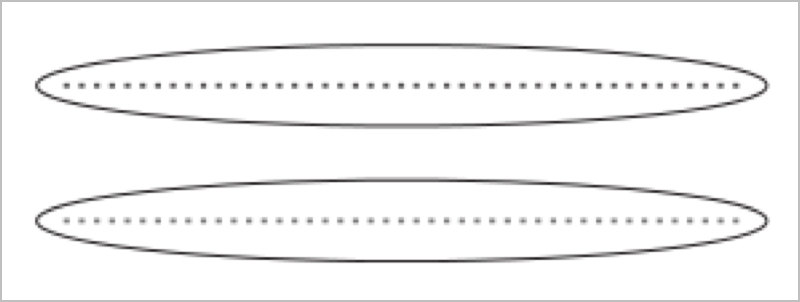
\includegraphics[width=0.4\textwidth]{transitivity}}
  \hspace*{.2in}
  \raisebox{-0.5\height}{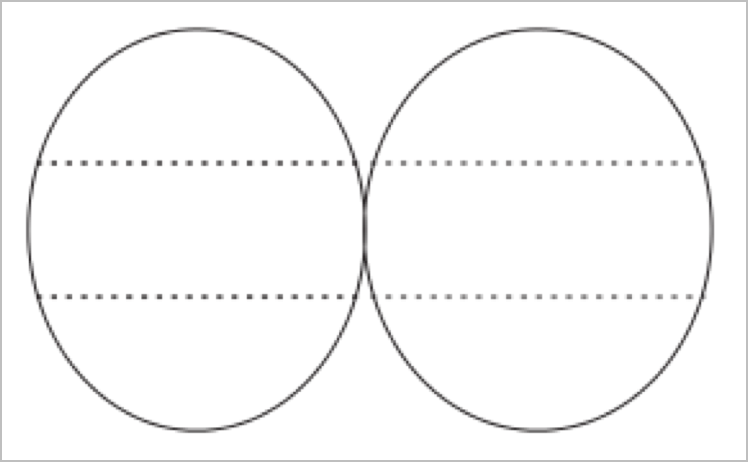
\includegraphics[width=0.4\textwidth]{proximity}}
\end{figure}
As measures of similarity, we can consider transitivity, where points are
clustered according to whether they are closely related to neighbours
regardless of how far apart the first and last neighbours are.\\
Alternatively, we may consider proximity, where points are clustered according
to some mutual shared distance, of which they cluster around a shared point.
\subsubsection{Evaluation}
Without labels of our data, we often are unable to evaluate how well our
predictions compare with the ground truth, and we are unsure of the number of
``clusters''.\\
It is hence not possible to have a clustering function that fits all kinds of
data, but for different problem settings we may be able to employ different
clustering algorithms:
\begin{itemize}
  \item \textbf{Partitional Algorithms}: Algorithms such as $k$-means clustering,
    Spectral Clustering techniques that divide data into a fixed number of
    clusters directly
  \item \textbf{Hierachical Algorithms}: Algorithms that build a hierarchy of clusters
    by either merging or splitting, such as Agglomerative Clustering techniques
\end{itemize}
These clustering algorithms allow us to focus on specific tasks at hand, such as data
exploration and data preprocessing.

\subsection{$k$-means Algorithm}
In $k$-means algorithm, instances that lie inside a cluster have small
inter-point distances (similarity by proximity). Assuming we are interested in
finding $k$ clusters, of which the $i$-th cluster is represented by a centroid
or prototype denoted $\mu^{[j]}\in \mathbb{R}^{m}$. We seek to find centroids
such that the sum of squares of distances to each instance to its closest
centroid is minimised.
\subsubsection{Problem Setting}
We have input data consisting of $n$-instances $ {\left\{ \mathbf{x}^{(i)}
\right\}}^{n}_{i=1}$ where $\mathbf{x}^{(i)}\in \mathbb{R}^{m}$.
For each instance, we create a set of indicator variables ${\left\{ \rho^{i[j]}
\right\}}^{k}_{j=1}$ where $\rho^{i[j]}\in \left\{ 0,1 \right\}$ for whether
$\mathbf{x}^{(i)}$ is assigned to cluster $j$. For each point
$\mathbf{x}^{(i)}$, let:
\[j^{*}=\argmin_l\left\lVert \mathbf{x}^{(i)}-\mathbf{\mu}^{[l]} \right\rVert_2^2.\] 
\[\rho^{i[j]}=\begin{cases}
  1,&\text{if }j=j^{*}\\
  0&\text{otherwise}
\end{cases}.\] 
Our objective function is defined as the sum of squared distances between each
instance and its assigned cluster:
\[\Theta=\sum_{i=1}^{n} \sum_{j=1}^{k} \rho^{i[j]}\left\lVert \mathbf{x}^{(i)}-\mathbf{\mu}^{[j]} \right\rVert_2^2.\]
This is known as the distortion function.
\subsubsection{Optimisation}
This function is hard to minimise: with ideal prototypes, we can solve by
assigning data points to the nearest cluster; with ideal assignments, we could
solve for the prototypes.
The $k$-means algorithm, or \textbf{Lloyd's Algorithm} is a greedy algorithm
that attempts to solve the optimisation problem:
\begin{itemize}
  \item Start by choosing a initial (random) value for each $\mu^{[j]}$
  \item \textbf{E-Step}: Minimise $\Theta$ w.r.t. ${\left\{ \rho^{i[j]}
    \right\}}^{n,k}_{i=1,j=1}$, keeping all $\mu^{[j]}$ constant.
    \begin{itemize}
      \item Each of the $n$ terms are independent and we can optimise each
        independently.
      \item We choose $p^{i[j]}=1$ for the value of $j$ giving the minimum
        value of the squared Euclidean distances:
        \[\rho^{i[j]}=\begin{cases} 1,&\text{if }j=\argmin_l\left\lVert
        \mathbf{x}^{(i)}-\mathbf{\mu}^{[l]} \right\rVert_2^2\\
      0&\text{otherwise}\end{cases}\]
    \end{itemize}
  \item \textbf{M-Step}: Minimise $\Theta$ w.r.t. ${\left\{ \mu^{[j]}
    \right\}}^{k}_{j=1}$, keeping all $\rho^{[j]}$ constant.
    \begin{itemize}
      \item $\Theta$ is a convex quadratic function of $\mu^{[j]}$. Taking the
        derivative and setting it to zero, we obtain:
        \[2 \sum_{i=1}^{n} \rho^{i[j]}\left( \mathbf{x}^{(i)}-\mathbf{\mu}^{[j]} \right).\] 
        \[\mathbf{\mu}^{[j]}=\frac{\sum_{i=1}^{n} \rho^{i[j]}\mathbf{x}^{(i)}}{\sum_{i=1}^{n} \rho^{i[j]}}.\] 
    \end{itemize}
  \item The E-Step and M-Step are repeated until convergence.\\
    \begin{proof}
      By definition,
      \[\Theta\left( \rho^{i[j]}_{(t)},\mathbf{\mu}^{[j]}_{(t)} \right)=
      \sum_{i=1}^{n} \sum_{j=1}^{k} \rho^{i[j]}_{(t)}\left\lVert \mathbf{x}^{(i)}-\mathbf{\mu}_{(t)}^{[j]} \right\rVert_2^2.\] 
      On the M-step:
      \[\Theta\left( \rho^{i[j]}_{(t)},\mathbf{\mu}^{[j]}_{(t)} \right)\le 
      \sum_{i=1}^{n} \sum_{j=1}^{k} \rho^{i[j]}_{(t)}\left\lVert \mathbf{x}^{(i)}-\mathbf{\mu}_{(t-1)}^{[j]} \right\rVert_2^2.\] 
      On the E-step:
      \[\sum_{i=1}^{n} \sum_{j=1}^{k} \rho^{i[j]}_{(t)}\left\lVert \mathbf{x}^{(i)}-\mathbf{\mu}_{(t-1)}^{[j]} \right\rVert_2^2\le \sum_{i=1}^{n} \sum_{j=1}^{k} \rho^{i[j]}_{(t-1)}\left\lVert \mathbf{x}^{(i)}-\mathbf{\mu}_{(t-1)}^{[j]} \right\rVert_2^2=\Theta\left( \rho^{i[j]}_{(t-1)},\mathbf{\mu}^{[j]}_{(t-1)} \right).\] 
      \[\therefore \Theta\left( \rho^{i[j]}_{(t)},\mathbf{\mu}^{[j]}_{(t)} \right)\le\Theta\left( \rho^{i[j]}_{(t-1)},\mathbf{\mu}^{[j]}_{(t-1)} \right)\qed\] 
    \end{proof}
    Hence the algorithm converges, but not necessarily to the global optimum.
\end{itemize}
\subsubsection{Limitations}
\begin{itemize}
  \item $k$ has to be specified prior to performing the algorithm.
  \item The object is non-convex, and the converged optimum is not necessarily global.
  \item Assumes clusters are hyperspheres, and works poorly on non-convex shaped clusters.
  \item Works poorly on clusters of different sizes.
  \item Sensitive to data-scaling
  \item Sensitive to noise and other small perturbations of data, due to hard
    assignments to clusters.
\end{itemize}
\subsection{Gaussian Mixture Model}
\subsubsection{Latent Variable Models}
\begin{definition}[Latent Variables]
  Variables that cannot be observed directly, and can only be inferred through
  a model.
\end{definition}
\begin{definition}[Latent Variable Model]
  A statistical model that relates a set of observable variables to a set of latent variables.
\end{definition}
Through usage of latent variable models, we are able to express joint
distributions more efficiently at the expense of model assumptions. We assume
conditional independence of the attributes on the latent variable.
\subsubsection{Mixture Models}
Not all random variables can be modelled solely with standard probability
distribution functions.  With a mixture model, we have access to a richer set
of probability distribution functions (often multimodal).
\subsubsection{Problem Setting}
Consider a set of unlabelled points ${\left\{ \mathbf{x}^{(i)}\in \mathbb{R}^{m}
\right\}}^{n}_{i=1}$ and $k$ clusters. Each point has an unknown latent cluster
assignment associated with it, $z^{(i)}\in \left\{ 1,\ldots,k \right\}$, which
is the outcome of a multinomial random variable $\mathcal{Z}$:
\[z^{(i)}\sim\text{Multinomial}\left( \pi^{[1],\ldots,\pi^{[k]}} \right).\] 
\[p_{\mathcal{Z}}\left( z^{(i)}=j \right) =\pi^{[j]},\quad \sum_{i=1}^{k}
\pi^{[i]}=1,\quad\pi^{[j]}\ge 0,\quad\forall j.\] 
Additionally, each $\mathbf{x}^{(i)}$ is the outcome of a Gaussian random
variable, $\mathcal{X}$:
\[\mathbf{x}^{(i)}|\left( z^{(i)}=j \right) \sim \mathcal{N}\left(
\mathbf{x}^{(i)};\mathbf{\mu}^{[j]},\mathbf{\Sigma}^{[j]} \right).\]
where $\mathbf{\mu}^{[j]}\in \mathbb{R}^{m},\mathbf{\Sigma}^{[j]}\in
\mathbb{R}^{m\times m}$ are the mean and covariance associated with cluster
$j$.\\
The joint distribution is hence given by:
\[p_{\mathcal{X}, \mathcal{Z}}\left( \mathbf{x}^{(i)},z^{(i)} \right)
=p_{\mathcal{X}}\left( \mathbf{x}^{(i)}|z^{(i)} \right) p_{\mathcal{Z}}\left(
z^{(i)} \right).\] 
\begin{align*}
  p_{\mathcal{X}}\left( \mathbf{x}^{(i)} \right) =&
  \sum_{z=1}^{k} p_{\mathcal{X}}\left( \mathbf{x}^{(i)}|z^{(i)} \right)
  p_{\mathcal{Z}}\left( z^{(i)} \right)\\
  =&\sum_{j=1}^{k} \mathcal{N}\left(\mathbf{x}^{(i)};\mathbf{\mu}^{[j]},\mathbf{\Sigma}^{[j]}\right)\pi^{[j]}
\end{align*}
The unconditional probability of each $\mathbf{x}^{(i)}$ is modelled as a
Gaussian Mixture Model.
\subsubsection{Optimisation}
We derive the log-likelihood:
\[\mathcal{L}=\sum_{i=1}^{n} \log\left( \pi^{[j]}\sum_{j=1}^{k}
\mathcal{N}\left( \mathbf{x}^{(i)};\mathbf{\mu}^{[j]},\mathbf{\Sigma}^{[j]}
\right) \right)\]
subject to:
\[\sum_{j=1}^{k} \pi^{[j]}=1,\quad\mathbf{\Sigma}^{[j]}\succ 0\] 
which is a constrained, non-concave optimisation problem.
Differentiating $L$ with respect to each variable, we have:
\begin{align*}
  \nabla_{\mathbf{\mu}^{[j]}} L=&\sum_{i=1}^{n} \frac{\partial L}{\partial \mathcal{N}\left(\mathbf{x}^{(i)};\mathbf{\mu}^{[j]},\mathbf{\Sigma}^{[j]}\right)} \frac{\partial \mathcal{N}\left(\mathbf{x}^{(i)};\mathbf{\mu}^{[j]},\mathbf{\Sigma}^{[j]}\right)}{\partial \mathbf{\mu}^{[j]}}\\
  =&\sum_{i=1}^{n} \frac{\pi^{[j]}}{\sum_{j=1}^{k} \pi^{[j]}\mathcal{N}\left(\mathbf{x}^{(i)};\mathbf{\mu}^{[j]},\mathbf{\Sigma}^{[j]}\right)}\frac{\partial \mathcal{N}\left(\mathbf{x}^{(i)};\mathbf{\mu}^{[j]},\mathbf{\Sigma}^{[j]}\right)}{\partial \mathbf{\mu}^{[j]}} \\
  =&\sum_{i=1}^{n} \frac{\pi^{[j]}\mathcal{N}\left(\mathbf{x}^{(i)};\mathbf{\mu}^{[j]},\mathbf{\Sigma}^{[j]}\right)}{\sum_{j=1}^{k} \pi^{[j]}\mathcal{N}\left(\mathbf{x}^{(i)};\mathbf{\mu}^{[j]},\mathbf{\Sigma}^{[j]}\right)}\frac{\partial}{\partial \mathbf{\mu}^{[j]}} \log\mathcal{N}\left(\mathbf{x}^{(i)};\mathbf{\mu}^{[j]},\mathbf{\Sigma}^{[j]}\right)\\
  =&-\sum_{i=1}^{n} \gamma^{i[j]}\frac{1}{2}\frac{\partial}{\partial \mathbf{\mu}^{[j]}} {\left( \mathbf{x}^{(i)}-\mathbf{\mu}^{[j]} \right) }^{T}\mathbf{\Sigma}^{-1}\left( \mathbf{x}^{(i)}-\mathbf{\mu}^{[j]}\right) \times \text{const.}\\
  =&\sum_{i=1}^{n} \gamma^{i[j]}\mathbf{\Sigma}^{-1}\left( \mathbf{x}^{(i)}-\mathbf{\mu}^{[j]}\right) \times \text{const.}
\end{align*}
where $\gamma^{i[j]}=\frac{\pi^{[j]}\mathcal{N}\left(\mathbf{x}^{(i)};\mathbf{\mu}^{[j]},\mathbf{\Sigma}^{[j]}\right)}{\sum_{j=1}^{k} \pi^{[j]}\mathcal{N}\left(\mathbf{x}^{(i)};\mathbf{\mu}^{[j]},\mathbf{\Sigma}^{[j]}\right)}$
\[\frac{\partial L}{\partial \Sigma^{[j]}}=\sum_{i=1}^{n} \gamma^{i[j]}\frac{\partial}{\partial \mathbf{\Sigma}^{[j]}} \log\mathcal{N}\left(\mathbf{x}^{(i)};\mathbf{\mu}^{[j]},\mathbf{\Sigma}^{[j]}\right).\]
Using Lagrange Multipliers to enforce the $\sum_{j=1}^{k} \pi^{[k]}=1$
constraint, we have:
\[\mathcal{L}=\sum_{i=1}^{n} \log\left( \sum_{j=1}^{k} \pi^{[j]}\mathcal{N}\left(\mathbf{x}^{(i)};\mathbf{\mu}^{[j]},\mathbf{\Sigma}^{[j]}\right) \right) +\lambda\left( \sum_{k=1}^{k} \pi_j-1 \right).\] 
\[\frac{\partial \mathcal{L}}{\partial \pi^{[j]}} =\sum_{i=1}^{n} \frac{\gamma^{i[j]}}{\pi^{[j]}}+\lambda.\] 
Solving for critical points of $L$ with respect to each variable, we have:
\[\mathbf{\mu}^{[j]*}=\frac{\sum_{i=1}^{n} \gamma^{i[j]}\mathbf{x}^{(i)}}{\sum_{i=1}^{n} \gamma^{i[j]}}.\] 
\[\mathbf{\Sigma}^{[j]*}=\frac{\sum_{i=1}^{n} \gamma^{i[j]}{\left(\mathbf{x}^{(i)}-\mathbf{\mu}^{[j]}\right)} {\left(\mathbf{x}^{(i)}-\mathbf{\mu}^{[j]}\right)}^{T}}{\sum_{i=1}^{n} \gamma^{i[j]}}.\] 
\[\pi^{[j]*}=\frac{1}{n}\sum_{i=1}^{n} \gamma^{i[j]}.\] 
\subsubsection{Responsibility}
$\gamma^{i[j]}$ can be viewed as the responsibility that component $j$ takes
for explaining $\mathbf{x}^{(i)}$:
\[\gamma^{i[j]}=\frac{\pi^{[j]}\mathcal{N}\left(\mathbf{x}^{(i)};\mathbf{\mu}^{[j]},\mathbf{\Sigma}^{[j]}\right)}{\sum_{j=1}^{k}
\pi^{[j]}\mathcal{N}\left(\mathbf{x}^{(i)};\mathbf{\mu}^{[j]},\mathbf{\Sigma}^{[j]}\right)}\]
Each optimal variable expression is in terms of the responsibility, and the
responsibility itself is a function of the optimal variables. 
\subsubsection{Expectation Maximisation}
Hence, we adopt an analoguue to the $k$-means algorithm to solve this problem.
\begin{itemize}
  \item Start by choosing a initial (random) value for
    ${\left\{\mathbf{\mu}^{[j]*},\mathbf{\Sigma}^{[j]*},\pi^{[j]*}\right\}}_{j=1}^{k}$
  \item \textbf{E-Step}: Compute the responsibilities $\gamma^{i[j]}$ given the
    current parameters
%    ${\left\{\mathbf{\mu}^{[j]*},\mathbf{\Sigma}^{[j]*},\pi^{[j]*}\right\}}_{j=1}^{k}$
%    \begin{itemize}
%      \item Each of the $n$ terms are independent and we can optimise each
%        independently.
%      \item We choose $p^{i[j]}=1$ for the value of $j$ giving the minimum
%        value of the squared Euclidean distances:
%        \[\rho^{i[j]}=\begin{cases} 1,&\text{if }j=\argmin_l\left\lVert
%        \mathbf{x}^{(i)}-\mathbf{\mu}^{[l]} \right\rVert_2^2\\
%      0&\text{otherwise}\end{cases}\]
%    \end{itemize}
  \item \textbf{M-Step}: Minimise $\mathcal{L}$ w.r.t.
    ${\left\{\mathbf{\mu}^{[j]*},\mathbf{\Sigma}^{[j]*},\pi^{[j]*}\right\}}_{j=1}^{k}$,
    keeping all $\gamma^{i[j]}$ constant.
\[\mathbf{\mu}^{[j]*}=\frac{\sum_{i=1}^{n} \gamma^{i[j]}\mathbf{x}^{(i)}}{\sum_{i=1}^{n} \gamma^{i[j]}}\qquad
\mathbf{\Sigma}^{[j]*}=\frac{\sum_{i=1}^{n} \gamma^{i[j]}{\left(\mathbf{x}^{(i)}-\mathbf{\mu}^{[j]}\right)} {\left(\mathbf{x}^{(i)}-\mathbf{\mu}^{[j]}\right)}^{T}}{\sum_{i=1}^{n} \gamma^{i[j]}}\qquad
\pi^{[j]*}=\frac{1}{n}\sum_{i=1}^{n} \gamma^{i[j]}.\] 
  \item The E-Step and M-Step are repeated until convergence.\\
    \begin{proof}
      At the end of the $t$-th epoch, we have (By Jensen's Inequality):
      \[\mathcal{L}\left( \theta_{(t)} \right) \le \sum_{i} \sum_{z^{(i)}} q_{\mathcal{Z}(t)}^{(i)}\left( z^{(i)} \right) \log\left( \frac{p_{\mathcal{X},\mathcal{Z}}\left( \mathbf{x}^{(i)},z^{(i)};\theta_{(t)} \right)}{q^{(i)}_{\mathcal{Z}(t)}\left( z^{(i)} \right) } \right) \]
      In the preceding M-step,
      \[\theta_{(t)}=\argmax_\theta\left(  q_{\mathcal{Z}(t)}^{(i)}\left( z^{(i)} \right) \log\left( \frac{p_{\mathcal{X},\mathcal{Z}}\left( \mathbf{x}^{(i)},z^{(i)};\theta_{(t)} \right)}{q^{(i)}_{\mathcal{Z}(t)}\left( z^{(i)} \right) } \right)\right).\] 
      \[\sum_{i} \sum_{z^{(i)}}  q_{\mathcal{Z}(t)}^{(i)}\left( z^{(i)} \right) \log\left( \frac{p_{\mathcal{X},\mathcal{Z}}\left( \mathbf{x}^{(i)},z^{(i)};\theta_{(t)} \right)}{q^{(i)}_{\mathcal{Z}(t)}\left( z^{(i)} \right) } \right)\ge\sum_{i} \sum_{z^{(i)}}  q_{\mathcal{Z}(t)}^{(i)}\left( z^{(i)} \right) \log\left( \frac{p_{\mathcal{X},\mathcal{Z}}\left( \mathbf{x}^{(i)},z^{(i)};\theta_{(t-1)} \right)}{q^{(i)}_{\mathcal{Z}(t)}\left( z^{(i)} \right) } \right)\] 
      RHS is the output of the preceding E-step, in which the tightest bound is achieved from
      setting $q_{\mathcal{Z}(t)}$:
      \[\sum_{i} \sum_{z^{(i)}}  q_{\mathcal{Z}(t)}^{(i)}\left( z^{(i)} \right) \log\left( \frac{p_{\mathcal{X},\mathcal{Z}}\left( \mathbf{x}^{(i)},z^{(i)};\theta_{(t-1)} \right)}{q^{(i)}_{\mathcal{Z}(t)}\left( z^{(i)} \right) } \right).\] 
    \[\mathcal{L}\left( \theta_{(t)}\right)\ge \mathcal{L}\left( \theta_{(t-1)} \right)\qed\]
    \end{proof}
    Similarly, the algorithm converges but not necessarily to the global optimum.
\end{itemize}
\subsubsection{Relationship with $k$-means}
Consider a GMM where we have `spherical' clusters, i.e.
$\mathbf{\Sigma}^{[j]}=\epsilon\mathbf{I},\forall j,\epsilon=$const.:
\[p_\mathcal{X}\left( \mathbf{x}^{(i)}|z^{(i)}=j \right) =\frac{1}{{\left( 2\pi\epsilon \right)}^{\frac{m}{2}} }\exp\left( -\frac{1}{2\epsilon}\left\lVert \mathbf{x}^{(i)}-\mathbf{\mu}^{[j]} \right\rVert_2^2 \right).\]
The responsibilities are given by:
\[\gamma^{i[j]}=\frac{\pi^{[j]}\exp\left( \frac{1}{2\epsilon}\left\lVert \mathbf{x}^{(i)}-\mu^{[j]}\right\rVert_2^2\right)}{\sum_{j} \pi^{[j]}\exp\left( \frac{1}{2\epsilon}\left\lVert \mathbf{x}^{(i)}-\mu^{[j]} \right\rVert_2^2\right)}\]
As $\epsilon\to 0$:
\begin{align*}
  \gamma^{i[j]}\to&\begin{cases}1,&\text{if }j=\argmin_g\left\lVert
  \mathbf{x}^{(i)}-\mathbf{\mu}^{[g]}
\right\rVert_2^2\\0&\text{otherwise}\end{cases}\\
      =&\rho^{i[j]}
\end{align*}
In this case, $pi^{[j]}$ no longer plays an active role and the only important
M-step update is $\mu^{[j]}$.\ i.e.\ as $\epsilon\to 0$, GMM clustering $\to$
$k$-means.
\subsubsection{Limitations}
With GMM, we are able to accommodate for less restrictive cluster shapes and
sizes than $k$-means (ellipsoids rather than circles). $k$ can be selected with
reference to validation set likelihood and is more robust than $k$-means.\\
The objective is non-convex and works poorly on non-convex clusters.


\section{Dimensionality Reduction}
In Dimensionality Reduction, we assume that although the data is
high-dimensional, it lies on or near a low-dimensional subspace or manifold.
\subsection{Principal Component Analysis}
Considering a linear subspace $\mathbb{R}^{d}$ within $\mathbb{R}^{m}$ where
$d<<m$, we can reduce the dimensionality of our data, since we only require
$\mathbb{R}^{d}$ coordinates to describe the point. For this problem, we
consider Principal Component Analysis, a method of linear dimensionality
reduction.
\subsubsection{Problem Setting}
We assume our data consists $n$ instances: ${\left\{ \mathbf{x}^{(i)}
\right\}}_{i=1}^{n}$ where $\mathbf{x}^{(i)}\in \mathbb{R}^{m}$ of which we are
projecting (lienarly) onto a space $\mathbb{R}^{d}$ where $d<m$ such that the
variance of projected data is maximised. The space is spanned by a set of
orthonormal basis vectors ${\left\{ \mathbf{u}^{[i]} \right\}}^{d}_{i=1}$ where
$\mathbf{u}^{[i]}\in \mathbb{R}^{m}$.\\
Additionaly, we define the mean of the projected data onto each
basis vector $\mathbf{u}^{[j]}\cdot\bar{\mathbf{x}}$ where $\bar{\mathbf{x}}$ is the
sample mean:
\[\bar{\mathbf{x}}=\frac{1}{n}\sum_{i=1}^{n} \mathbf{x}^{(i)}.\]
\subsubsection{Projected Variance Maximisation}
We adopt the view of PCA of Projected Variance Maximisation, where the idea is
to project our high-dimensional data onto a lower-dimensional subspace such
that sample variance is maximally preserved. 
\begin{figure}[h!]
  \centering
  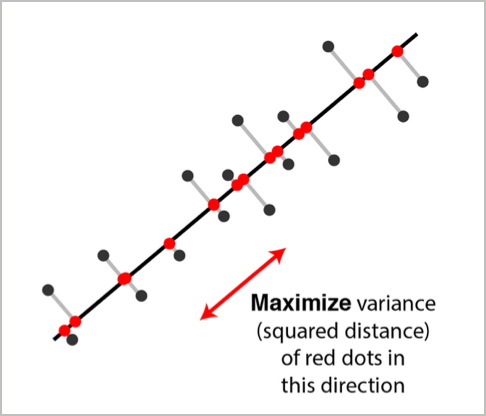
\includegraphics[width=0.3\textwidth]{variance-max}
\end{figure}
\begin{definition}[Sample Variance]
  The sample variance of the projected data is given by:
  \[\frac{1}{n}\sum_{i=1}^{n} {\left( \mathbf{u}^{[j]}\cdot\mathbf{x}^{(i)}-\mathbf{u}^{[j]}\cdot\bar{\mathbf{x}} \right)}^{2}=\mathbf{u}^{[j]T}\mathbf{Su}^{[j]}\] 
  The sample covariance matrix $\mathbf{S}$ is defned by:
\[\mathbf{S}=\frac{1}{n}\sum_{i=1}^{n} \left( \mathbf{x}^{(i)}-\bar{\mathbf{x}} \right) {\left( \mathbf{x}^{(i)}-\bar{\mathbf{x}} \right)}^{T}=\frac{1}{n}\mathbf{X}^{T}\mathbf{X}\] 
\end{definition}
where the centred design matrix $\mathbf{X}$ is defined:
\[\mathbf{X}=\begin{bmatrix} {\left( \mathbf{x}^{(1)}-\bar{\mathbf{x}}
\right)}^{T}\\ {\left( \mathbf{x}^{(2)}-\bar{\mathbf{x}}
\right)}^{T}\\\vdots\\{\left( \mathbf{x}^{(n)}-\bar{\mathbf{x}}
\right)}^{T}\end{bmatrix}.\] 
\begin{remark}
  PCA can also be viewed as a search for the $d$-dimensional subspace minmising
  the reconstruction error:
  \[\sum_{i=1}^{n} \left\lVert \left( \mathbf{x}^{(i)}-\bar{\mathbf{x}} \right) -\sum_{j=1}^{d} \left( \mathbf{u}^{[j]}\cdot\left( \mathbf{x}^{(i)}-\bar{\mathbf{x}} \right)  \right) \mathbf{u}^{[j]} \right\rVert_2^{2}.\]
  \begin{figure}[h!]
    \centering
    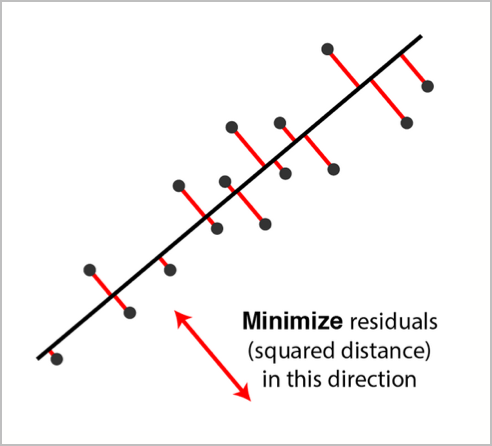
\includegraphics[width=0.3\textwidth]{residual-min}
  \end{figure}
\end{remark}

\subsubsection{Optimisation}
Re-writing our optimisation problem, we have:
\[\argmax_{{\left\{ \mathbf{u}^{[j]} \right\}}_{j=1}^{d}}L\quad\text{where:}\quad L=\sum_{j=1}^{d} \mathbf{u}^{[j]T}\mathbf{Su}^{[j]}.\]
for some orthonormal ${\left\{ \mathbf{u}^{[i]} \right\}}^{d}_{i=1}$.\\
In this algorithm, we attempt to learn each dimension greedily.
We first search for the direction of highest variance, and write the objective
as follows:
\[\mathcal{L}(\mathbf{u}^{[1]},\lambda^{[1]})=\mathbf{u}^{[1]T}\mathbf{Su}^{[1]}-\lambda^{[1]}\left( \mathbf{u}^{[1]}\cdot\mathbf{u}^{[1]}-1 \right)\] 
for some lagrange multiplier $\lambda^{[1]}$ associated with the orthogonality
constraint. Seeking stationarity w.r.t. $\mathbf{u}^{[1]}$, we have:
\begin{align*}
  2\mathbf{Su}^{[1]}-2\lambda^{[1]}\mathbf{u}^{[1]}=&0\\
  \implies\mathbf{Su}^{[1]}=&\lambda^{[1]}\mathbf{u}^{[1]}
\end{align*}
Hence $\mathbf{u}^{[1]}$ is an eigenvector of $\mathbf{S}$ associated with the
eigenvalue $\lambda^{[1]}$.  To find the variance of the projected data, we
have:
\[\mathbf{u}^{[1]T}\mathbf{Su}^{[1]}=\lambda^{[1]}\] 
To maximise this variance, we select the eigenvector associated with the
largest eigenvalue. We have found the first basis vector of greatest variance.
Now we seek to the second basis vector $\mathbf{u}^{[2]}$ to further increase
the projected variance, such that $\mathbf{u}^{[2]}\cdot \mathbf{u}^{[2]}=1$
and $\mathbf{u}^{[1]}\cdot \mathbf{u}^{[2]}=0$. We write the objective as
follows:
\[\mathcal{L}(\mathbf{u}^{[2]},\lambda^{[2]},\lambda^{[1][2]|})=\mathbf{u}^{[2]T}\mathbf{Su}^{[2]}-\lambda^{[2]}\left( \mathbf{u}^{[2]}\cdot\mathbf{u}^{[2]}-1 \right)-\lambda^{[1][2]}\left( \mathbf{u}^{[2]}\cdot\mathbf{u}^{[1]} -0\right) \] 
for some lagrange multipliers $\lambda^{[2]}, \lambda^{[1][2]}$. Seeking
stationarity w.r.t. $\mathbf{u}^{[2]}$, we have:
\[2\mathbf{Su}^{[2]}-2\lambda^{[2]}\mathbf{u}^{[2]}-\lambda^{[1][2]}\mathbf{u}^{[1]}=0.\] 
Left multiplying with $\mathbf{u}^{[1]T}$, $\lambda^{[1][2]}=0$.
Hence:
\[\mathbf{Su}^{[2]}=\lambda^{[2]}\mathbf{u}^{[2]}.\] 
Similarly, we want to maximise the variance so we select the eigenvector
associated with the largest remaining eigenvalue. The solution proceeds in a
similar step-wise fashion to give:
\[{\left\{ \mathbf{u}^{[j]*}=\mathbf{q}_j \right\}}_{j=1}^{d}\]
implying a total projected variance of:
\[L^{*}=\sum_{j=1}^{d} \mathbf{q}_j^{T}\mathbf{Sq}_j=\sum_{j=1}^{d} \lambda_j.\] 
This solution assumes orthogonality of basis vectors, normality of different
basis vectors and the orientation of the first basis vector. Other choices are
also possible yielding similar solutions. While the original problem is
non-convex, it is possible to show that the greedy local optima gives rise to
\textbf{globally optimal points}.\\
PCA allows estimation of the input space as the space spanned by the first $d$
eigenvectors with the largest eigenvalues of the sample covariance matrix.
\begin{definition}[Ambient and Intrinsic Dimensionalities]
  The dimensionality of the input space is known as the ambient dimensionality
  of the data, and the dimensionality of the subspace upon which the data is
  assumed to lie is known as the intrinsic dimensionality of the data.
\end{definition}
\subsubsection{Pattern Stabilility}
To be sure that the training sample has discerned a reliable subspace
(intuitively, how extensible the subspace is to other data) we consider two
other approaches:
\begin{itemize}
  \item \textbf{Generative Modelling}: Seeking a Gaussian latent variable model to be
    learned using MLE or Bayesian treatment
  \item \textbf{PAC Approach}: Bounding generalisation error resulting from
    projection $E_\mathcal{D}\left[ \mathbf{x}-\sum_{j=1}^{d} \left(
    \mathbf{u}^{[j]}\cdot\mathbf{x} \right) \mathbf{u}^{[j]} \right]$ with high
    probability. Bound consists terms in sample residual eigenspectrum and
    complexity of data space. With a subspace capturing a high proportion of
    the variance with a small relative dimensionality, we have low
    generalisation error.
\end{itemize}

\subsection{Probabilistic PCA}
In Probabilistic PCA, we seek a Gaussian latent variable model and learn its parameters
as a probabilistic generalisation of PCA.\@
\subsubsection{PPCA Model}
We assume that each point has an unknown latent variable $\mathbf{z}\in
\mathbb{R}^{d}$ associated with it corresponding to its position in the
principal component subspace. We assume this variable is a outcome of a Gaussian random variable
$\mathcal{Z}$:
\[\mathbf{z}\sim\mathcal{N}\left( \mathbf{0},\mathbf{I}_d \right).\] 
Additionally, each $\mathbf{x}$ is a outcome of a Gaussian random variable $\mathcal{X}$:
\[\mathbf{x|z}\sim\mathcal{N}\left( \mathbf{Wz+\mu},\sigma^{2}\mathbf{I}_m \right).\]
where $\mathbf{W}\in \mathbb{R}^{m\times d}$ defining the directions of the
principal subspace, $\mu\in \mathbb{R}^{m},\sigma\in \mathbb{R}^{+}$.\\

Intuitively, we can understand the model as follows:
\begin{itemize}
  \item We draw an outcome for the latent variable $\mathbf{z}$.
  \item The observed variable is sample conditional on the latent variable $\mathbf{x}|\mathbf{z}$.
  \item We observe residual noise $\varepsilon$ such that:
    \[\mathbf{x}=\mathbf{Wz+\mu+\varepsilon}.\] 
    \[\mathbf{z}\sim\mathcal{N}\left( \mathbf{0},\mathbf{I}_d \right).\] 
    \[\mathbf{\varepsilon}\sim\mathcal{N}\left( \mathbf{0},\sigma^{2}\mathbf{I}_m \right).\] 
    \begin{remark}
      Given a marginal distribution for $\mathbf{\tilde{x}}$ and a conditional
      Gaussian distribution for $\mathbf{\tilde{y}}$ given
      $\mathbf{\tilde{x}}$:
      \[\mathbf{\tilde{x}}\sim\mathcal{N}(\mathbf{\mu},\mathbf{\Lambda}^{-1})\] 
      \[\mathbf{\tilde{y}|\tilde{x}}\sim\mathcal{N}(\mathbf{A\tilde{x}+b},\mathbf{L}^{-1})\] 
      for some $\mathbf{\tilde{x}}\in \mathbb{R}^{n},\mathbf{\tilde{y}}\in \mathbb{R}^{m},\mathbf{\mu}\in \mathbb{R}^{n},\mathbf{\Lambda}\in \mathbb{R}^{n\times n},\mathbf{A}\in \mathbb{R}^{m\times n},\mathbf{b}\in \mathbb{R}^{m},\mathbf{L}\in \mathbb{R}\in ^{m\times m}$. Then:
    \[\mathbf{\tilde{y}}\sim\mathcal{N}\left( \mathbf{A\mu+b,L}^{-1}+\mathbf{A\Lambda}^{-1}\mathbf{A^{T}} \right).\] 
      \[\mathbf{\tilde{x}|\tilde{y}}\sim\mathcal{N}(\mathbf{\Sigma} \left[ \mathbf{A}^{T}\mathbf{L(\tilde{y}-b)+\Lambda\mu} \right],\mathbf{\Sigma})\] 
      where $\Sigma={(\mathbf{\Lambda}+\mathbf{A}^{T}\mathbf{LA})}^{-1}$
    \end{remark}
    Given this, we have:
    \[\mathbf{x}\sim\mathcal{N}\left( \mathbf{\mu},\mathbf{WW}^{T}+\sigma^{2}\mathbf{I}_m \right).\] 
\end{itemize}
Since the covariance matrix of the distribution of $\mathbf{x}$ is symmetric,
we can interpret $p_\mathcal{X}(\mathbf{x})$ as a density determined by
$\sigma^{2}$ of taking an isotropic Gaussian `spray can' across the principal
subspace. We have a `pancake' shaped distribution.
\subsubsection{Rotational Invariance}
Suppose $\mathbf{R}$ an orthogonal (rotation) matrix (hence $\mathbf{R}^{T}\mathbf{R}=\mathbf{I}$).
Applying it to the latent space coordinate matrix $\mathbf{W}$:
\begin{align*}
  \mathbf{\tilde{W}}=&\mathbf{WR}\\
  \implies\mathbf{\tilde{W}\tilde{W}}^{T}=&\mathbf{WRR}^{T}\mathbf{W}^{T}\\
  =&\mathbf{WW}^{T}
\end{align*}
The distribution of $\mathbf{x}$ can be characterised by any
$\mathbf{\tilde{W}}$. THis is the analogue of the non-uniqueness in PCA.\@
\subsubsection{Optimisation}
We find the log-likelihood function to optimise as follows:
\begin{align*}
  \mathcal{L}=&\sum_{i=1}^{n} \ln p_\mathcal{X}\left( \mathbf{x}^{(i)};\mathbf{W,\mu},\sigma^{2} \right) \\
  =&-\frac{nm}{2}\ln\left( 2\pi \right) -\frac{n}{2}\ln\left| \mathbf{C} \right| -\frac{1}{2}\sum_{i=1}^{n} {\left( \mathbf{x}^{(i)}-\mathbf{\mu} \right)}^{T}\mathbf{C}^{-1}\left( \mathbf{x}^{(i)}-\mathbf{\mu} \right) 
\end{align*}
It can be demonstrated that the following closed form solutions flow from the optimisation of this
function (Tipping \& Bishop, 1999):
\[\mathbf{\mu}_{MLE}=\mathbf{\bar{x}}.\]
\[\sigma_{MLE}=\frac{1}{m-d}\sum_{i=d+1}^{m} \lambda_i.\] 
\[\mathbf{W}_{MLE}=\mathbf{Q}{\left( \mathbf{\Lambda}-\sigma^{2}\mathbf{I} \right)}^{\frac{1}{2}\mathbf{R}}.\] 
where $\mathbf{Q}\in \mathbb{R}^{m\times d}$ whose columns are given by the
leading $d$ eigenvectors of the covariance matrix $\mathbf{S}$,
$\Lambda=\diag(\lambda_1,\lambda_2,\ldots,\lambda_d)$ contains the $d$
eigenvalues associated with these eigenvectors, and $\mathbf{R}$ is an
arbitrary orthogonal matrix. We can set $\mathbf{R=I}$ without loss of
generality, when $\mathbf{W}$ are the principal component eigenvectors scaled
by the square root of the variance parameters ${(\lambda_i-\sigma^{2})}^{\frac{1}{2}}$.
Hence, the variance of $p_\mathcal{X}(\mathbf{x})$ in the $\mathbf{q}_i$
direction is $\lambda_i$.


\section{Neural Networks}
\begin{definition}[Artificial Neuron]
  In neural networks, an artificial neuron is a mapping between some inputs
  $\mathbf{x}\in \mathbb{R}^{m}\mapsto\mathbb{R}$. It is defined by a weight
  vector $\mathbf{w}$ and a bias term $b$, and the sum is passed through an
  activation function:
  \[f(\mathbf{x})=\hat{\phi}\left( \mathbf{w\cdot x} +\mathbf{b}\right).\] 
\end{definition}
Often we take the logistic sigmoid $\hat{\phi}(z)=\frac{1}{1+e^{-z}}$, or the
heaviside function.  An Artificial Neural Network is a combination of many of
these units, how they are connected may be complex and is characterised by the
NN's architecture.
\begin{figure}[h!]
  \centering
  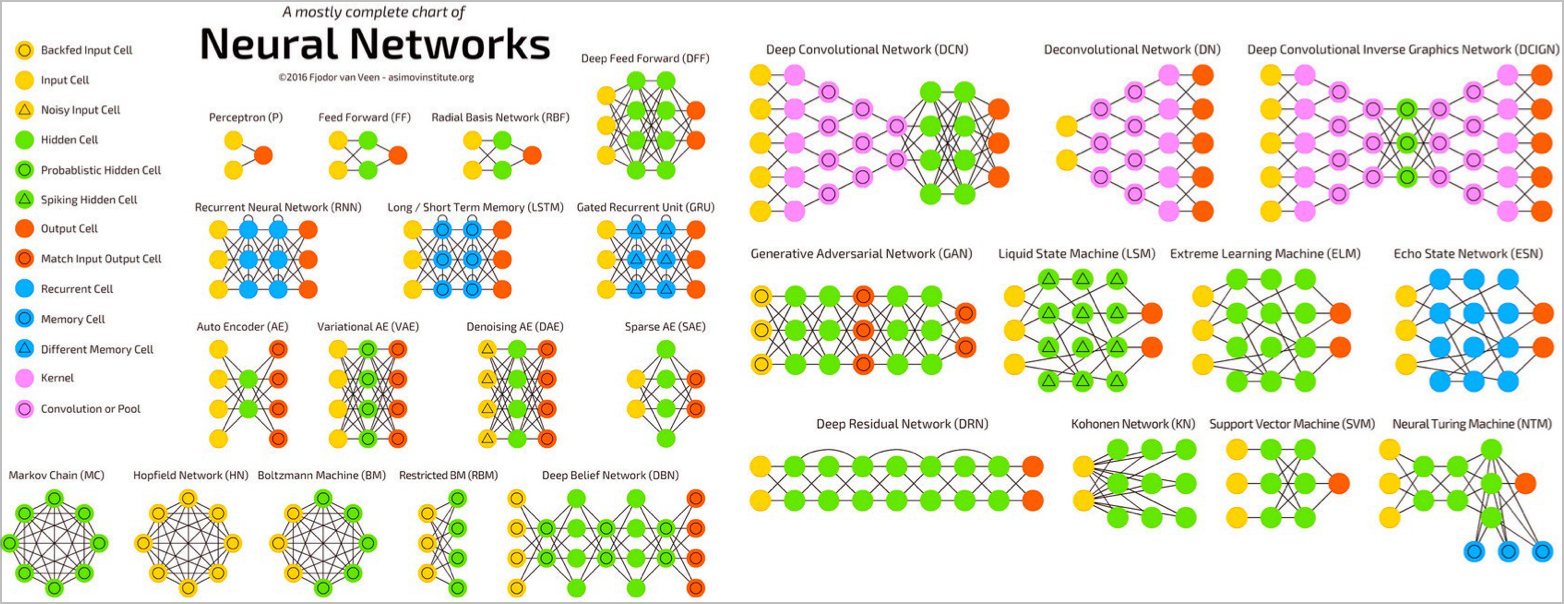
\includegraphics[width=0.8\textwidth]{neural-networks}
\end{figure}

We have two broad categories:
\begin{itemize}
  \item \textbf{Feed Forward Neural Networks}: where units are arranged into a graph without any
    cycles. This exploits the local structure of data, such as in a CNN.\@
  \item \textbf{Recurrent Neural Networks}: where the graph can have cycles
    such that outputs of a unit can loop back to become one of its inputs. This
    may be well used to perceive time series structures.
\end{itemize}

\subsection{Multilayer Perceptron}
A particular form of FFN where each layer contains some identical sigmoid
units, the Multilayer Perceptron (MLP) is fully connected (every unit in one
layer is connected to every layer in the next).
\begin{figure}[h!]
  \centering
  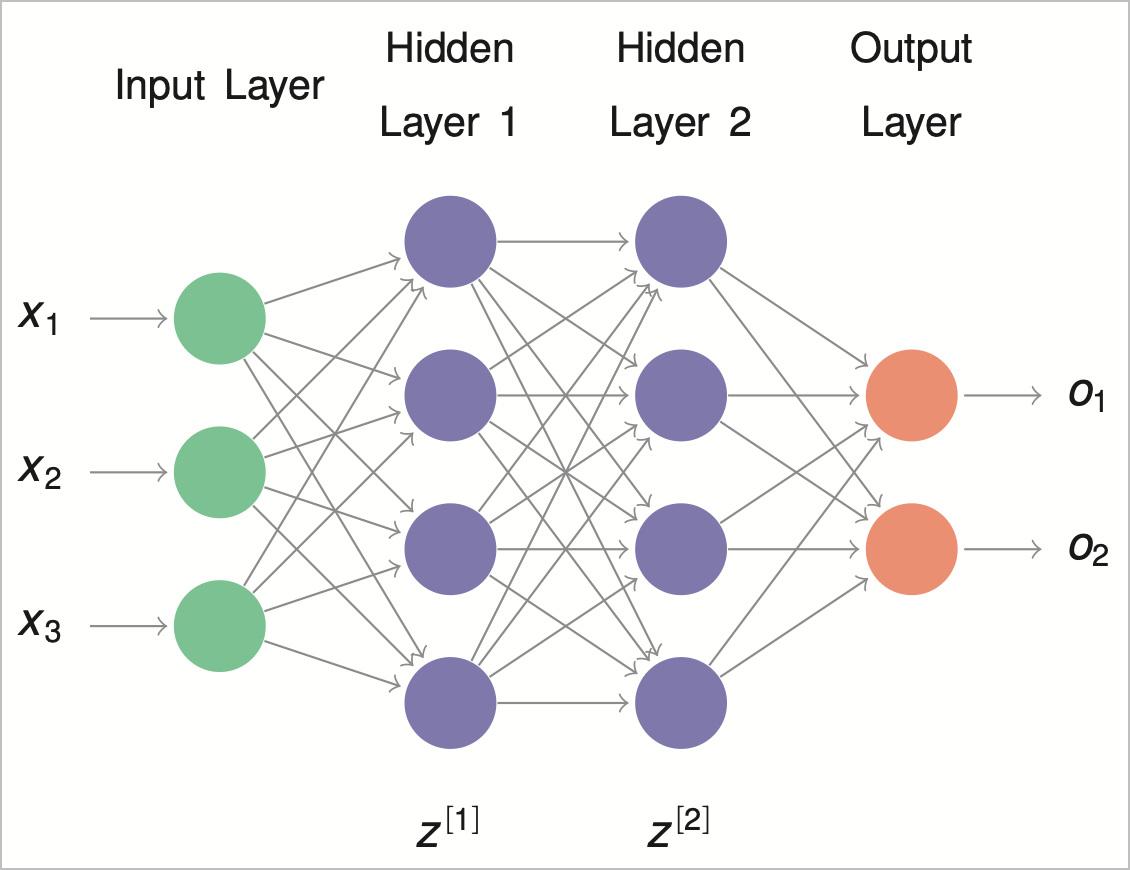
\includegraphics[width=0.6\textwidth]{mlp}
\end{figure}
We call the first layer the input layer, the last layer the output layer, and
those in between the hidden layers. The number of layers is the depth of the
MLP and the number of units in a layer is known as the width of the MLP.\@
We have in general:
\[z_i^{[h]}=\hat{\phi}\left( \sum_{j} w_{ij}^{[h]}z_j^{h-1}+b_i^{[h]} \right).\] 
\subsubsection{Feature Learning}
A NN is nonlinear mapping between a set of input variables $x$ to a set of
output variables $\left\{ o_i \right\}$ with functional forms controlled by
weights $\mathbf{w}$ to learn. Number of weights and basis functions are cosen
via our architecture, but they are adaptive through the weights. Features can
be learned implicitly with deeper layers learning more complex features.\\
Due to the non-linearity of activation functions, even a shallow MLP with just
one hidden layer can learn any non-linear function of the input. We call
MLP a \textbf{universal function approximator}, even though it might not be
compact.
\subsubsection{Evaluation}
For a $H$ hidden layer network, we have three canonical cases:
\begin{itemize}
  \item \textbf{Regression}: We have one output to be a linear function of
    units in the last layer 
    \[o^{(i)}=\sum_{j} w_j^{[H+1]}z_j^{[H](i)}+b^{[H+1]}\]
    and the evaluation function to be the squared loss
    \[L=\frac{1}{2}\sum_{i=1}^{n} {(o^{(i)-y^{(i)}})}^{2}\]
  \item \textbf{Binary Classification}: We have one output to be a logistic sigmoid
    function of units in the last layer
    \[o^{(i)}=\frac{1}{1+e^{-(\sum_{j} w_j^{[H+1]}z_j^{[H](i)}+b^{[H+1]})}}\]
    and the evaluation function to be the cross entropy
    \[L=-\sum_{i=1}^{n} y^{(i)}\ln(o^{(i)})+(1-y^{(i)})\ln(1-o^{(i)})\] 
  \item \textbf{Multi-Classification}: We have $K$ `initial' outputs from the
    last layer
    \[\tilde{o}_k^{(i)}=\sum_{j} w_j^{[H+1]}z_j^{[H](i)}+b^{[H+1]}\]
    of which we put through a softmax function to generate the final
    output units:
    \[o^{(i)}_k=\frac{\exp(\tilde{o}_k^{(i)})}{\sum_{j=1}^{K} \exp(\tilde{o}_j^{(i)})}\] 
    and the evaluation function to be the cross entropy
    \[L=-\sum_{i=1}^{n} \sum_{k=1}^{K} y_k^{(i)}\ln(\tilde{o}_k^{(i)})\] 
\end{itemize}
We evaluate $o^{(i)}$ for each of the training examples, as a forward pass
through the network from th e first hidden layer, second hidden layer and so
on. This process is known as the \textbf{forward propagation} of information
through the network.
\subsubsection{Optimisation}
For the output units we have $\delta_i^{[H+1]}=o-y$.
\[\delta_i^{[h]}=\hat{\phi}'\left( a_i^{[h]} \right) \sum_{k} w_{ki}^{[h+1]}\delta_k^{[h+1]}.\]

\end{document}
